\documentclass{article}

% if you need to pass options to natbib, use, e.g.:
%     \PassOptionsToPackage{numbers, compress}{natbib}
% before loading neurips_2021

% ready for submission
\usepackage{neurips_2021}

% to compile a preprint version, e.g., for submission to arXiv, add add the
% [preprint] option:
%     \usepackage[preprint]{neurips_2021}

% to compile a camera-ready version, add the [final] option, e.g.:
%     \usepackage[final]{neurips_2021}

% to avoid loading the natbib package, add option nonatbib:
%    \usepackage[nonatbib]{neurips_2021}

\usepackage[utf8]{inputenc} % allow utf-8 input
\usepackage[T1]{fontenc}    % use 8-bit T1 fonts
\usepackage{url}            % simple URL typesetting
\usepackage{booktabs}       % professional-quality tables
\usepackage{amsfonts}       % blackboard math symbols
\usepackage{nicefrac}       % compact symbols for 1/2, etc.
\usepackage{microtype}      % microtypography
%\usepackage{xcolor}         % colors
\usepackage[table]{xcolor}
%%%%% NEW MATH DEFINITIONS %%%%%
\usepackage{amsthm}
\usepackage{amsmath,amsfonts,bm}
\makeatletter
\newtheorem*{rep@theorem}{\rep@title}
\newcommand{\newreptheorem}[2]{%
\newenvironment{rep#1}[1]{%
 \def\rep@title{#2 \ref{##1}}%
 \begin{rep@theorem}}%
 {\end{rep@theorem}}}
\makeatother


\newtheorem{definition}{Definition}[section]
\newtheorem{theorem}{Theorem}
\newreptheorem{theorem}{Theorem}
\newtheorem{lemma}{Lemma}

\newcommand{\theHalgorithm}{\arabic{algorithm}}
\newenvironment{proofsketch}{%
  \renewcommand{\proofname}{Proof Sketch}\proof}{\endproof}
  
% Mark sections of captions for referring to divisions of figures
\newcommand{\RNum}[1]{\uppercase\expandafter{\romannumeral #1\relax}}
\newcommand{\mb}[1]{\mathbf{#1}}
\newcommand{\mbb}[1]{\mathbb{#1}}
\newcommand{\mc}[1]{\mathcal{#1}}
\newcommand{\tildex}{\tilde{\mb{x}}}
\newcommand{\figleft}{{\em (Left)}}
\newcommand{\figcenter}{{\em (Center)}}
\newcommand{\figright}{{\em (Right)}}
\newcommand{\figtop}{{\em (Top)}}
\newcommand{\figbottom}{{\em (Bottom)}}
\newcommand{\captiona}{{\em (a)}}
\newcommand{\captionb}{{\em (b)}}
\newcommand{\captionc}{{\em (c)}}
\newcommand{\captiond}{{\em (d)}}
\newcommand{\G}{\mathcal{G}}
\newcommand{\N}{\mathcal{N}}
\newcommand{\V}{\mathcal{V}}
\newcommand{\E}{\mathcal{E}}
\newcommand{\T}{\mathcal{T}}
\newcommand{\A}{\mathcal{A}}
\newcommand{\R}{\mathcal{R}}
\newcommand{\bx}{\mathbf{x}}
\newcommand{\by}{\mathbf{y}}
% Highlight a newly defined term
\newcommand{\newterm}[1]{{\bf #1}}
\usepackage{mathtools}
\DeclarePairedDelimiter{\ceil}{\lceil}{\rceil}
% Other
\def\defeq{\dot=}
\newcommand\norm[1]{\left\lVert#1\right\rVert} % Norm
\newcommand{\red}{\textcolor{red}}
\DeclareMathOperator*{\argmin}{\arg\!\min}
\DeclareMathOperator*{\argmax}{\arg\!\max}
\newcommand{\xhdr}[1]{{\noindent\bfseries #1}.}
\newcommand{\cut}[1]{}
\newcommand{\CITE}{\textcolor{red}{CITE}}
\newcommand{\will}[1]{\textcolor{cyan}{WILL: #1}}
\newcommand{\joey}[1]{\textcolor{RubineRed}{Joey: #1}}
\newcommand{\andjela}[1]{\textcolor{Green}{Andjela: #1}}
\newcommand{\hugo}[1]{\textcolor{orange}{Hugo: #1}}
\newcommand{\gauthier}[1]{\textcolor{purple}{Gauthier: #1}}
\newcommand{\removelatexerror}{\let\@latex@error\@gobble}

\newcommand{\GNN}{\textsc{GNN}}

% Figure reference, lower-case.
\def\figref#1{figure~\ref{#1}}
% Figure reference, capital. For start of sentence
\def\Figref#1{Figure~\ref{#1}}
\def\twofigref#1#2{figures \ref{#1} and \ref{#2}}
\def\quadfigref#1#2#3#4{figures \ref{#1}, \ref{#2}, \ref{#3} and \ref{#4}}
% Section reference, lower-case.
\def\secref#1{section~\ref{#1}}
% Section reference, capital.
\def\Secref#1{Section~\ref{#1}}
% Reference to two sections.
\def\twosecrefs#1#2{sections \ref{#1} and \ref{#2}}
% Reference to three sections.
\def\secrefs#1#2#3{sections \ref{#1}, \ref{#2} and \ref{#3}}
% Reference to an equation, lower-case.
\def\eqref#1{Eq.~\ref{#1}}
% Reference to an equation, upper case
\def\Eqref#1{Eq.~\ref{#1}}
% A raw reference to an equation---avoid using if possible
\def\plaineqref#1{\ref{#1}}
% Reference to a chapter, lower-case.
\def\chapref#1{chapter~\ref{#1}}
% Reference to an equation, upper case.
\def\Chapref#1{Chapter~\ref{#1}}
% Reference to a range of chapters
\def\rangechapref#1#2{chapters\ref{#1}--\ref{#2}}
% Reference to an algorithm, lower-case.
\def\algref#1{algorithm~\ref{#1}}
% Reference to an algorithm, upper case.
\def\Algref#1{Algorithm~\ref{#1}}
\def\twoalgref#1#2{algorithms \ref{#1} and \ref{#2}}
\def\Twoalgref#1#2{Algorithms \ref{#1} and \ref{#2}}
% Reference to a part, lower case
\def\partref#1{part~\ref{#1}}
% Reference to a part, upper case
\def\Partref#1{Part~\ref{#1}}
\def\twopartref#1#2{parts \ref{#1} and \ref{#2}}

\def\ceil#1{\lceil #1 \rceil}
\def\floor#1{\lfloor #1 \rfloor}
\def\1{\bm{1}}
\newcommand{\train}{\mathcal{D}}
\newcommand{\valid}{\mathcal{D_{\mathrm{valid}}}}
\newcommand{\test}{\mathcal{D_{\mathrm{test}}}}

\def\eps{{\epsilon}}


% Random variables
\def\reta{{\textnormal{$\eta$}}}
\def\ra{{\textnormal{a}}}
\def\rb{{\textnormal{b}}}
\def\rc{{\textnormal{c}}}
\def\rd{{\textnormal{d}}}
\def\re{{\textnormal{e}}}
\def\rf{{\textnormal{f}}}
\def\rg{{\textnormal{g}}}
\def\rh{{\textnormal{h}}}
\def\ri{{\textnormal{i}}}
\def\rj{{\textnormal{j}}}
\def\rk{{\textnormal{k}}}
\def\rl{{\textnormal{l}}}
% rm is already a command, just don't name any random variables m
\def\rn{{\textnormal{n}}}
\def\ro{{\textnormal{o}}}
\def\rp{{\textnormal{p}}}
\def\rq{{\textnormal{q}}}
\def\rr{{\textnormal{r}}}
\def\rs{{\textnormal{s}}}
\def\rt{{\textnormal{t}}}
\def\ru{{\textnormal{u}}}
\def\rv{{\textnormal{v}}}
\def\rw{{\textnormal{w}}}
\def\rx{{\textnormal{x}}}
\def\ry{{\textnormal{y}}}
\def\rz{{\textnormal{z}}}

% Random vectors
\def\rvepsilon{{\mathbf{\epsilon}}}
\def\rvtheta{{\mathbf{\theta}}}
\def\rva{{\mathbf{a}}}
\def\rvb{{\mathbf{b}}}
\def\rvc{{\mathbf{c}}}
\def\rvd{{\mathbf{d}}}
\def\rve{{\mathbf{e}}}
\def\rvf{{\mathbf{f}}}
\def\rvg{{\mathbf{g}}}
\def\rvh{{\mathbf{h}}}
\def\rvu{{\mathbf{i}}}
\def\rvj{{\mathbf{j}}}
\def\rvk{{\mathbf{k}}}
\def\rvl{{\mathbf{l}}}
\def\rvm{{\mathbf{m}}}
\def\rvn{{\mathbf{n}}}
\def\rvo{{\mathbf{o}}}
\def\rvp{{\mathbf{p}}}
\def\rvq{{\mathbf{q}}}
\def\rvr{{\mathbf{r}}}
\def\rvs{{\mathbf{s}}}
\def\rvt{{\mathbf{t}}}
\def\rvu{{\mathbf{u}}}
\def\rvv{{\mathbf{v}}}
\def\rvw{{\mathbf{w}}}
\def\rvx{{\mathbf{x}}}
\def\rvy{{\mathbf{y}}}
\def\rvz{{\mathbf{z}}}

% Elements of random vectors
\def\erva{{\textnormal{a}}}
\def\ervb{{\textnormal{b}}}
\def\ervc{{\textnormal{c}}}
\def\ervd{{\textnormal{d}}}
\def\erve{{\textnormal{e}}}
\def\ervf{{\textnormal{f}}}
\def\ervg{{\textnormal{g}}}
\def\ervh{{\textnormal{h}}}
\def\ervi{{\textnormal{i}}}
\def\ervj{{\textnormal{j}}}
\def\ervk{{\textnormal{k}}}
\def\ervl{{\textnormal{l}}}
\def\ervm{{\textnormal{m}}}
\def\ervn{{\textnormal{n}}}
\def\ervo{{\textnormal{o}}}
\def\ervp{{\textnormal{p}}}
\def\ervq{{\textnormal{q}}}
\def\ervr{{\textnormal{r}}}
\def\ervs{{\textnormal{s}}}
\def\ervt{{\textnormal{t}}}
\def\ervu{{\textnormal{u}}}
\def\ervv{{\textnormal{v}}}
\def\ervw{{\textnormal{w}}}
\def\ervx{{\textnormal{x}}}
\def\ervy{{\textnormal{y}}}
\def\ervz{{\textnormal{z}}}

% Random matrices
\def\rmA{{\mathbf{A}}}
\def\rmB{{\mathbf{B}}}
\def\rmC{{\mathbf{C}}}
\def\rmD{{\mathbf{D}}}
\def\rmE{{\mathbf{E}}}
\def\rmF{{\mathbf{F}}}
\def\rmG{{\mathbf{G}}}
\def\rmH{{\mathbf{H}}}
\def\rmI{{\mathbf{I}}}
\def\rmJ{{\mathbf{J}}}
\def\rmK{{\mathbf{K}}}
\def\rmL{{\mathbf{L}}}
\def\rmM{{\mathbf{M}}}
\def\rmN{{\mathbf{N}}}
\def\rmO{{\mathbf{O}}}
\def\rmP{{\mathbf{P}}}
\def\rmQ{{\mathbf{Q}}}
\def\rmR{{\mathbf{R}}}
\def\rmS{{\mathbf{S}}}
\def\rmT{{\mathbf{T}}}
\def\rmU{{\mathbf{U}}}
\def\rmV{{\mathbf{V}}}
\def\rmW{{\mathbf{W}}}
\def\rmX{{\mathbf{X}}}
\def\rmY{{\mathbf{Y}}}
\def\rmZ{{\mathbf{Z}}}

% Elements of random matrices
\def\ermA{{\textnormal{A}}}
\def\ermB{{\textnormal{B}}}
\def\ermC{{\textnormal{C}}}
\def\ermD{{\textnormal{D}}}
\def\ermE{{\textnormal{E}}}
\def\ermF{{\textnormal{F}}}
\def\ermG{{\textnormal{G}}}
\def\ermH{{\textnormal{H}}}
\def\ermI{{\textnormal{I}}}
\def\ermJ{{\textnormal{J}}}
\def\ermK{{\textnormal{K}}}
\def\ermL{{\textnormal{L}}}
\def\ermM{{\textnormal{M}}}
\def\ermN{{\textnormal{N}}}
\def\ermO{{\textnormal{O}}}
\def\ermP{{\textnormal{P}}}
\def\ermQ{{\textnormal{Q}}}
\def\ermR{{\textnormal{R}}}
\def\ermS{{\textnormal{S}}}
\def\ermT{{\textnormal{T}}}
\def\ermU{{\textnormal{U}}}
\def\ermV{{\textnormal{V}}}
\def\ermW{{\textnormal{W}}}
\def\ermX{{\textnormal{X}}}
\def\ermY{{\textnormal{Y}}}
\def\ermZ{{\textnormal{Z}}}

% Vectors
\def\vzero{{\bm{0}}}
\def\vone{{\bm{1}}}
\def\vmu{{\bm{\mu}}}
\def\vtheta{{\bm{\theta}}}
\def\va{{\bm{a}}}
\def\vb{{\bm{b}}}
\def\vc{{\bm{c}}}
\def\vd{{\bm{d}}}
\def\ve{{\bm{e}}}
\def\vf{{\bm{f}}}
\def\vg{{\bm{g}}}
\def\vh{{\bm{h}}}
\def\vi{{\bm{i}}}
\def\vj{{\bm{j}}}
\def\vk{{\bm{k}}}
\def\vl{{\bm{l}}}
\def\vm{{\bm{m}}}
\def\vn{{\bm{n}}}
\def\vo{{\bm{o}}}
\def\vp{{\bm{p}}}
\def\vq{{\bm{q}}}
\def\vr{{\bm{r}}}
\def\vs{{\bm{s}}}
\def\vt{{\bm{t}}}
\def\vu{{\bm{u}}}
\def\vv{{\bm{v}}}
\def\vw{{\bm{w}}}
\def\vx{{\bm{x}}}
\def\vy{{\bm{y}}}
\def\vz{{\bm{z}}}

% Elements of vectors
\def\evalpha{{\alpha}}
\def\evbeta{{\beta}}
\def\evepsilon{{\epsilon}}
\def\evlambda{{\lambda}}
\def\evomega{{\omega}}
\def\evmu{{\mu}}
\def\evpsi{{\psi}}
\def\evsigma{{\sigma}}
\def\evtheta{{\theta}}
\def\eva{{a}}
\def\evb{{b}}
\def\evc{{c}}
\def\evd{{d}}
\def\eve{{e}}
\def\evf{{f}}
\def\evg{{g}}
\def\evh{{h}}
\def\evi{{i}}
\def\evj{{j}}
\def\evk{{k}}
\def\evl{{l}}
\def\evm{{m}}
\def\evn{{n}}
\def\evo{{o}}
\def\evp{{p}}
\def\evq{{q}}
\def\evr{{r}}
\def\evs{{s}}
\def\evt{{t}}
\def\evu{{u}}
\def\evv{{v}}
\def\evw{{w}}
\def\evx{{x}}
\def\evy{{y}}
\def\evz{{z}}

% Matrix
\def\mA{{\bm{A}}}
\def\mB{{\bm{B}}}
\def\mC{{\bm{C}}}
\def\mD{{\bm{D}}}
\def\mE{{\bm{E}}}
\def\mF{{\bm{F}}}
\def\mG{{\bm{G}}}
\def\mH{{\bm{H}}}
\def\mI{{\bm{I}}}
\def\mJ{{\bm{J}}}
\def\mK{{\bm{K}}}
\def\mL{{\bm{L}}}
\def\mM{{\bm{M}}}
\def\mN{{\bm{N}}}
\def\mO{{\bm{O}}}
\def\mP{{\bm{P}}}
\def\mQ{{\bm{Q}}}
\def\mR{{\bm{R}}}
\def\mS{{\bm{S}}}
\def\mT{{\bm{T}}}
\def\mU{{\bm{U}}}
\def\mV{{\bm{V}}}
\def\mW{{\bm{W}}}
\def\mX{{\bm{X}}}
\def\mY{{\bm{Y}}}
\def\mZ{{\bm{Z}}}
\def\mBeta{{\bm{\beta}}}
\def\mPhi{{\bm{\Phi}}}
\def\mLambda{{\bm{\Lambda}}}
\def\mSigma{{\bm{\Sigma}}}

% Tensor
\DeclareMathAlphabet{\mathsfit}{\encodingdefault}{\sfdefault}{m}{sl}
\SetMathAlphabet{\mathsfit}{bold}{\encodingdefault}{\sfdefault}{bx}{n}
\newcommand{\tens}[1]{\bm{\mathsfit{#1}}}
\def\tA{{\tens{A}}}
\def\tB{{\tens{B}}}
\def\tC{{\tens{C}}}
\def\tD{{\tens{D}}}
\def\tE{{\tens{E}}}
\def\tF{{\tens{F}}}
\def\tG{{\tens{G}}}
\def\tH{{\tens{H}}}
\def\tI{{\tens{I}}}
\def\tJ{{\tens{J}}}
\def\tK{{\tens{K}}}
\def\tL{{\tens{L}}}
\def\tM{{\tens{M}}}
\def\tN{{\tens{N}}}
\def\tO{{\tens{O}}}
\def\tP{{\tens{P}}}
\def\tQ{{\tens{Q}}}
\def\tR{{\tens{R}}}
\def\tS{{\tens{S}}}
\def\tT{{\tens{T}}}
\def\tU{{\tens{U}}}
\def\tV{{\tens{V}}}
\def\tW{{\tens{W}}}
\def\tX{{\tens{X}}}
\def\tY{{\tens{Y}}}
\def\tZ{{\tens{Z}}}


% Graph
\def\gA{{\mathcal{A}}}
\def\gB{{\mathcal{B}}}
\def\gC{{\mathcal{C}}}
\def\gD{{\mathcal{D}}}
\def\gE{{\mathcal{E}}}
\def\gF{{\mathcal{F}}}
\def\gG{{\mathcal{G}}}
\def\gH{{\mathcal{H}}}
\def\gI{{\mathcal{I}}}
\def\gJ{{\mathcal{J}}}
\def\gK{{\mathcal{K}}}
\def\gL{{\mathcal{L}}}
\def\gM{{\mathcal{M}}}
\def\gN{{\mathcal{N}}}
\def\gO{{\mathcal{O}}}
\def\gP{{\mathcal{P}}}
\def\gQ{{\mathcal{Q}}}
\def\gR{{\mathcal{R}}}
\def\gS{{\mathcal{S}}}
\def\gT{{\mathcal{T}}}
\def\gU{{\mathcal{U}}}
\def\gV{{\mathcal{V}}}
\def\gW{{\mathcal{W}}}
\def\gX{{\mathcal{X}}}
\def\gY{{\mathcal{Y}}}
\def\gZ{{\mathcal{Z}}}

% Sets
\def\sA{{\mathbb{A}}}
\def\sB{{\mathbb{B}}}
\def\sC{{\mathbb{C}}}
\def\sD{{\mathbb{D}}}
% Don't use a set called E, because this would be the same as our symbol
% for expectation.
\def\sE{{\mathbb{E}}}
\def\sF{{\mathbb{F}}}
\def\sG{{\mathbb{G}}}
\def\sH{{\mathbb{H}}}
\def\sI{{\mathbb{I}}}
\def\sJ{{\mathbb{J}}}
\def\sK{{\mathbb{K}}}
\def\sL{{\mathbb{L}}}
\def\sM{{\mathbb{M}}}
\def\sN{{\mathbb{N}}}
\def\sO{{\mathbb{O}}}
\def\sP{{\mathbb{P}}}
\def\sQ{{\mathbb{Q}}}
\def\sR{{\mathbb{R}}}
\def\sS{{\mathbb{S}}}
\def\sT{{\mathbb{T}}}
\def\sU{{\mathbb{U}}}
\def\sV{{\mathbb{V}}}
\def\sW{{\mathbb{W}}}
\def\sX{{\mathbb{X}}}
\def\sY{{\mathbb{Y}}}
\def\sZ{{\mathbb{Z}}}

% Entries of a matrix
\def\emLambda{{\Lambda}}
\def\emA{{A}}
\def\emB{{B}}
\def\emC{{C}}
\def\emD{{D}}
\def\emE{{E}}
\def\emF{{F}}
\def\emG{{G}}
\def\emH{{H}}
\def\emI{{I}}
\def\emJ{{J}}
\def\emK{{K}}
\def\emL{{L}}
\def\emM{{M}}
\def\emN{{N}}
\def\emO{{O}}
\def\emP{{P}}
\def\emQ{{Q}}
\def\emR{{R}}
\def\emS{{S}}
\def\emT{{T}}
\def\emU{{U}}
\def\emV{{V}}
\def\emW{{W}}
\def\emX{{X}}
\def\emY{{Y}}
\def\emZ{{Z}}
\def\emSigma{{\Sigma}}

% entries of a tensor
% Same font as tensor, without \bm wrapper
\newcommand{\etens}[1]{\mathsfit{#1}}
\def\etLambda{{\etens{\Lambda}}}
\def\etA{{\etens{A}}}
\def\etB{{\etens{B}}}
\def\etC{{\etens{C}}}
\def\etD{{\etens{D}}}
\def\etE{{\etens{E}}}
\def\etF{{\etens{F}}}
\def\etG{{\etens{G}}}
\def\etH{{\etens{H}}}
\def\etI{{\etens{I}}}
\def\etJ{{\etens{J}}}
\def\etK{{\etens{K}}}
\def\etL{{\etens{L}}}
\def\etM{{\etens{M}}}
\def\etN{{\etens{N}}}
\def\etO{{\etens{O}}}
\def\etP{{\etens{P}}}
\def\etQ{{\etens{Q}}}
\def\etR{{\etens{R}}}
\def\etS{{\etens{S}}}
\def\etT{{\etens{T}}}
\def\etU{{\etens{U}}}
\def\etV{{\etens{V}}}
\def\etW{{\etens{W}}}
\def\etX{{\etens{X}}}
\def\etY{{\etens{Y}}}
\def\etZ{{\etens{Z}}}

% The true underlying data generating distribution
\newcommand{\pdata}{p_{\rm{data}}}
% The empirical distribution defined by the training set
\newcommand{\ptrain}{\hat{p}_{\rm{data}}}
\newcommand{\Ptrain}{\hat{P}_{\rm{data}}}
% The model distribution
\newcommand{\pmodel}{p_{\rm{model}}}
\newcommand{\Pmodel}{P_{\rm{model}}}
\newcommand{\ptildemodel}{\tilde{p}_{\rm{model}}}
% Stochastic autoencoder distributions
\newcommand{\pencode}{p_{\rm{encoder}}}
\newcommand{\pdecode}{p_{\rm{decoder}}}
\newcommand{\precons}{p_{\rm{reconstruct}}}

\newcommand{\laplace}{\mathrm{Laplace}} % Laplace distribution

%\newcommand{\E}{\mathbb{E}}
\newcommand{\Ls}{\mathcal{L}}
%\newcommand{\R}{\mathbb{R}}
\newcommand{\emp}{\tilde{p}}
\newcommand{\lr}{\alpha}
\newcommand{\reg}{\lambda}
\newcommand{\rect}{\mathrm{rectifier}}
\newcommand{\softmax}{\mathrm{softmax}}
\newcommand{\sigmoid}{\sigma}
\newcommand{\softplus}{\zeta}
\newcommand{\KL}{D_{\mathrm{KL}}}
\newcommand{\Var}{\mathrm{Var}}
\newcommand{\standarderror}{\mathrm{SE}}
\newcommand{\Cov}{\mathrm{Cov}}
% Wolfram Mathworld says $L^2$ is for function spaces and $\ell^2$ is for vectors
% But then they seem to use $L^2$ for vectors throughout the site, and so does
% wikipedia.
\newcommand{\normlzero}{L^0}
\newcommand{\normlone}{L^1}
\newcommand{\normltwo}{L^2}
\newcommand{\normlp}{L^p}
\newcommand{\normmax}{L^\infty}

\newcommand{\parents}{Pa} % See usage in notation.tex. Chosen to match Daphne's book.

%\DeclareMathOperator*{\argmax}{arg\,max}
%\DeclareMathOperator*{\argmin}{arg\,min}

\DeclareMathOperator{\sign}{sign}
\DeclareMathOperator{\Tr}{Tr}
\DeclareMathOperator{\sech}{sech}
\DeclareMathOperator{\csch}{csch}
\DeclareMathOperator{\arcsec}{arcsec}
\DeclareMathOperator{\arccot}{arccot}
\DeclareMathOperator{\arccsc}{arccsc}
\DeclareMathOperator{\arccosh}{arccosh}
\DeclareMathOperator{\arcsinh}{arcsinh}
\DeclareMathOperator{\arctanh}{arctanh}
\DeclareMathOperator{\arcsech}{arcsech}
\DeclareMathOperator{\arccsch}{arccsch}
\DeclareMathOperator{\arccoth}{arccoth} 
\let\ab\allowbreak

\usepackage[utf8]{inputenc}
%\usepackage{natbib}

\usepackage{multirow}
\usepackage{mathtools}
\usepackage{tikz}
\usetikzlibrary{fit,calc}
\usetikzlibrary{tikzmark}
% \usepackage{hyperref}
\usepackage{url}
\usepackage{graphicx}
\usepackage{amsmath}
\usepackage{enumitem}
\usepackage{mdframed}
%\usepackage[square,numbers]{natbib}
\usepackage{natbib}
\usepackage{bbm}
\usepackage[utf8]{inputenc}
\usepackage[english]{babel}
\usepackage{soul}
\usepackage{amsthm}
\usepackage{algorithm}
\usepackage[noend]{algorithmic}
% Attempt to make hyperref and algorithmic work together better:
\usepackage{color}
\usepackage{comment}
\usepackage{wrapfig}
\usepackage{caption}
\usepackage{subcaption}
\usepackage{footmisc}

\newcommand*{\tikzmk}[1]{\tikz[remember picture,overlay,] \node (#1) {};\ignorespaces}
\newcounter{ggiCounter}
\newcommand{\ggi}[1]{{\small \color{mydarkblue}
\refstepcounter{ggiCounter}\textsf{[ggi]$_{\arabic{ggiCounter}}$:{#1}}}}
%define a boxing command, argument = colour of box
\newcommand{\boxit}[1]{\tikz[remember picture,overlay]{\node[yshift=-12pt, xshift=-7pt, fill=#1,opacity=.25,fit={(A)($(B)+(-0.09\linewidth,.8)$)}] {};}\ignorespaces}

\newcommand{\boxittwo}[1]{\tikz[remember picture,overlay]{\node[yshift=-12pt, xshift=-7pt, fill=#1,opacity=.9,fit={(A)($(B)+(-0.09\linewidth,.8)$)}] {};}\ignorespaces}
%define some colours according to algorithm parts (or any other method you like)
\colorlet{pink}{red!40}
\colorlet{blue}{cyan!60}
\setstcolor{red}

\newcommand{\algoname}{\textsc{Virtual+}}
\newcommand{\setvalue}{$\mathbb{V}$}
\newcommand{\setvaluemath}{\mathbb{V}}
\definecolor{mydarkblue}{rgb}{0,0.08,0.45}

\definecolor{grannysmithapple}{rgb}{0.79, 0.92, 0.77}
\definecolor{darkgrannysmithapple}{rgb}{0.79, 0.99, 0.77}
\definecolor{g1}{HTML}{8FC771}
\definecolor{g2}{HTML}{B4D375}
\definecolor{g3}{HTML}{DADF79}
\definecolor{g4}{HTML}{FFEB7D}

\definecolor{salmon}{HTML}{FF8C94}

\definecolor{mydarkblue}{rgb}{0,0.08,0.45}
\usepackage[colorlinks=true,
    linkcolor=mydarkblue,
    citecolor=mydarkblue,
    filecolor=mydarkblue,
    urlcolor=mydarkblue]{hyperref}  
\usepackage{soul}
\setstcolor{pink}
\setul{}{1pt}
\newtheorem*{theo}{Online Threat Model}
\newenvironment{ftheo}
  {\begin{mdframed}\begin{theo}}
  {\end{theo}\end{mdframed}}



\title{Online Adversarial Attacks}

% The \author macro works with any number of authors. There are two commands
% used to separate the names and addresses of multiple authors: \And and \AND.
%
% Using \And between authors leaves it to LaTeX to determine where to break the
% lines. Using \AND forces a line break at that point. So, if LaTeX puts 3 of 4
% authors names on the first line, and the last on the second line, try using
% \AND instead of \And before the third author name.

\author{%
  David S.~Hippocampus\thanks{Use footnote for providing further information
    about author (webpage, alternative address)---\emph{not} for acknowledging
    funding agencies.} \\
  Department of Computer Science\\
  Cranberry-Lemon University\\
  Pittsburgh, PA 15213 \\
  \texttt{hippo@cs.cranberry-lemon.edu} \\
  % examples of more authors
  % \And
  % Coauthor \\
  % Affiliation \\
  % Address \\
  % \texttt{email} \\
  % \AND
  % Coauthor \\
  % Affiliation \\
  % Address \\
  % \texttt{email} \\
  % \And
  % Coauthor \\
  % Affiliation \\
  % Address \\
  % \texttt{email} \\
  % \And
  % Coauthor \\
  % Affiliation \\
  % Address \\
  % \texttt{email} \\
}

\begin{document}

\maketitle

\begin{abstract}
 Adversarial attacks expose important vulnerabilities of deep learning models, yet little attention has been paid to settings where data arrives as a stream. In this paper, we formalize the online adversarial attack problem, emphasizing two key elements found in real-world use-cases: attackers must operate under partial knowledge of the target model, and the decisions made by the attacker are irrevocable since they operate on a transient data stream. We first rigorously analyze a deterministic variant of the online threat model by drawing parallels to the well-studied $k$-secretary problem in theoretical computer science and propose \algoname, a simple yet practical online algorithm. Our main theoretical result show \algoname \ yields provably the best competitive ratio over all single-threshold algorithms for $k<5$---extending previous analysis of the $k$-secretary problem. We also introduce the \textit{stochastic $k$-secretary}---effectively reducing online blackbox transfer attacks to a $k$-secretary problem under noise---and prove theoretical bounds on the performance of \textit{any} online algorithms adapted to this setting. Finally, we complement our theoretical results by conducting experiments on both MNIST and CIFAR-10 with both vanilla and robust classifiers, revealing not only the necessity of online algorithms in achieving near-optimal performance but also the rich interplay of a given attack strategy towards online attack selection, enabling simple strategies like FGSM to outperform classically strong whitebox adversaries.
\end{abstract}


% Old Abstract
\cut{
 Adversarial attacks expose important vulnerabilities of deep learning models, yet little attention has been paid to settings where data arrives as a stream. In this paper, we formalize the online adversarial attack problem, emphasizing two key elements found in real-world use-cases: attackers must operate under partial knowledge of the target model, and the decisions made by the attacker are irrevocable since they operate on a transient data stream. We first rigorously analyze a deterministic variant of the online threat model by drawing parallels to the well-studied $k$-\textit{secretary problem} and propose \algoname, a simple yet practical online algorithm yielding a provably better competitive ratio for $k=2$ over the current best single threshold algorithm. We also introduce the \textit{stochastic $k$-secretary}---effectively reducing online blackbox transfer attacks to a $k$-secretary problem under noise---and prove theoretical bounds on the competitive ratios of \textit{any} online algorithms adapted to this setting. Finally, we complement our theoretical results by conducting a systematic suite of experiments on MNIST and CIFAR-10 with both vanilla and robust classifiers, revealing that, by leveraging online secretary algorithms, like \algoname, we can get an online attack success rate close to the one achieved by the optimal offline solution. 
}

\section{Introduction}


In adversarial attacks, an attacker seeks to maliciously disrupt the performance of deep learning systems by adding small but often imperceptible noise to otherwise clean data~\citep{szegedy2013intriguing,goodfellow2014explaining}. Critical to the study of adversarial attacks is specifying the threat model~\cite{akhtar2018threat}, which outlines the adversarial capabilities of an attacker and the level of information available in crafting attacks. Canonical examples include the \textit{whitebox} threat model~\cite{madry2017towards}, where the attacker has complete access, and the less permissive \textit{blackbox} threat model where an attacker only has partial information, like the ability to query the target model \citep{chen2017zoo,ilyas2017query,papernot2016transferability}. 

Previously studied threat models (e.g., whitebox and blackbox) implicitly assume a static setting that permits full access to instances in a target dataset at all times~\citep{tramer2017ensemble}. However, such an assumption is unrealistic in many real-world systems. Countless real-world applications involve streaming data that arrive in an online fashion (e.g., financial markets or real-time sensor networks). Understanding the feasibility of adversarial attacks in this {\em online} setting is an essential question. 

As a motivating example, consider the case where the adversary launches a man-in-the-middle attack depicted in Fig.~\ref{fig:man_in_the_middle}. Here, data is streamed between two endpoints---i.e., from sensors on an autonomous car to the actual control system. 
An adversary, in this example, would intercept the sensor data, potentially perturb it, and then send it to the controller. Unlike classical adversarial attacks, such a scenario presents two key challenges that are representative of all online settings. 

\begin{wrapfigure}{o}{0.4\textwidth}
  \vspace{-12pt}
  %\begin{center}
    %\includegraphics[width=0.48\textwidth]{birds}
    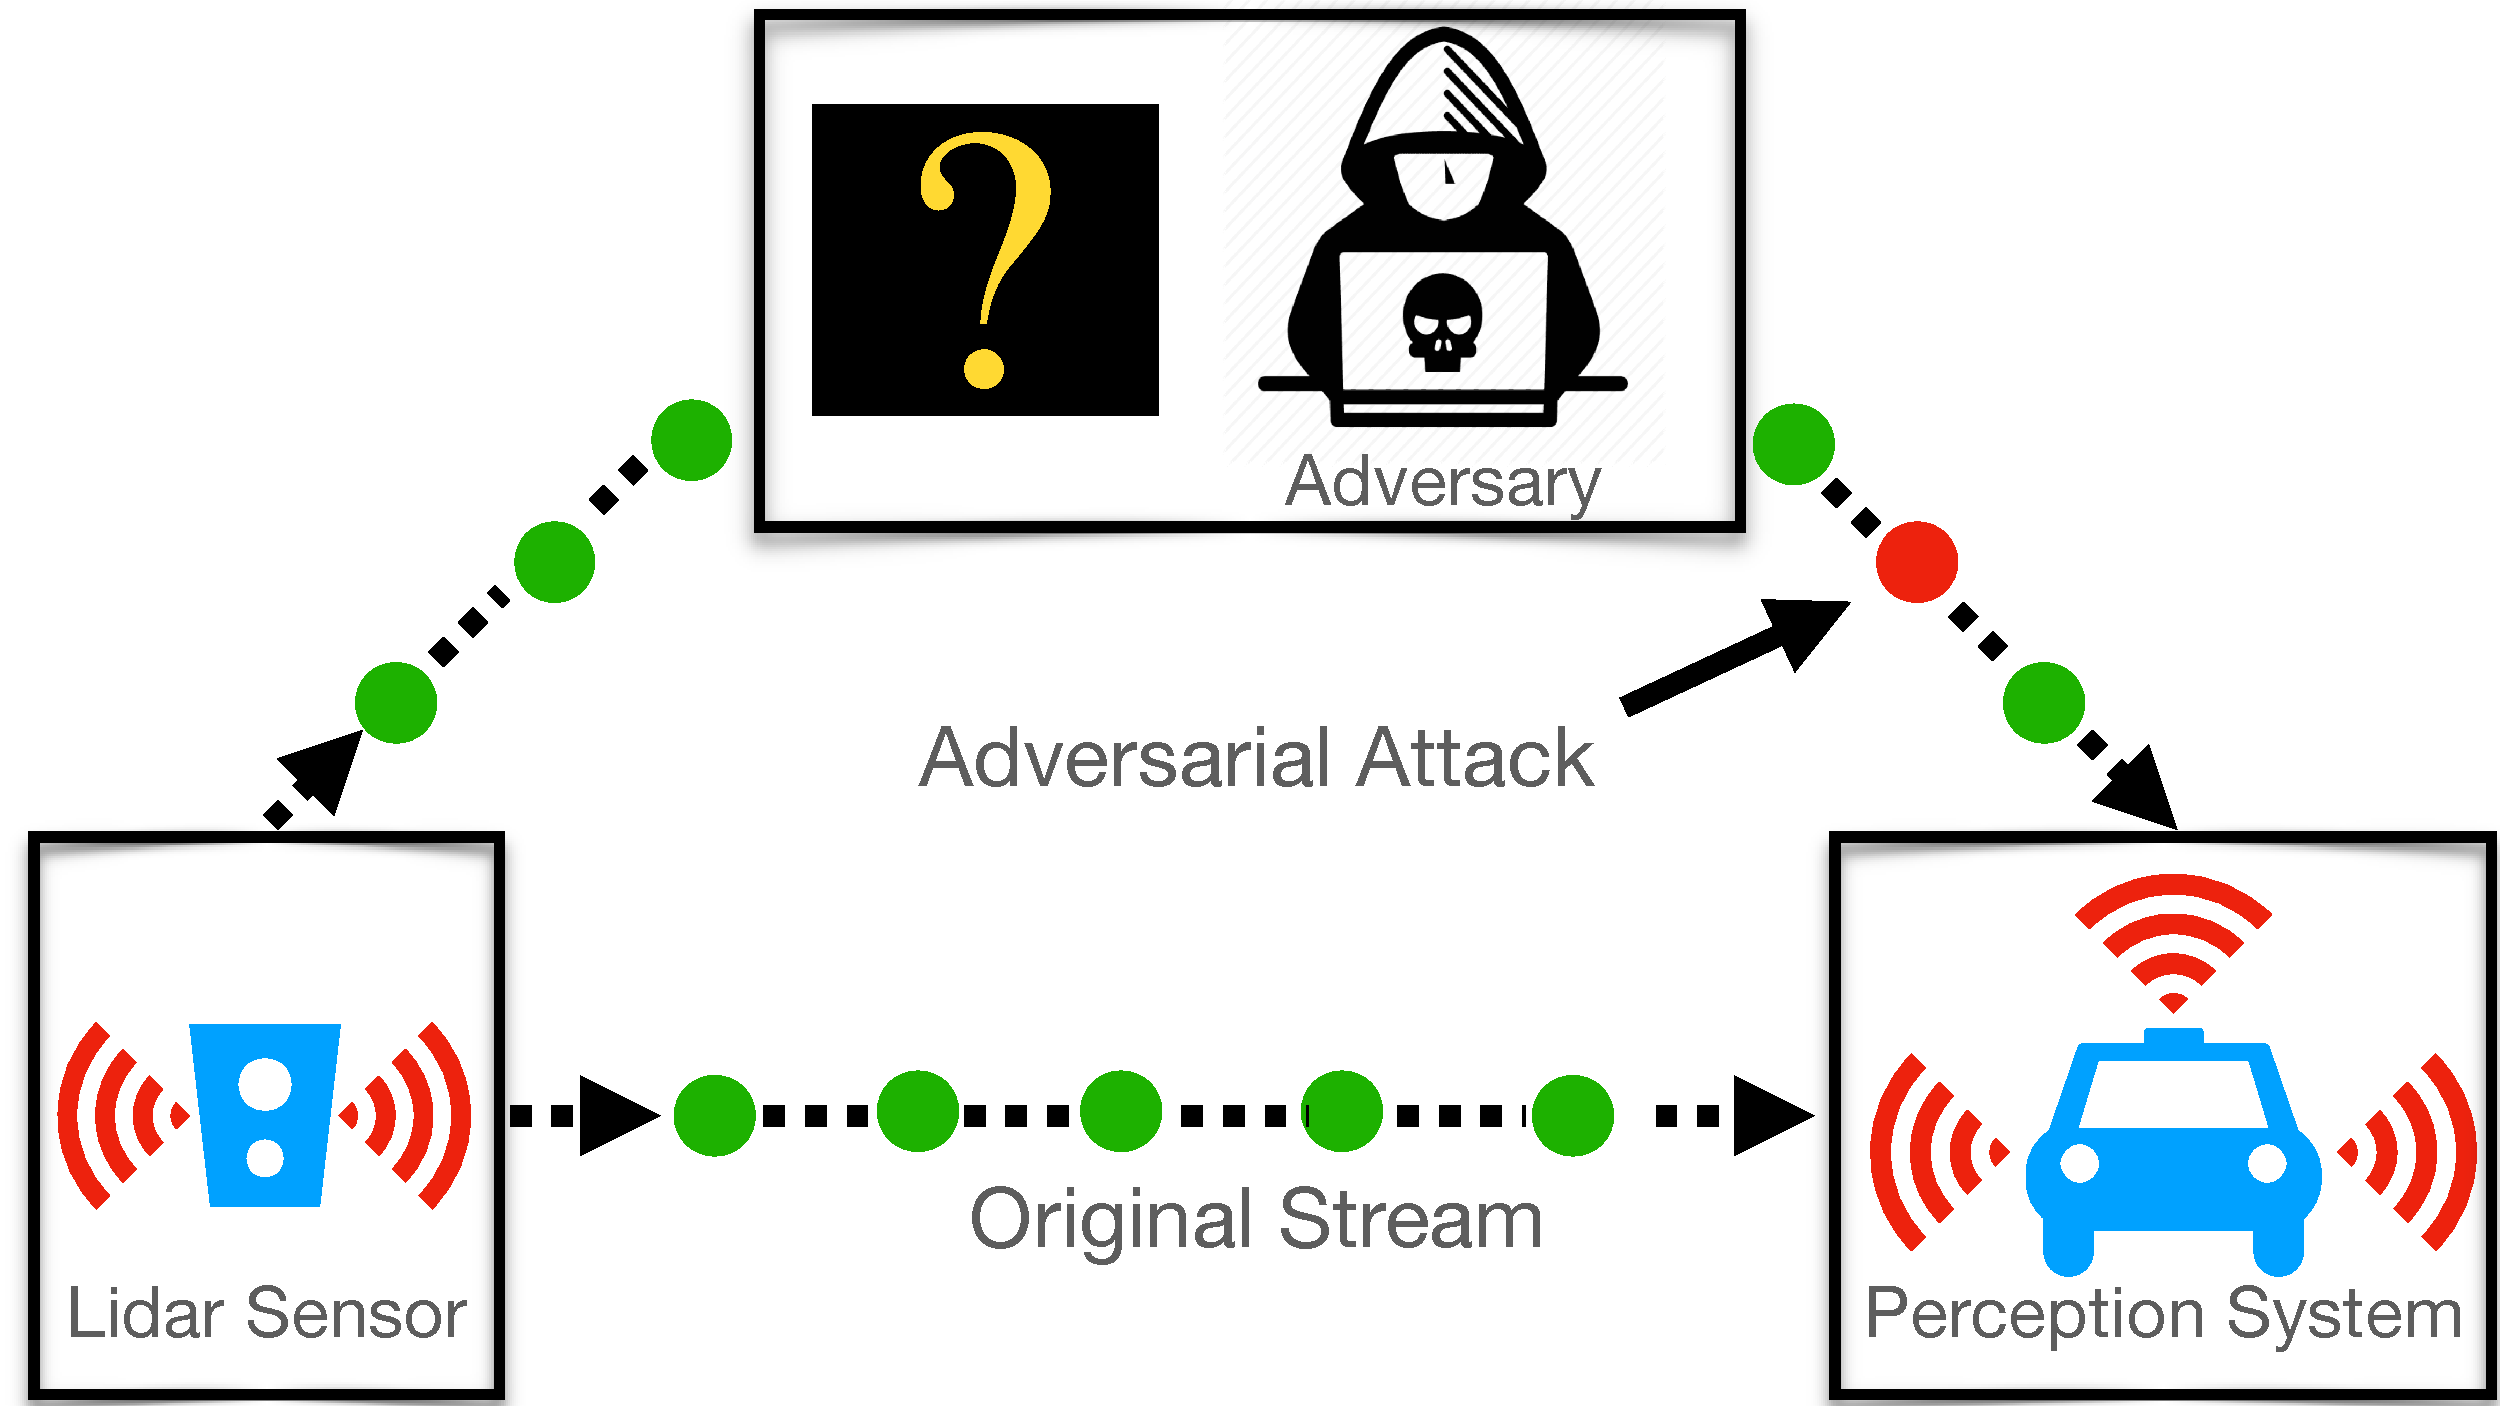
\includegraphics[width=0.38\textwidth]{Figures/man_in_the_middle_attack_2.pdf}
  %\end{center}
  \vspace{-2pt}
\caption{Man-in-the-Middle Attack.}
\label{fig:man_in_the_middle}
\end{wrapfigure}

\begin{enumerate}[noitemsep,topsep=0pt,parsep=0pt,partopsep=0pt, leftmargin=*] 
    \item \textbf{Transiency:} At every time step, the attacker makes an irrevocable decision on whether to attack and if she fails, or opts not to attack, then that datapoint is no longer available for further attacks.
    \item \textbf{Online Attack Budget:} The adversary---to remain anonymous from stateful defences---is restricted to a small selection budget and must optimally balance a passive exploration phase before selecting high value items in the data stream (e.g. easiest to attack) to submit an attack on.
\end{enumerate}

To the best of our knowledge, the only existing approaches that craft adversarial examples on streaming data \citep{gong2019real,lin2017tactics,sun2020stealthy} require multiple passes through a data stream and thus cannot be applied in a realistic online setting where an adversary is forced into irrevocable decisions. Moreover, these approaches do not come with theoretical guarantees. Consequently, assessing the practicality of adversarial attacks---to better expose risks---in a truly online setting is still an open problem, and the focus of this paper. %Our main contributions are the proposal of a new \emph{online threat model} capturing the challenges of the online setting as well as providing a \emph{theoretical framework} (\S\ref{stochastic_k_secretary}) and a \emph{practical algorithm} (Alg.~\ref{alg:online_adv_attack}) to ground the study of online adversarial attacks. 


\xhdr{Main Contributions} 
\looseness=-1
We formalize the online threat model to study adversarial attacks on streaming data. In our online threat model, the adversary must execute $k$ successful attacks within $n$  streamed data points, where $k \ll n$. As a starting point for our analysis, we study the deterministic online threat model in which the actual value of an input---i.e., the likelihood of a successful attack---is revealed along with the input. Our first insight elucidates that such a threat model, modulo the attack strategy, equates to the $k$-secretary problem known in the field of optimal stopping theory \cite{dynkin1963optimum,kleinberg2005multiple}, allowing for the application of established online algorithms for picking optimal data points to attack. We then propose a novel online algorithm \algoname\ that is both practical, simple to implement for any pair $(k,n)$, and requires no additional hyperparameters.%, making it a natural choice for online adversarial attacks.
 

Besides, motivated by attacking blackbox target models, we also introduce a modified secretary problem dubbed the \textit{stochastic $k$-secretary problem}, which assumes the values an attacker observes are stochastic estimates of the actual value. We prove theoretical bounds on the competitive ratio for \emph{any} classical online algorithms in this setting. Guided by our theoretical results, we conduct a suite of experiments on both toy and standard datasets and classifiers (i.e., MNIST and CIFAR-10). Our empirical investigations reveal two counter-intuitive phenomena that are unique to the online blackbox transfer attack setting: 1.) In certain cases attacking robust models may in fact be easier than non-robust models based on the distribution of values observed by an online algorithm. 2.) Simple attack strategies like FGSM can seemingly achieve higher online attack transfer rates than stronger PGD-attackers when paired with a online selection algorithm, demonstrating the importance of carefully selecting which data points to attack. Our key contributions are summarized as follows:

%We empirically show that even simple attack strategies can achieve high attack transfer rates when paired with an online algorithm, demonstrating the importance of carefully selecting which data points to attack.


\begin{itemize}[noitemsep,topsep=0pt,parsep=0pt,partopsep=0pt,label={\large\textbullet},leftmargin=*]
\item We formalize the online adversarial attack threat model as an online decision problem and rigorously connect it to a generalization of the k-secretary problem.
\item We introduce and analyze \algoname, an extension of \textsc{Virtual} for the $k$-secretary problem yielding a significant practical improvement ($60\%$). %over \textsc{Virtual}. 
% and analytically derive a tight lower bound to the competitive ratio for \emph{general}-$k$.
% \item We propose a modification of the \textsc{Virtual} algorithm for the $k$-secretary problem that yield 
We then provide, via novel techniques, a tractable formula for its competitive ratio, partially answering one of \citet{albers2020new}'s open questions (see footnote~\footref{foot:closed_form}) and achieving a new state-of-the-art competitive ratio for $k<5$.
\item We propose Alg.~\ref{alg:online_adv_attack} that leverages (secretary) online algorithms to perform efficient online adversarial attacks. We compare different online algorithms including \algoname\ via experiments on MNIST and CIFAR-10 in the challenging Non-Interactive BlackBox transfer (NoBox) setting.% and show that in many cases our onilne algorithm performs almost as well as an offline algorithm.
\end{itemize}

%competitive ratio for $k<5$ among all single threshold algorithms. \cut{Our proof technique also closes the open question in ~\citet{babaioff2007knapsack} by extending the competitive analysis to the general $k$-regime of the original \textsc{Virtual} algorithm to \algoname\ by removing theoretically convenient constraints. }
\section{Background and Preliminaries}
\looseness=-1
\vspace{-5pt}
% We first briefly review the classical adversarial attack setup and the $k$-secretary problem that serve as foundations for the online threat model outlined later in \S\ref{online_adversarial_attacks}.

\xhdr{Classical Adversarial Attack Setup}
We are interested in constructing adversarial examples against some fixed 
target classifier $f_{t}: \mathcal{X} \to \mathcal{Y}$ which consumes input data points $x \in \mathcal{X}$ and labels them with a class label $y \in \mathcal{Y}$. The goal of an adversarial attack is then to produce an adversarial example $x' \in \mathcal{X}$, such that $f_t(x') \neq y$, and where the distance $d(x,x') \leq \gamma$. Then, equipped with a loss $\ell$ used to evaluate $f_{t}$, an attack is said to be optimal if \citep{carlini2017magnet, madry2017towards}, 
\begin{equation}\label{eq:opt_attack}
    \textstyle x' \in \argmax_{x'\in \gX}\ell(f_{t}(x'),y) \,, \;\; \text{s.t.} \;\; d(x,x') \leq \gamma \,.
\end{equation}
Note that the formulation above makes no assumptions about access and resource restrictions imposed upon the adversary. Indeed, if the parameters of $f_t$ are readily available, we arrive at the familiar whitebox setting, and problem in \eqref{eq:opt_attack} is solved by following the gradient $\nabla_x f_{t}$ that maximizes $\ell$. 

\xhdr{k-Secretary Problem}
The secretary problem is a well-known problem in theoretical computer science \cite{dynkin1963optimum,ferguson1989solved}. Suppose that we are tasked with hiring a secretary from a randomly ordered set of $n$ potential candidates to select the secretary with maximum value. The secretaries are interviewed sequentially and reveal their actual value on arrival. Thus, the decision to accept or reject a secretary must be made immediately, irrevocably, and without knowledge of future candidates. While there exist many generalizations of this problem, in this work, we consider one of the most canonical generalizations known as the \textit{$k$-secretary problem} \cite{kleinberg2005multiple}. Here, instead of choosing the best secretary, we are tasked with choosing $k$ candidates to maximize the expected sum of values. Typically, online algorithms that attempt to solve secretary problems are evaluated using the competitive ratio, which is the value of the objective achieved by an online algorithm compared to an optimal value of the objective that is achieved by an ideal ``offline algorithm,” i.e., an algorithm with access to the entire candidate set. Formally, an online algorithm $\mathcal{A}$ that selects a subset of items $S_{\mathcal{A}}$  is said to be $C$-competitive to the optimal algorithm $\textrm{OPT}$ which greedily selects a subset of items $S^*$ while having full knowledge of all $n$ items, if asymptotically in $n$
\begin{equation}
    \mathbb{E}_{\pi\sim \mathcal{S}_n}[\setvaluemath(S_{\mathcal{A}})] \geq  (C + o(1)) \setvaluemath(S^*) \,,
    \label{eq:comp_ration}
\end{equation}
where \setvalue\ is a set-value function that determines the sum utility of each algorithm's selection, and the expectations are over permutations sampled from the symmetric group of $n$ elements, $\mathcal{S}_n$, acting on the data. In \S\ref{stochastic_k_secretary}, we shall further generalize the $k$-secretary problem to its stochastic variant where the online algorithm is no longer privy to the actual values but must instead choose under uncertainty.

\cut{
\begin{equation*}
    \mathbb{E}_{\pi\sim \mathcal{S}_n}[\setvaluemath(S_{\mathcal{A}})] \geq  (C + o(1)) \setvaluemath(S^*) \,.
    \label{eq:asym_omp_ration}
\end{equation*}
}



\cut{--along with an accompanying definition of a stochastic competitive ratio---}
\section{Online Adversarial Attacks}
\label{online_adversarial_attacks}

Motivated by our more realistic threat model, we now consider a novel adversarial attack setting where the data is no longer static but arrives in an online fashion.

\subsection{Adversarial Attacks as Secretary Problems}
\label{adv_sec_problem}
The defining feature of the online threat model---in addition to streaming data and the fact that we may not have access to the target model $f_t$---is the online attack budget constraint.
Choosing when to attack under a fixed budget in the online setting can be related to a secretary problem. We formalize this online adversarial attack problem in the boxed online threat model below.

In the online threat model we are given a data stream $\mathcal{D}=\{(x_1,y_1),\ldots,(x_n,y_n)\}$ of $n$ samples ordered by their time of arrival. In order to craft an attack against the target model $f_t$, the adversary selects, using its online algorithm $\mathcal{A}$, a subset $S_{\mathcal{A}} \subset \mathcal{D}$ of items to maximize: %\footnote{$S_{\mathcal{A}}$ contains either indexes or elements of the datastream.}
\begin{equation}\label{eq:asp}
   \setvaluemath(S_\mathcal{A}) \! := \!\!\! \sum_{ (x,y) \in S_\mathcal{A}} \ell(f_{t}(\textsc{Att}(x)),y) \ \text{ s.t. } 
   |S_A| \leq k,\hspace{-1mm} 
\end{equation}
\cut{
\begin{equation}\label{eq:asp}
   \setvaluemath(S_\mathcal{A}) \! := \!\!\! \sum_{ i \in S_\mathcal{A}}v_i \text{ s.t. }  v_i = \ell(f_{t}(x_i'),y_i) \text{ and }
   |S_A| \leq k,\hspace{-1mm} 
\end{equation}
}
where $\textsc{Att}(x)$ denotes an attack on $x$ crafted by a \emph{fixed} attack method $\textsc{Att}$ that might or might not depend on $f_t$. From now on we define $x_i'=\textsc{Att}(x_i)$. 
Intuitively, the adversary chooses $k$ instances that are the ``easiest" to attack, i.e. samples with the highest value. Note that selecting an instance to attack does not guarantee a successful attack.
Indeed, a successful attack vector may not exist if the perturbation budget $\gamma$ is too small. \cut{even though the value is maximized.} However, stating the adversarial goal as maximizing the value of $S_{\mathcal{A}}$ leads to the measurable objective of calculating the ratio of successful attacks in $S_{\mathcal{A}}$ versus $S^*$.

If the adversary knows the true value of a datapoint then the online attack problem reduces to the original $k$-secretary. On the other hand, the adversary might not have access to $f_t$ and instead, the adversary's value function may be an estimate of the true value---e.g.\ the loss of a surrogate classifier, and the adversary must make selection decisions in the face of uncertainty.\cut{ yielding a stochastic generalization of the $k$-secretary problem.} The theory developed in this paper will tackle both the case where values $v_i:=\ell(f_t(x_i'),y_i)$ for $i \in \{1,\ldots,n\} :=[n]$ are known (\S\ref{virtual_plus}), as well as the richer stochastic setting with only estimates of $v_i\,,\, i \in [n]$ (\S\ref{stochastic_k_secretary}).


\xhdr{Practicality of the Online Threat Model} It is tempting to consider whether in practice the adversary should forego the online attack budget and instead attack every instance. However, such a strategy poses several critical problems when operating in real world online attack scenarios. Chiefly, attacking any instance in $\mathcal{D}$ incurs a non-trivial risk that the adversary is detected by a defense mechanism. Indeed, when faced with stateful defence strategies (e.g. \cite{chen2020stateful}) every additional attacked instance further increases the risk of being detected and rendering future attack impotent. Moreover, attacking every instance may be infeasible computationally for large $n$ or impractical based on other real-world constraints. Generally speaking, as conventional adversarial attacks operate by restricting the perturbation to a fraction of the maximum possible change (e.g., $\ell_{\infty}$-attacks) online attacks analogously restrict the time window to a fraction of possible instances to attack. Similarly, knowledge of $n$ is also a factor that the adversary can easily control in practice. For instance, in the autonomous control system example the adversary can choose to be active for a short interval---e.g., when the autonomous car is a certain geospatial location---and thus set the value for $n$.

\begin{ftheo}
The online threat model relies on the following key definitions:
\begin{itemize}[leftmargin=*, itemsep=1pt, topsep=1pt, parsep=1pt]
\item 
\textbf{The target model $f_t$}. The adversarial goal is to attack some target model $f_t : \mathcal{X} \rightarrow \mathcal{Y}$, through adversarial examples that respect a chosen distance function, $d$, with tolerance $\gamma$. %--i.e. $d(x,x') \leq \gamma$ 

\item
\textbf{The data stream $\mathcal{D}$}. The data stream $\mathcal{D}$ contains the $n$ examples $(x_i,y_i)$ ordered by their time of arrival. At any timestep $i$, the adversary receives the corresponding item in $\mathcal{D}$ and must decide whether to execute an attack or forever forego the chance to attack this item.

\item
\textbf{Online attack budget $k$}. The adversary is limited to a maximum of $k$ attempts to craft attacks within the online setting thus imposing that each attack is on a unique item in $\mathcal{D}$.

\item
\textbf{A value function $\mathcal{V}$}. Each item in the dataset is assigned a value on arrival by the value function $\mathcal{V}: \mathcal{X} \times \mathcal{Y} \rightarrow \mathbb{R}_+$ which represents the utility of selecting the item to craft an attack. This can be the likelihood of a successful attack under $f_t$ (true value) or a stochastic estimate of the incurred loss given by a surrogate model $f_s \approx f_t$.
\end{itemize}

The online threat model corresponds to the setting where the adversary seeks to craft adversarial attacks (i) against a target model $f_t \in \gF$, (ii) by observing items in $\mathcal{D}$ that arrive online, (iii) and choosing $k$ optimal items to attack by relying on (iv) an available value function $\mathcal{V}$. The adversary's objective is then to use its value function towards selecting items in $\mathcal{D}$ that maximize the sum total value of selections \setvalue\ (Eq.~\ref{eq:asp}).
\end{ftheo}


\subsection{\algoname\ for Adversarial Secretary Problems}
\label{virtual_plus}
Let us first consider the deterministic variant of the online threat model, where the true value is known on arrival. For example consider the value function $\mathcal{V}(x_i,y_i) = \ell(f_{t}(x'_i),y_i) = v_i$ i.e. the loss resulting from the adversary corrupting incoming data $x_i$ into $x'_i$. Under a fixed attack strategy, the selection of high-value items from $\mathcal{D}$ is exactly the original $k$-secretary problem and thus the adversary may employ any $\mathcal{A}$ that solves the original $k$-secretary problem.

%\setlength{\textfloatsep}{5pt}% Remove \textfloatsep

\begin{minipage}[t]{.49\textwidth}
\vspace{-15pt}
\begin{algorithm}[H]
\small
\textbf{Inputs:} $t\in[k\dots n-k]$, $R = \emptyset$, $S_{\mathcal{A}} = \emptyset$
\newline
\textbf{Sampling phase:} Observe the first $t$ data points and construct a sorted list $R$ with the indices of the top $k$ data points seen. The method $\texttt{sort}$ ensures: $ \mathcal{V}(R[1]) \geq \mathcal{V}(R[2]) \dots \geq \mathcal{V}(R[k]).$
\newline
\textbf{Selection phase}:{\color{salmon} \{//\textsc{Virt}+ removes L2-3 and adds L4 \}} \hspace{-4.0cm}% and adds a condition  L4\}} \hspace{-3cm}
\begin{algorithmic}[1]
\FOR{$i:=t+1$ to $n$ }
    % \newline
    % {\hspace*{-0.5cm}\color{salmon} \small \COMMENT{// \algoname removes lines 5-6 from \textsc{Virtual}}}
    \IF{$\mathcal{V}(i) \geq \mathcal{V}(R[k])$ and $R[k] > t$}
        \STATE $R$ = $\texttt{sort}(R \cup \{i\} \setminus \{R[k]\})$
        \hfill  
        % \{// Update $R$\}
        \tikzmark{start}
        \tikzmark{stop}
        \begin{tikzpicture}[remember picture, overlay]
        \draw[salmon,thick] ([xshift=-155pt,yshift=13pt]pic cs:start) -- ([xshift=-20pt, yshift=12pt]pic cs:stop);        \draw[salmon,thick] ([xshift=-155pt,yshift=2pt]pic cs:start) -- ([xshift=-20pt, yshift=2pt]pic cs:stop);
         \draw[salmon,thick] ([xshift=-155pt,yshift=-8pt]pic cs:start) -- ([xshift=-142pt, yshift=-8pt]pic cs:stop);
        \end{tikzpicture}
    %\tikzmk{A}
    \tikzmark{start1}
    \tikzmark{stop2}
    \begin{tikzpicture}[remember picture, overlay]
    \end{tikzpicture}
    \ELSIF {$\mathcal{V}(i) \geq \mathcal{V}(R[k])$ {\color{salmon} and $ |S_{\mathcal{A}}| \leq  k$} }
    \STATE $R$ = $\texttt{sort}(R \cup \{i\} \setminus \{R[k]\})$ \hfill\COMMENT{// Update $R$}
    \STATE $S_{\mathcal{A}} = S_{\mathcal{A}} \cup \{i \}$ \hfill\COMMENT{// Select element $i$}
    \ENDIF
    %\tikzmk{B}
    %\boxit{pink}
%\STATE
\ENDFOR
\end{algorithmic}
 \caption{\small \textsc{Virtual} and {\color{salmon}\algoname\,} }
 \label{alg:virtual_plus}
\end{algorithm}
\end{minipage}
\hfill
\begin{minipage}[t]{.48\textwidth}
\begin{figure}[H]
 \vspace{-15pt}
    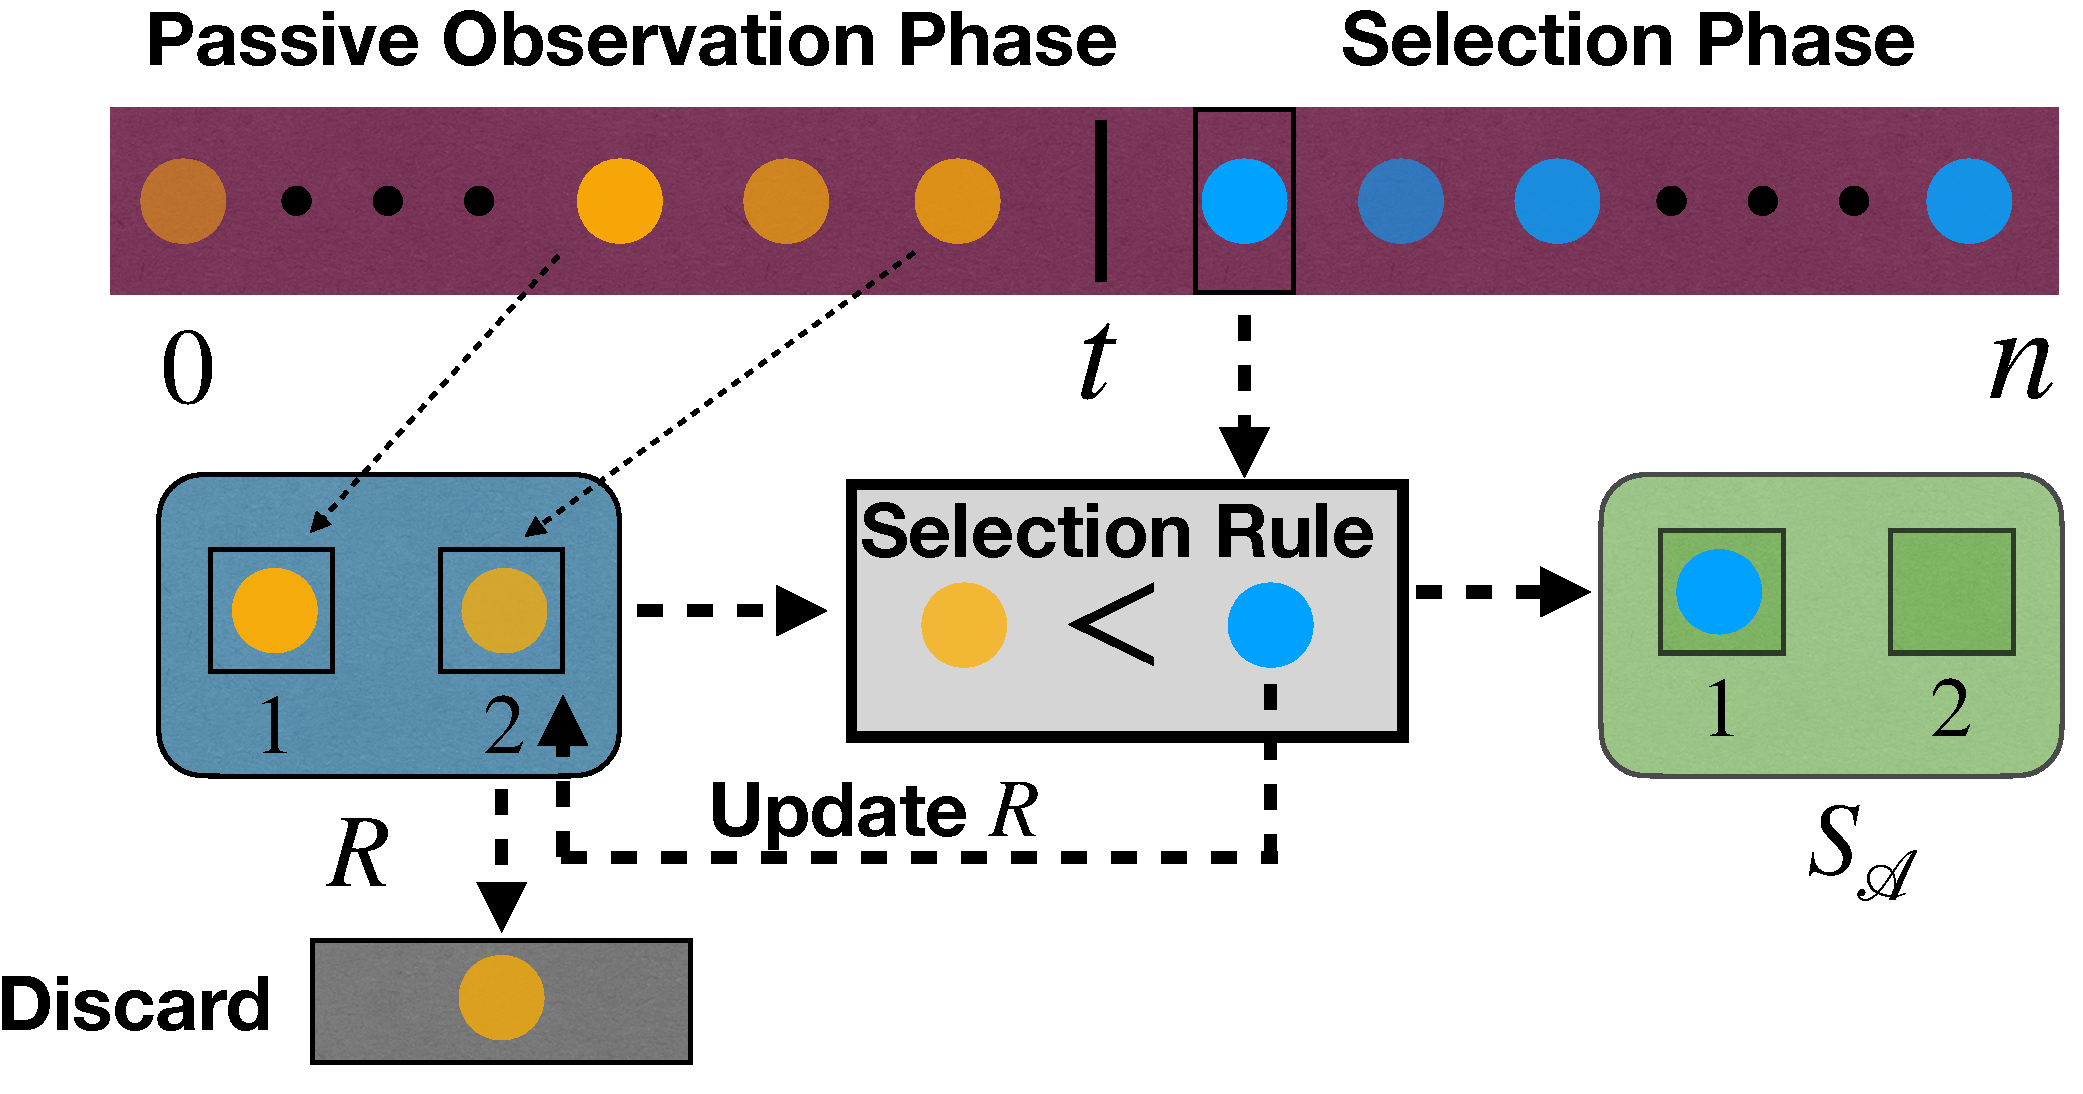
\includegraphics[width=1.01\linewidth]{Figures/Virtual+_algo.pdf}
    \vspace{-10pt}
    \caption{\algoname \ observes $v_i$ (or estimates) and maintains $R$ during the sampling phase. Items are then picked into $S_{\mathcal{A}}$, after threshold $t$, \cut{via comparisons to $R$.}}
    \label{fig:stochastic_secretary}
\end{figure}
\end{minipage}
\cut{
\begin{minipage}[t]{.48\textwidth}
\vspace{0pt}  
    \begin{algorithm}[H]
    \small
    \textbf{Inputs:} Permuted Datastream: $\mathcal{D}_\pi$, Online Algorithm: $\mathcal{A}$,  Surrogate classifier: $f_s$, Target classifier: $f_t$,  Attack method: \textsc{Att}, Loss: $\ell$,  Budget: $k$,  
    Fool rate: $F^{\mathcal{A}}_\pi=0$.
    \begin{algorithmic}[1]
    \FOR{$(x_i,y_i)$ in $\mathcal{D}_\pi$}
    \STATE $x_i' \leftarrow  \textsc{Att}(x_i)$ \hfill \COMMENT{// Compute the attack}
    \STATE $\mathcal{V}_i \leftarrow \ell(f_s(x_i'),y_i)$  \hfill \COMMENT{// Compute the estimate of $v_i$}
    \IF{$\mathcal{A}(\mathcal{V}_1,\ldots, \mathcal{V}_i,k) == \textsc{True}$}
    \STATE  $F^{\mathcal{A}}_\pi \leftarrow F^{\mathcal{A}}_\pi+\tfrac{\mathbf{1}\{f_t(x_i')\neq y_i\}}{k}$  \hfill\COMMENT{// Submit  $x_i'$ on $f_t$} 
    \ENDIF
    \ENDFOR
    \STATE \textbf{return:} $F^{\mathcal{A}}_\pi$ \hfill\COMMENT{// Note that $\mathcal{A}$ always submits $k$ attacks} 
    \end{algorithmic}
     \caption{\small Online Adversarial Attack}
     \label{alg:online_adv_attack}
    \end{algorithm}
\end{minipage}
}


Well known single threshold-based algorithms that solve the $k$-secretary problem include the \textsc{Virtual}, \textsc{Optimistic} \cite{babaioff2007knapsack} and the recent \textsc{Single-Ref} algorithm \cite{albers2020new}. In a nutshell, these online algorithm consists of two phases---a \textit{sampling phase} followed by a \textit{selection phase}---and an optimal stopping point $t$ (threshold) that is used by the algorithm to transition between the phases. In the sampling phase, the algorithms passively observe all data points up to a pre-specified threshold $t$. Note that $t$ itself is algorithm-specific and can be chosen by solving a separate optimization problem. Additionally, each algorithm also maintains a sorted reference list $R$ containing the top-$k$ elements. Each algorithm then executes the selection phase through comparisons of incoming items to those in $R$ and possibly updating $R$ itself in the process (see~\S\ref{appendix:classical_online_algorithms}).

Indeed, the simple structure of both the \textsc{Virtual} and \textsc{Optimistic} algorithms---e.g., having few hyperparameters and not requiring the algorithm to involve Linear Program's for varying values of $n$ and $k$---in addition to being $(1/e)$-competitive (optimal for $k=1$) make them suitable candidates for solving \eqref{eq:asp}. However, 
the competitive ratio of both algorithms in the small $k$ regime---but not $k=1$---has shown to be sub-optimal with \textsc{Single-Ref} provably yielding larger competitive ratios at the cost of an additional hyperparameter selected via combinatorial optimization when $n \to \infty$. 

We now present a novel online algorithm \algoname\ that retains the simple structure of \textsc{Virtual} and \textsc{Optimistic}, with no extra hyperparameters, but leads to a new state-of-the-art competitive ratio for $k<5$. Our key insight is derived from re-examining the selection condition in the \textsc{Virtual} algorithm and noticing that it is overly conservative and can be simplified. The \algoname\ algorithm is presented in Algorithm 1, where the removed condition in \textsc{Virtual} (L2-3) is \st{in pink strikethrough}. Concretely, the condition that is used by \textsc{Virtual} but \emph{not} by \algoname\ updates $R$ during the selection phase without actually picking the item as part of $S_{\mathcal{A}}$. Essentially, this condition is theoretically convenient and leads to a simpler analysis by ensuring that the \textsc{Virtual} algorithm never exceeds $k$ selections in $S_{\mathcal{A}}$. \algoname\ removes this conservative $R$ update criteria in favor of a simple to implement condition, $|S_{\mathcal{A}}| \leq k$ line 4 {\color{salmon}(in pink)}. Furthermore, the new selection rule also retains the simplicity of \textsc{Virtual} leading to a painless application to online attack problems.

\cut{By design, \algoname\ also does not exceed $k$ selections and works for any combination of $k$ and $n$.}
\xhdr{Competitive ratio of \algoname}
What appears to be a minor modification in \textsc{Virtual+} compared to \textsc{Virtual} leads to a significantly more involved analysis but a larger competitive ratio. In Theorem 1, we derive the analytic expression that is a tight lower bound for the competitive ratio of \algoname\ for \emph{general}-$k$. We see that \algoname\ provably improves in competitive ratio for $k<5$ over both \textsc{Virtual}, \textsc{Optimistic}, and in particular the previous best single threshold algorithm, \textsc{Single-Ref}.

\begin{theorem}
The competitive ratio of Virtual Plus for the case $k \geq 2$ where $t = \alpha n$ can asymptotically be lower bounded by 
\begin{equation}
    C_k \geq  \max_{\alpha \in [0,1]}  {\alpha}^k \sum_{m = 0}^{k - 1} a_m \ln^m (\alpha)- \alpha a_0
    \quad where  \quad
    a_m := \big(\tfrac{k^k}{(k-1)^{k-m}} - k^m\big)\frac{(-1)^{m+1}}{m!}
    \, .
\end{equation}
Particularly, we get $C_2\geq0.427, C_3\geq .457, C_4\geq.4769$ outperforming~\citet{albers2020new}.
\label{thm:K_2_theorem1}
\end{theorem}

\cut{
\begin{theorem}
The competitive ratio of \algoname \ for the case $k \geq 2$ and where $t = \alpha \cdot n$ can asymptotically be lower bounded by: 
\begin{equation}
    C_k >  \max_{\alpha \in [0,1]}  {\alpha}^k \left (\sum_{m = 0}^{k - 1} a_m \ln^m (\alpha)\right) - \alpha a_0
\end{equation}
    where 
\begin{equation}
    a_m = \sum_{a = m}^{k - 1} \left (\frac{k}{k - 1}\right)^a \frac{(k - 1)^{m - 1}}{m!}(-1)^{m + 1}
    \, .
\end{equation}
For example when $k=2$ asymptotically we have,
% \vspace{-1mm}
\begin{equation}
    C \geq  \max_{\alpha \in [0,1]} \alpha ( 3(1-\alpha) + 2 \alpha \ln(\alpha)) > .4273 > 1/e \, .
\end{equation}
\label{thm:K_2_theorem1}
\end{theorem}
}
\cut{
\begin{theorem} For $k=2$, $t= \alpha n\,,\, \alpha \in (0,1)$, the competitive ratio achieved by \algoname\ follows,

% \begin{equation}
% % \textstyle
%     C_n = \frac{t(t+1)}{n} \sum_{j=t+1}^n\tfrac{1}{j(j+1)} \Big(1 + 2 \sum_{p=t+1}^j \tfrac{1}{p-1}\Big)
% \end{equation}
% Particularly for  we get 
% \vspace{-1mm}
\begin{equation} \label{eq:lower_bound_alpha}
    C \geq \alpha ( 3(1-\alpha) + 2 \alpha \ln(\alpha)) + \mathcal{O}(1/n)
    % \vspace{-1mm}
\end{equation}
Thus, asymptotically  we have
% \vspace{-1mm}
\begin{equation}
    C \geq  \max_{\alpha \in [0,1]} \alpha ( 3(1-\alpha) + 2 \alpha \ln(\alpha)) > .4273 > 1/e \, .
\end{equation}
% \vspace{-6mm}
\label{thm:K_2_theorem1}
\end{theorem}
}
% \begin{proof}[Proof sketch]
% The full proof can be found in \S\ref{appendix:virtual_plus_proof_k_2}. First note that by~\citep[Lem.~3.3]{albers2020new}, we have a competitive ratio for the $k$-secretary problem under any threshold-based algorithm that is equal to 
% \begin{equation}
%   C_n = \tfrac{1}{k}(\mathbb{P}(i_1 \in S_{\mathcal{A}}) + \ldots + \mathbb{P}(i_k \in S_{\mathcal{A}})) \label{eq:C_as_sum_prob}
% \end{equation}
% where $i_a$ is the index of the $a^{th}$ best secretary. 
% Now, let us focus on the case $k=2$.
% When calculating the probability of one of the top-$2$ elements being picked by the algorithm, we must calculate the probability of one of the top-2 elements being picked after the threshold ---i.e., for a given time step $j+1$ between $t+1 \dots n$. A top-$2$ element is picked by \algoname\ if and only if this element appears at that time step and if we haven't already picked $2$ secretaries ($|S_{\mathcal{A}}| < 2$) during the first $j$ steps. Thus, for $a \in \{1,2\}$,
% \begin{align}
%     \mathbb{P}(i_a \in S_{\mathcal{A}}) 
%     % &= \sum_{j=t+1}^n \mathbb{P}(i_a \in S_{\mathcal{A}} \ \text{at time-step }j)  \\
%     &= \tfrac{1}{n}\left(\mathbb{P}_t(|S_{\mathcal{A}}| < 2) +\ldots+ \mathbb{P}_{n-1}(|S_{\mathcal{A}}| < 2)\right)\label{p_picked_equal_not_filled} \notag
% \end{align}
% where $\mathbb{P}_j(E):= \mathbb{P}(E \ \text{in first } j \text{ steps})$ for any event $E$.
% Now, for a given $j$, we compute $\mathbb{P}_j(|S_{\mathcal{A}}| < 2)$ by decomposing the event into the probability of having an empty $S_{\mathcal{A}}$ plus the probability of having $|S_{\mathcal{A}}| = 1$. The computation of the latter is detailed in \S\ref{appendix:virtual_plus_proof_k_2} and summarized in Fig.~\ref{fig:k_2}.
% %\vspace{-1mm}
% \begin{align}
%     \mathbb{P}_j(|S_{\mathcal{A}}| \!=\! 0)
%     =  \tfrac{t(t - 1)}{j (j - 1)},\,
%     \mathbb{P}_j(|S_{\mathcal{A}}| \!=\! 1)
%     = \tfrac{2t}{j(j-1)} \sum_{p = t + 1}^{j}\tfrac{t-1}{p-2} \notag
% %\vspace{-1mm}
% \end{align}
% Overall, by combining the previous equations we get:
% %\vspace{-1mm}
% \begin{equation}
%     C_n = \frac{1}{n}\sum_{j=t}^{n-1}\Big( \frac{t(t - 1)}{j (j - 1)} + 2 \sum_{p = t + 1}^{j}\frac{1}{j}\frac{t}{j - 1}\frac{t-1}{p-2}\Big)
% %\vspace{-1mm}
% \end{equation}
% % \begin{figure}[t]
% %     \centering
% %     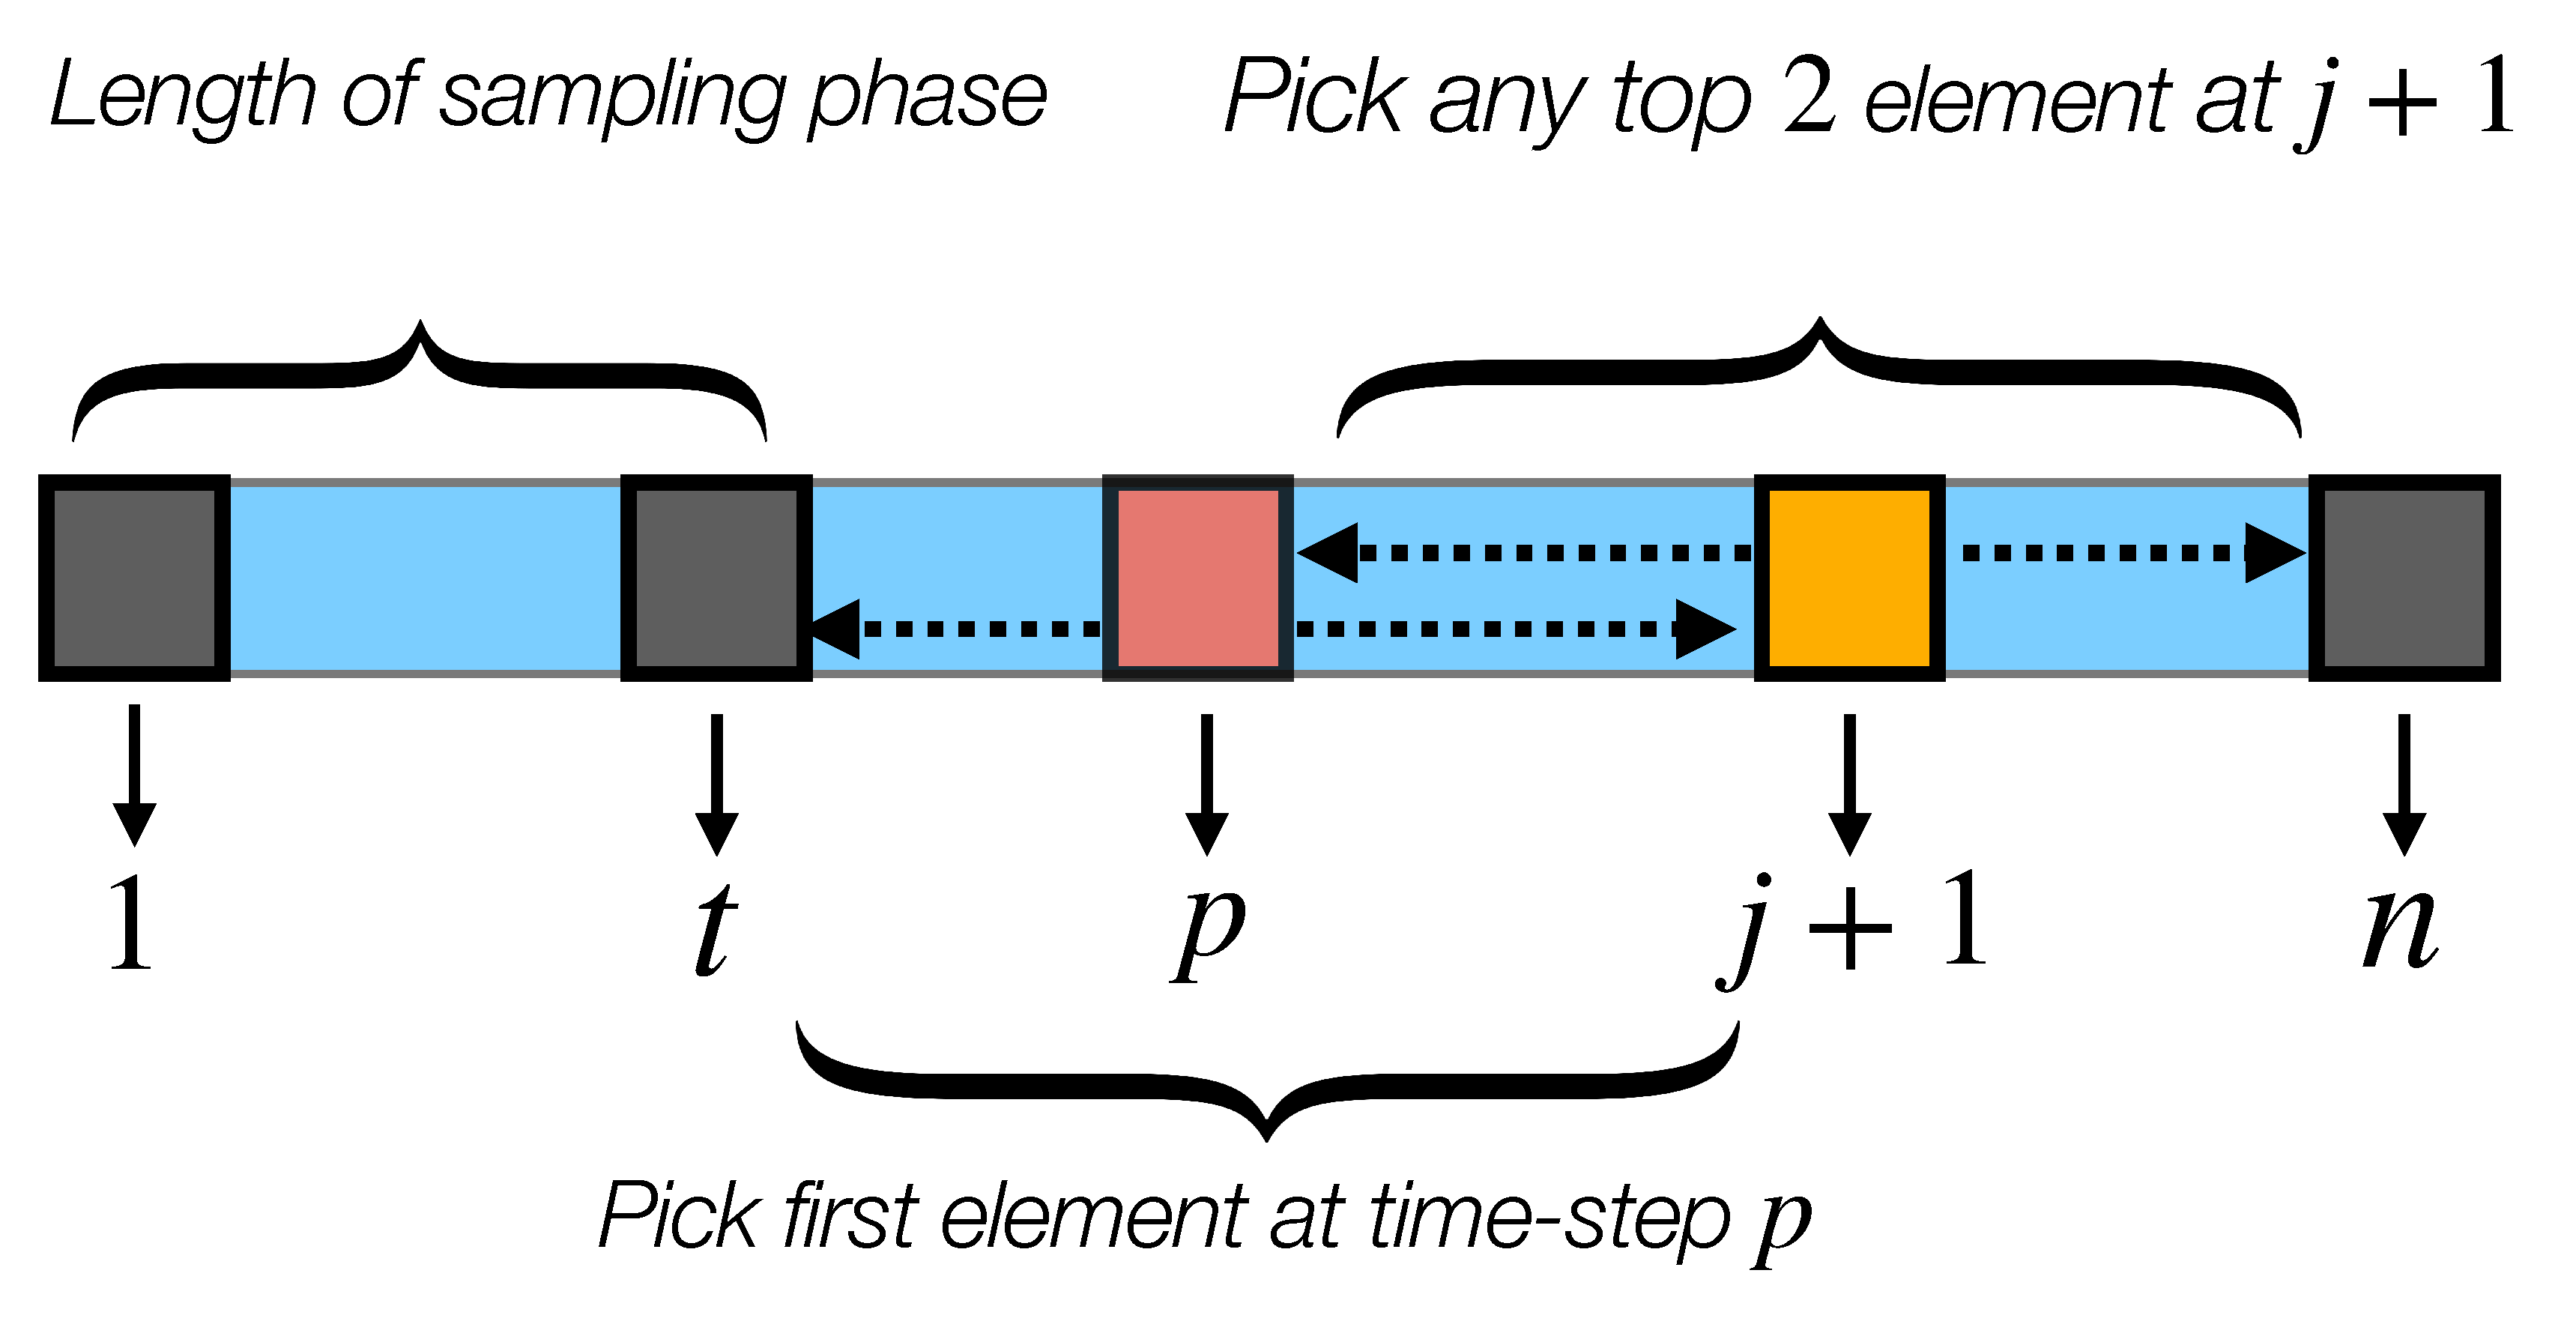
\includegraphics[width=.95\linewidth]{Figures/virtual_plus_k_2.pdf}
% %     \vspace{-15pt}
% %     \caption{Probability of having only one element in $S_{\mathcal{A}}$ after $j$ time-steps with the \algoname algorithm.}
% %     \label{fig:k_2_main}
% %     \vspace{-10pt}
% % \end{figure}
% Finally, by lower bounding the sums with integrals we get, 
% \begin{align}
%     C_n \geq 
%     \tfrac{t(t -1)}{n} \left(\tfrac{3}{t}-\tfrac{2\ln(n/t) + 3}{n} - 2(n-t) \left| \tfrac{16}{3 t^3 e^4} \right|\right) \notag
% %\vspace{-1mm}
% \end{align}
% Now, for $t = \alpha n$ with $\alpha \in (0, 1)$, that lower-bound becomes
% %\vspace{-3mm}
% \begin{equation}
% \label{eq:alpha_eqn}
% C \geq \alpha (3 - \alpha(3 - 2\ln (\alpha))) + \mathcal{O}(1/n) \,,\quad \forall \alpha \in (0,1)
% \end{equation}
% The constant term of the RHS is a concave function of $\alpha$ that is maximized for $\alpha^* \approx 0.38240$. Thus, our algorithms achieves a competitive ratio larger than $0.42737$.
% \end{proof}

\xhdr{Connection to Prior Work}
\label{connection_to_prior_work}
Theorem~\ref{thm:K_2_theorem1} gives a tractable way to compute the competitive ratio of \algoname\ for any $k$, that improve the previous state-of-the-art~\citep{albers2020new} in terms of single threshold $k$-secretary algorithms for $k<5$ and $k>100$.\footnote{\label{foot:closed_form}\citet{albers2020new} only provide competitive ratios of \textsc{Single-Ref} for $k \leq 100$. In their conclusion mentions that ``a closed formula for the competitive ratio for any value
of $k$ is one direction of future work''. We partially answer this open question by expressing \algoname's optimal threshold as the solution of a uni-dimensional optimization problem. In Table~\ref{tab:C_k}, we provide this threshold for a wide range of $k \geq 100$.} 
However, it is also important to contextualize \algoname\ against recent theoretical advances in this space. 
Most prominently, \citet{buchbinder2014secretary} and \citet{chan2014revealing} proved that the $k$-secretary problem can be solved {\em optimally} (in terms of competitive ratio) using linear programs (LPs), {\em assuming a fixed length of $n$}. But these optimal algorithms are typically not feasible in practice.
Critically, they require individually tuning multiple thresholds by solving a separate LP with $\Omega(n k^2)$ parameters for each length of the data stream $n$, and the number of constraints grows to infinity as  $n\rightarrow\infty$. 
In this work, we chose to focus on practical methods with a \emph{single} threshold (e.g. Algorithm~\ref{alg:virtual_plus} or \textsc{Single-Ref}~\citep{albers2020new}) that do not require involved computations that grow with $n$. 




\section{Stochastic Secretary Problem}
\label{stochastic_k_secretary}
\cut{
\begin{figure}
 %\vspace{-5pt}
    \centering
    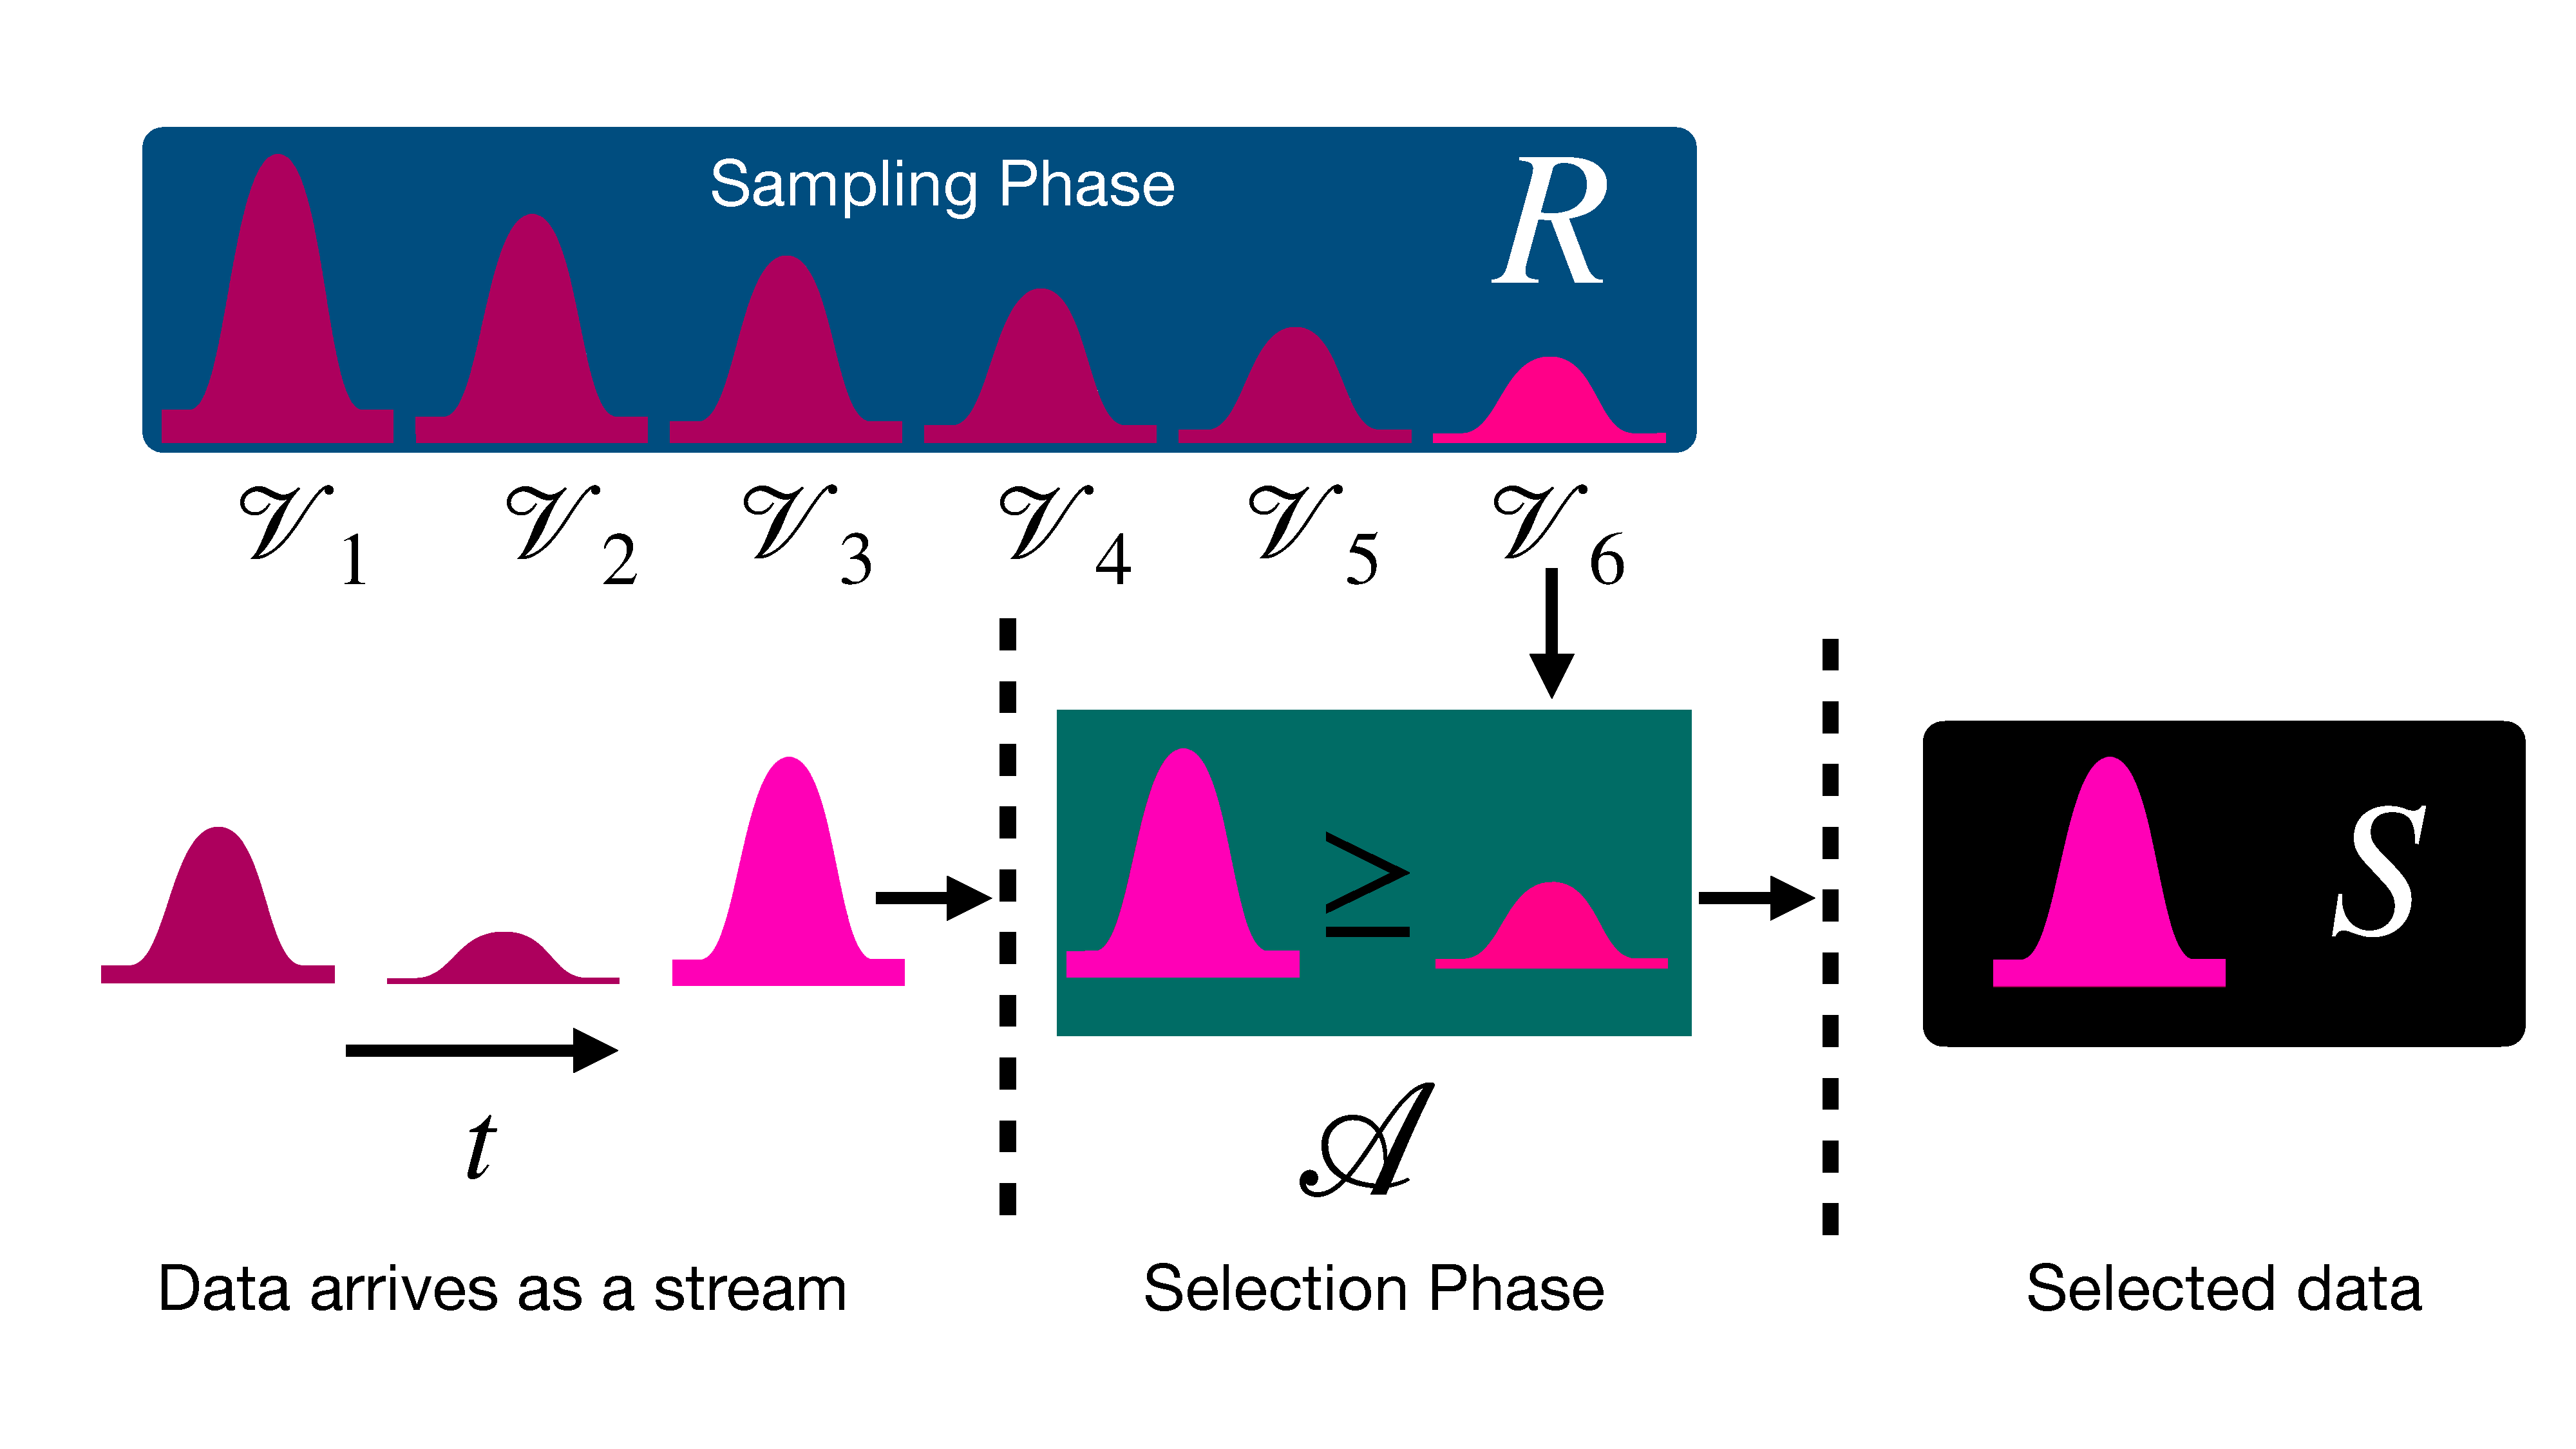
\includegraphics[width=0.48\linewidth]{Figures/stochastic_secretary_fixed.pdf}
    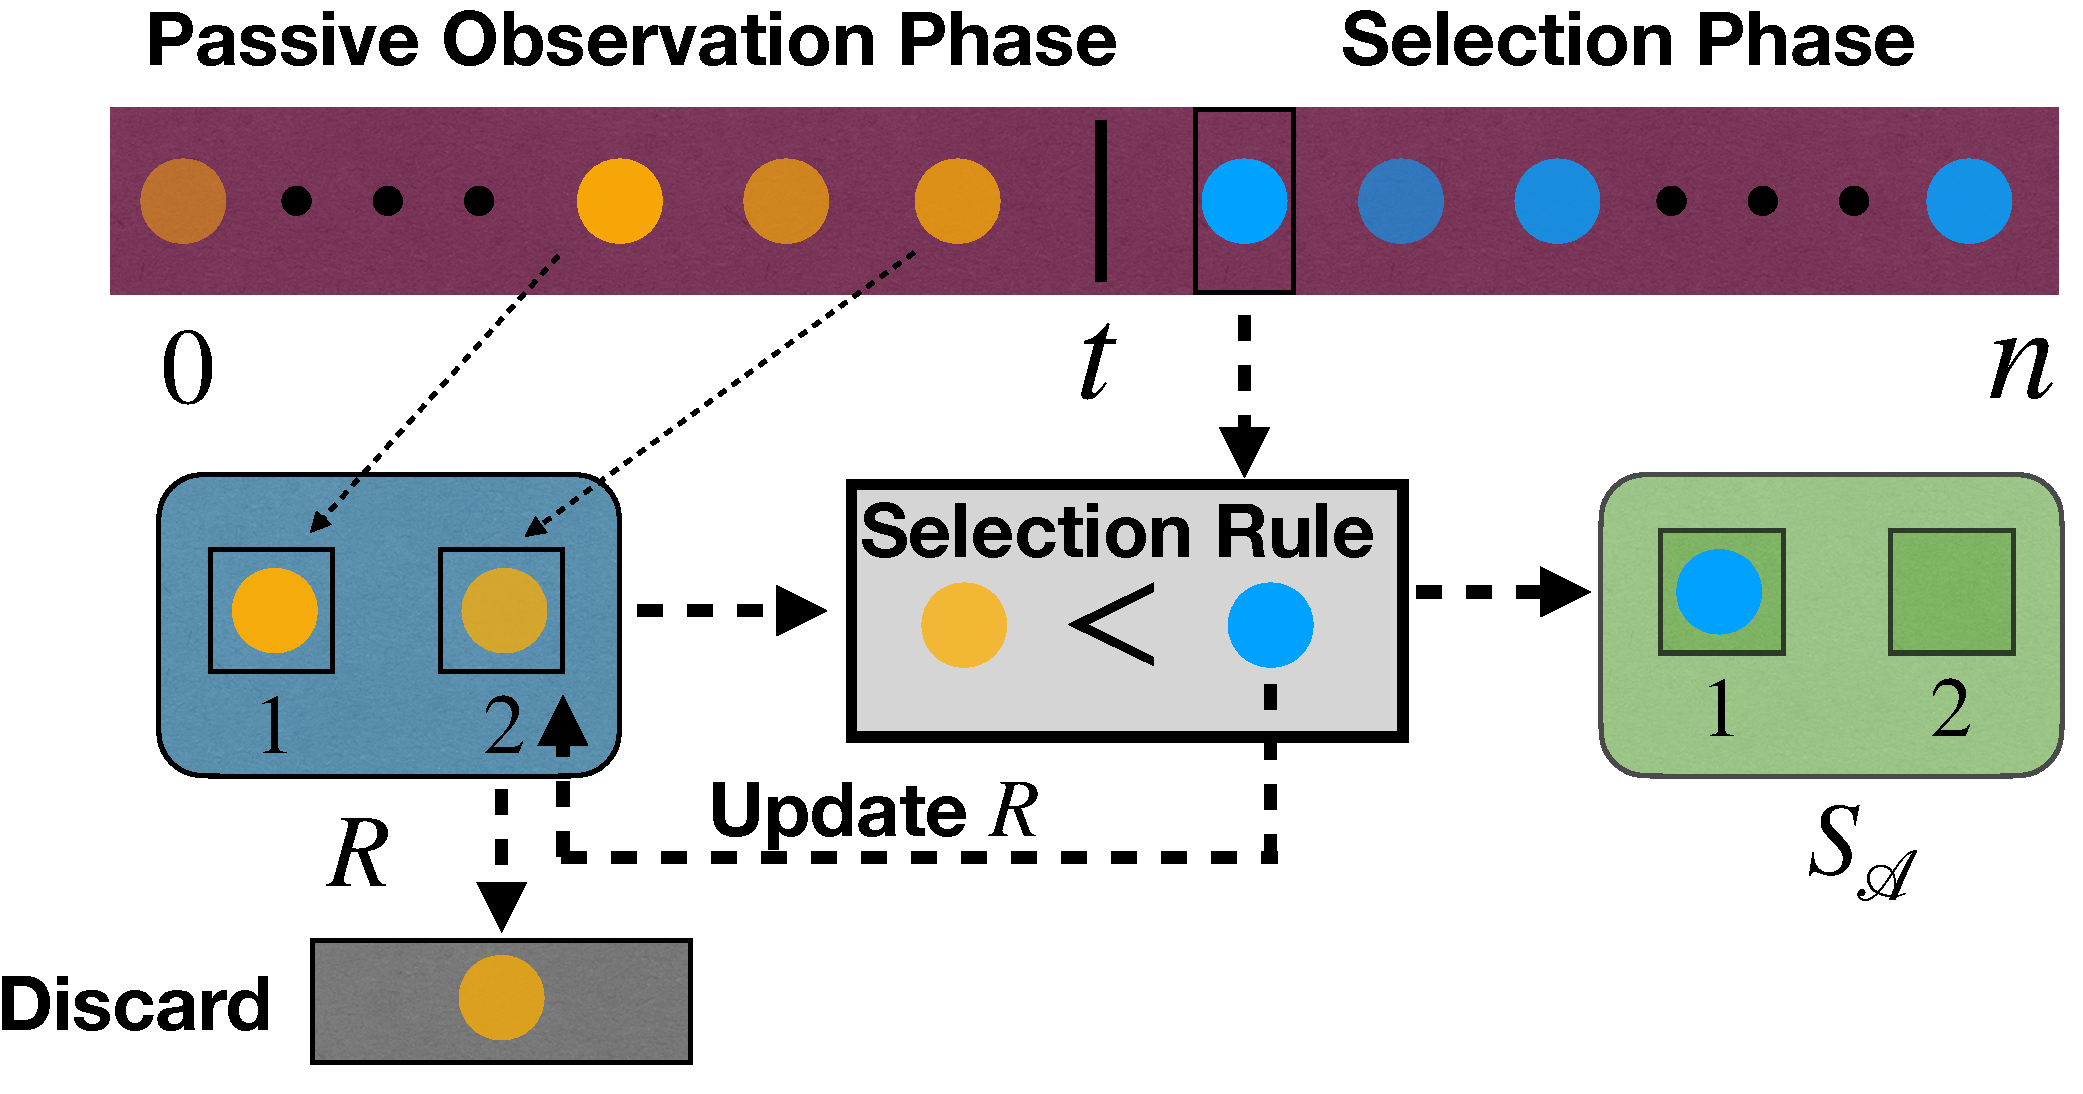
\includegraphics[width=0.48\linewidth]{Figures/Virtual+_algo.pdf}
    %\vspace{-10pt}
    \caption{Each online algorithm, $\mathcal{A}$, observes estimates of $v_i$ and maintains a reference list $R$ during the sampling phase. Items are then picked into $S_{\mathcal{A}}$, after threshold $t$, via comparisons to $R$.}
    \label{fig:stochastic_secretary}
\end{figure}
}
In practice, online adversaries are unlikely to have access to the target model $f_t$.
Instead, it is reasonable to assume that they have partial knowledge. 
%ut instead some partial knowledge. Examples of partial knowledge that have been studied in the blackbox setting include forming input-output queries \cite{ilyas2017query,ilyas2018black,ilyas2018prior} for iterative refinement of an attack vector. However, these sources of knowledge are no longer conducive in the online setting due to transiency of data and we do not consider them. 
Following \cite{papernot2016practical,bose2020adversarial} we focus on modeling that partial knowledge by equipping the adversary with a surrogate model or representative classifier $f_s$. Using $f_s$ as opposed to $f_t$ means that we can compute the value $\mathcal{V}_i:= \ell(f_s(x_i'),y_i)$ of an incoming data point. This value $\mathcal{V}_i$ acts as an estimate of the value of interest $v_i:=\ell(f_t(x_i'),y_i)$. The {\em stochastic $k$-secretary problem} is then to pick, under the noise model induced by using $f_s$, the optimal subset $S_{\mathcal{A}}$ of size $k$ from $\mathcal{D}$. 
Thus, with no further assumptions on $f_s$ it is unclear whether online algorithms, as defined in ~\S\ref{virtual_plus}, are still serviceable under uncertainty.

\xhdr{Sources of randomness}
Our method relies on the idea that we can use the surrogate model $f_s$ to estimate the value of some adversarial examples on the target model $f_t$. We justify here how partial knowledge on $f_t$ could provide us an estimate of $v_i$.
For example, we may know the general architecture and training procedure of $f_t$, but there will be inherent randomness in the optimization (e.g., due to initialization or data sampling), making it impossible to perfectly replicate $f_t$. 
Consequently, we can view the training of a surrogate model $f_s$---using the same general training procedure---as a sample from a common (for $f_s$ and $f_t$) underlying distribution $\mathcal T$. In that context, it seems reasonable to assume that the random variable $\mathcal{V}_i := \ell(f_s(x'_i),y_i)$ is likely to be close to $v_i := \ell(f_t(x'_i),y_i)$. We formalize this assumption on the random variable $\mathcal{V}_i$ in Eq.~\ref{eq:concentration} below.
% Specifically, if all examples $x'_i\,,\, i\ \in [n]$ do not depend on $f_s$ and $f_t$, we have that $\mathcal{V}_i$ and $v_i$ follow the same distribution, i.e., $\ell(f_s(x'_i),y_i) \stackrel{d}{=} \ell(f_t(x'_i),y_i),\,i\in [n]\,.$\footnote{For our theoretical analysis we only require Eq.~\ref{eq:concentration}}
% \begin{equation}
%     \ell(f_s(x'_i,y_i)) \stackrel{d}{=} \ell(f_t(x'_i,y_i)) \,,\quad i=1,\ldots,n\,.
%     \label{eq:same distribution}
% \end{equation}
% Note that one way to have $x'_i$ not depend on $f_s$ and $f_t$ is to use a third independent model $f_{s'}$  of $f_s$ to craft these adversarial examples. 
% Intuitively, it is more compelling to assess the transferability of an adversarial example $x'_i$ on a classifier that is not the one that has been use to craft $x'_i$--- e.g., an adversarial example may perform well on the model used to craft it but poorly transfer to any other classifier.
% \ggi{address the experimental section!!!!}
% For instance the payoff $\sum_{i=0}^N b_i \ell(f(x_i'),y_i)$ of the $k$-secretary problem is independent of $\mathcal{T}$.

% It is the case for a wide range of distributions such as the Gaussian, the exponential 
% we have for small enough $\epsilon$, 
% \begin{equation}
%     \mathbb{P}[|\mathcal{V}_{i}-v_i| \leq \epsilon] 
%     \geq \frac{\epsilon}{2} f(v_i) \geq 1 - e^{-\frac{\epsilon}{2} f(v_i)} \, \notag 
% \end{equation}
% Thus, by some continuiy

\subsection{Stochastic Secretary Algorithms}
\label{stochastic_secretary_algorithms_section}
To ground our study of online adversarial attacks in this challenging setting, we now define the stochastic $k$-secretary problem. In this setting, we assume to have access to the random variables $\mathcal{V}_i$ and that $v_i$ are fixed for $i = 1, \ldots,n$ and the goal is to maximize a notion of stochastic competitive ratio. This notion is similar to the standard competitive ratio defined in~\eqref{eq:comp_ration} with the small difference that in the stochastic case, the algorithm does not have access to the values $v_i$ but to a random variable (R.V.) $\mathcal{V}_i$ that is an estimate of $v_i$. An algorithm is said to be $C$-competitive in the stochastic setting if asymptotically in $n$,
\begin{equation*}
    \mathbb{E}_{\pi \sim \mathcal{S}_n}[\setvaluemath(S_{\mathcal{A}})] \geq ( C + \mathcal{O}(1)) \setvaluemath(S^*) \,.
    \label{eq:sto_comp_ration}
\end{equation*}
Here the expectation is taken over $\mathcal{S}_n$ (uniformly random permutations of the datastream $\mathcal{D}$ of size $n$) and over the randomness of $\mathcal{V}_i\,,\,i=1,\ldots,n$. $S_{\mathcal{A}}$ and $S^*$ are the set of items chosen by the stochastic online and offline algorithms respectively (note that while the online algorithm has access to $\mathcal{V}_i$, the offline algorithm picks the best $v_i$) and \setvalue\ is a set-value function that determines the sum utility of each algorithms selection. Fig.~\ref{fig:stochastic_secretary} illustrates the execution of threshold based online algorithms in the stochastic setting.

% Formally, let $\pi$ be a random ordering on $\mathcal{D}$ and denote $X_{\pi(i)}$ to be the random variable of the approximate adversarial loss on the $i$-th under $\pi$ data point as modelled under the surrogate model.
% We make the following two assumptions throughout the rest of the paper.

% \begin{algorithm}[H]
% \textbf{Parameters:} $t\in(k\dots n-k]$

% \textbf{Sampling phase (up to time $t$):} Reject the first $t -1 $ elements. Construct reference list $R$ with top $k$ elements seen in the sampling phase.

% \textbf{Selection phase (at time $i>t$):}

% \begin{algorithmic}[1]
% \IF {$v(i) \geq v(j_{\mid R \mid})$} 
%         \STATE $R$ = $\{R \setminus \{j_k\}\}$ \hfill\COMMENT{// Update $R$ by taking out $j_{\mid R \mid}$}
%         \STATE $S = \{ S \cup \{i \}\}$ \hfill\COMMENT{// Select element $i$}

% \ENDIF 

% $i\gets i + 1$
% \end{algorithmic}
%  \caption{Optimistic Algorithm}
% \end{algorithm}


% \begin{lemma}
% For all $a \leq k$, the probability that the  algorithm $A$ selects element $i_a^*$ is $\sP[i_a^* \in S] \geq \frac{t}{n} \ln (\frac{n}{t})$. \red{Insert ref here}
% \end{lemma}
% \begin{lemma}
% For all $a,b \leq k$, if we know that $a \leq b$ (meaning $v_a^* \geq v_b^*$) the probability that the  algorithm $A$ selects element $i_a^*$ is $\sP[i_a^* \in S] \geq \sP[i_b^* \in S]$. 
% \end{lemma}
% \begin{proof}
% If algorithm $A$ is Virtual algorithm, notice that the when picking elements Virtual algorithm does not differentiate between elements with indices $i_a, i_b$ where $a,b \leq k$ since the condition for selecting them will at every moment be satisfied by both of them, since the comparison for selecting is made with the $k-th$ top element seen up to that far and for all $a\leq k$, we have $v(i_a) \geq v(j_{\mid R \mid})$. 
% Therefore, when algorithm A is Virtual Algorithm $\sP[i_a^* \in S]^i =\sP[i_b^* \in S]^i$ for all  $i_a, i_b$ where $a,b \leq k$ at each time step $i$.
% \newline

% If Algorithm $A$ is Optimistic Algorithm let's count the number of permutations when $i_a^*$ is accepted by the algorithm versus the number of permutations when $i_b^*$ is accepted at time step $i$. Let's look at the following permutation $\pi$ in which the element $i_b$ is accepted. In order for element $i_b$ to be accepted at the time step $i$ the knapsack was not full and the condition $v(i_b) \geq v(j_{\mid R \mid})$. 
% Now we look at the permutation $\pi^{'}$ such where permutation $\pi$ 
% \end{proof}

\xhdr{Analysis of the algorithms}
In the stochastic setting all online algorithms observe $\mathcal{V}_i$ that is an estimate of the actual value $v_i$ defined as $\mathcal{V}_i = v_i + \eps_i$. That is, we assume that the distribution of $\mathcal{V}_{i}$ has non-vanishing mass around $v_i$. More formally, we assume that there exists $\sigma>0$ s.t., 
    \begin{equation}
        \mathbb{P}[|\mathcal{V}_{i}-v_i| \geq \sqrt{2}\sigma \epsilon] \leq e^{-\epsilon^2} \,,\quad \forall \epsilon >0\,,\,\forall i \in [n].
        \label{eq:concentration}
    \end{equation}
    % $\epsilon$ and is centered around the actual value $\omega_i$. That is $X_i = \omega_i + \epsilon_i$, where $\eps_i \sim$ subG$(\sigma_i^2)$ and $\sigma_i^2$ is the variance.
Such an assumption is quite mild since it holds, for instance, for any sub-Gaussian distribution that admits a continuous and non-vanishing density around $v_i$.\footnote{We considered the same $\sigma$ for all $\mathcal{V}_{i}$ but a tighter bound is possible by considering a different $\sigma_i$ for each random variable.}
The second quantity of interest is the minimal gap between the actual values $v_i$: 
\begin{equation}
    \Delta = \tfrac{1}{2}\min_{1\leq i \neq j \leq  n } \{\mid v_i - v_j \mid \}
\end{equation}
% Let $i_1^*, i_2^* \dots i_k^*$ be the indexes top $k$ true means. Therefore,  the  optimal  offline  solutions  selects  set  $S^*  =\{i_1^*,i_2^*,...i_k^*\}$, while our online algorithm chooses set $S$.
We can now show that the competitive ratio of any online algorithm in the stochastic setting is the same as the deterministic setting up to a multiplicative factor.

\begin{theorem}\label{thm:stochastic_secretary}
Let $\mathcal{A}$ be a $C_n$-competitive secretary algorithm. When having access to independent random variables $\mathcal{V}_{i},\, i\in [n]$ satisfying Eq.~\ref{eq:concentration}, $\mathcal{A}$ has a stochastic competitive ratio of at least:  
\begin{equation}
    C_n \big(1 - e^{\frac{-\Delta^2}{2\sigma^2}}\big)^{n}
\end{equation}
\end{theorem}

The proof of Thm.~\ref{thm:stochastic_secretary} can be found in \S\ref{appendix:proof_thm2}. Such a theoretical result is quite interesting as the stochastic setting initially appears significantly more challenging due to the non-zero probability that the observed ordering of historical values, $\mathcal{V}_i$, not being faithful to the true ordering based on $v_i$. However, Thm.~\ref{thm:stochastic_secretary} explains that any $C_n$-competitive algorithm $\mathcal{A}$ in the deterministic setting is at least as feasible up to a multiplicative factor in the stochastic setting. In fact, in \S\ref{appendix:proof_thm2} we show this multiplicative factor is precisely the probability that the true ordering \cut{based on $v_i$} is preserved under the assumption in Eq.~\ref{eq:concentration}.


% \begin{align*}
%     \sP_i [i_a^* \in S^{(s)}] 
%     &= \sum_{r=1}^{n} \sP_i[i_r^{(s)} \in S^{(s)} \text{ and } i_r^{(s)} = i_a^*]\\
%     &\geq \sum_{r=1}^{r} \sP_i[i_r^{(s)} \in S^{(s)} \text{ and } i_r^{(s)} = i_a^*]\\
%     &\geq \sum_{r=1}^{k} \sP_i[i_r^* \in S]^i  \sP[X_{i_a^*} \textrm{is }(n - r)\textrm{th order statistic}]
% \end{align*}

% \begin{align*}
%     \sP[i_a^* \in S^{(s)}]
%     \geq \sum_{i =t}^{n}\sum_{r=1}^{k} \sP[i_r^* \in S]^i  \sP[X_{i_a^*} \textrm{is}(n - r)\textrm{th order statistic}]
% \end{align*}
% Now by using LEMMA4.2 put reference - we know that:
% \begin{align*}
%     \sP[i_a^* \in S^{(s)}]
%     & \geq \sum_{i =t}^{n}\sum_{r=1}^{k} \sP[i_k^* \in S]^i  \sP[X_{i_a^*} \textrm{is}(n - r) \textrm{th order statistic}]\\
%     & \geq \sum_{i =t}^{n}\sP[i_k^* \in S]^i \sum_{r=1}^{k}   \sP[X_{i_a^*}\textrm{is}(n - r)\textrm{th order statistic}]\\
%     & \geq \frac{t}{n} \ln (\frac{n}{t}) (1 - e^{\frac{-\Delta}{2\sigma^2}})^{(n - k)}
% \end{align*}

% Therefore, 
% \begin{flalign*}
% & E[A^{(s)}] \geq \sum_{a = 1}^{k}\sP[i_a^* \in S^{(s)}] i_a^* \\
% & = \sum_{a = 1}^{k} \frac{t}{n} \ln (\frac{n}{t}) (1 - e^{\frac{-\Delta}{2\sigma^2}})^{(n - k)}i_a^* = \frac{t}{n} \ln (\frac{n}{t})(1-e^{\frac{-\Delta}{2\sigma^2}})^{(n - k)} \sum_{a = 1}^{k}  i_a^*
% \end{flalign*}
% Which implies that competitive ratio of algorithm $A^{(s)}$ is at least $\frac{t}{n} \ln (\frac{n}{t})(1-e^{\frac{-\Delta}{2\sigma^2}})^{n}$.
% \end{proof}

% \subsection{Robustness of Stochastic Virtual Algorithm versus Stochastic Optimistic Algorithm}
% Let's define robustness factor of algorithm $\mathcal{A}$ as: 
% $\phi$($\mathcal{A}$) = $\frac{CR(\mathcal{A}^{(s)})}{CR(\mathcal{A})}$. (CR - competitive ratio of an algorithm indicative one)  
% \begin{lemma}
% Virtual Algorithm is more robust than Optimistic algorithm aka   $\phi$($\mathcal{A}$ - virtual) $\geq$ $\phi$($\mathcal{A}$ - optimistic).
% \end{lemma}
% \begin{proof}

% \xhdr{Robustness of Stochastic Virtual Algorithm}

% Competitive ratio of virtual algorithm is: 
% $\frac{\sum_{a = 1}^{k}\sP[i_a^* \in S] i_a^*}{\sum_{a = 1}^{k} i_a^*}$, 
% while
% competitive ratio of stochastic virtual algorithm is:
% $\frac{\sum_{a = 1}^{k}\sP[i_a^* \in S^{(s)}] i_a^*}{\sum_{a = 1}^{k} i_a^*} = \frac{\sum_{a = 1}^{k}\sP[i_a^* \in S] i_a^*}{\sum_{a = 1}^{k} i_a^*} (1 - e^{\frac{-\Delta}{2\sigma^2}})^{(i -k)}$
% Notice that in order for any top $k$ elements to be picked by stochastic virtual \textbf{at any moment $i$} it only has to retain (i -k)th order (similar as in proof for stochastic virtual algorithm). Therefore, the previously written equality. From two previously written equations we get that the robustness factor of is:
%  $\phi$($\mathcal{A}$ - virtual) = $(1 - e^{\frac{-\Delta}{2\sigma^2}})^{(i -k)}$.
 
% \xhdr{Robustness of Stochastic Optimistic Algorithm}
%  Notice that in order for any top $k$ elements to be picked by stochastic optimistic algorithm \textbf{at any moment $i$} it only has to retain (i -k + f)th order (where $f$ is the number of elements already selected up to moment $i$). Since knapsack will not always be empty and therefore $f$ will not always be zero, following similar derivation as for the Robustness of Stochastic Virtual Algorithm we get that  $\phi(\mathcal{A} - virtual) \geq \phi (\mathcal{A} - optimistic)$. 
% \end{proof}

% \subsection{Correct Global Ordering}
% Let's look at the permutation $\pi$ of indices where:
% $\omega_{\pi(1)}>\omega_{\pi(2)}\dots>\omega_{\pi(n)}$.
% In this example we want to calculate probability that true ordering is preserved aka: 

% \begin{align*}
% &\sP (X_{\pi(1)} > X_{\pi(2)} \dots > X_{\pi(n)}) \\
% & =\sP(X_{\pi(1)}>X_{\pi(2)})
% \prod_{i=2}^{n-1}\sP(X_{\pi(i)}>X_{\pi(i+1)}|\sP(X_{\pi(1)}>\dots X_{\pi(i)})\\
%     &\geq \prod_{i=1}^{n-1}\sP(X_{\pi(i)}>X_{\pi(i+1)}) 
%     = \prod_{i=1}^{n} (1- \sP(X_{\pi(i)} < X_{\pi(i+1)}) \\
%     & \geq (1 - e^{\frac{-\Delta}{2\sigma^2}})^{\frac{n(n-1)}{2}}
% \end{align*}
 
% where $\Delta = \smash{\displaystyle\min_{i, j = 1 \dots n}_{i \neq j}} \{\mid \omega_i - \omega_j \mid \}$.



\subsection{Results on Synthetic Data}
We assess the performance of classical single threshold online algorithms and \algoname\ in solving the stochastic $k$-secretary problem on a synthetic dataset of size $n=100$ with $k \in [1,10]$. The value of a data point is its index in $\mathcal{D}$ prior to applying any permutation $\pi \sim \mathcal{S}_n$ plus noise $\mathcal{N}(0, \sigma^2)$. We compute and plot the competitive ratio over $10k$ unique permutations of each algorithm in Figure \ref{fig:synthetic_data}. 

\begin{minipage}[t]{.48\textwidth}
\begin{figure}[H]
    % \vspace{-5pt}
    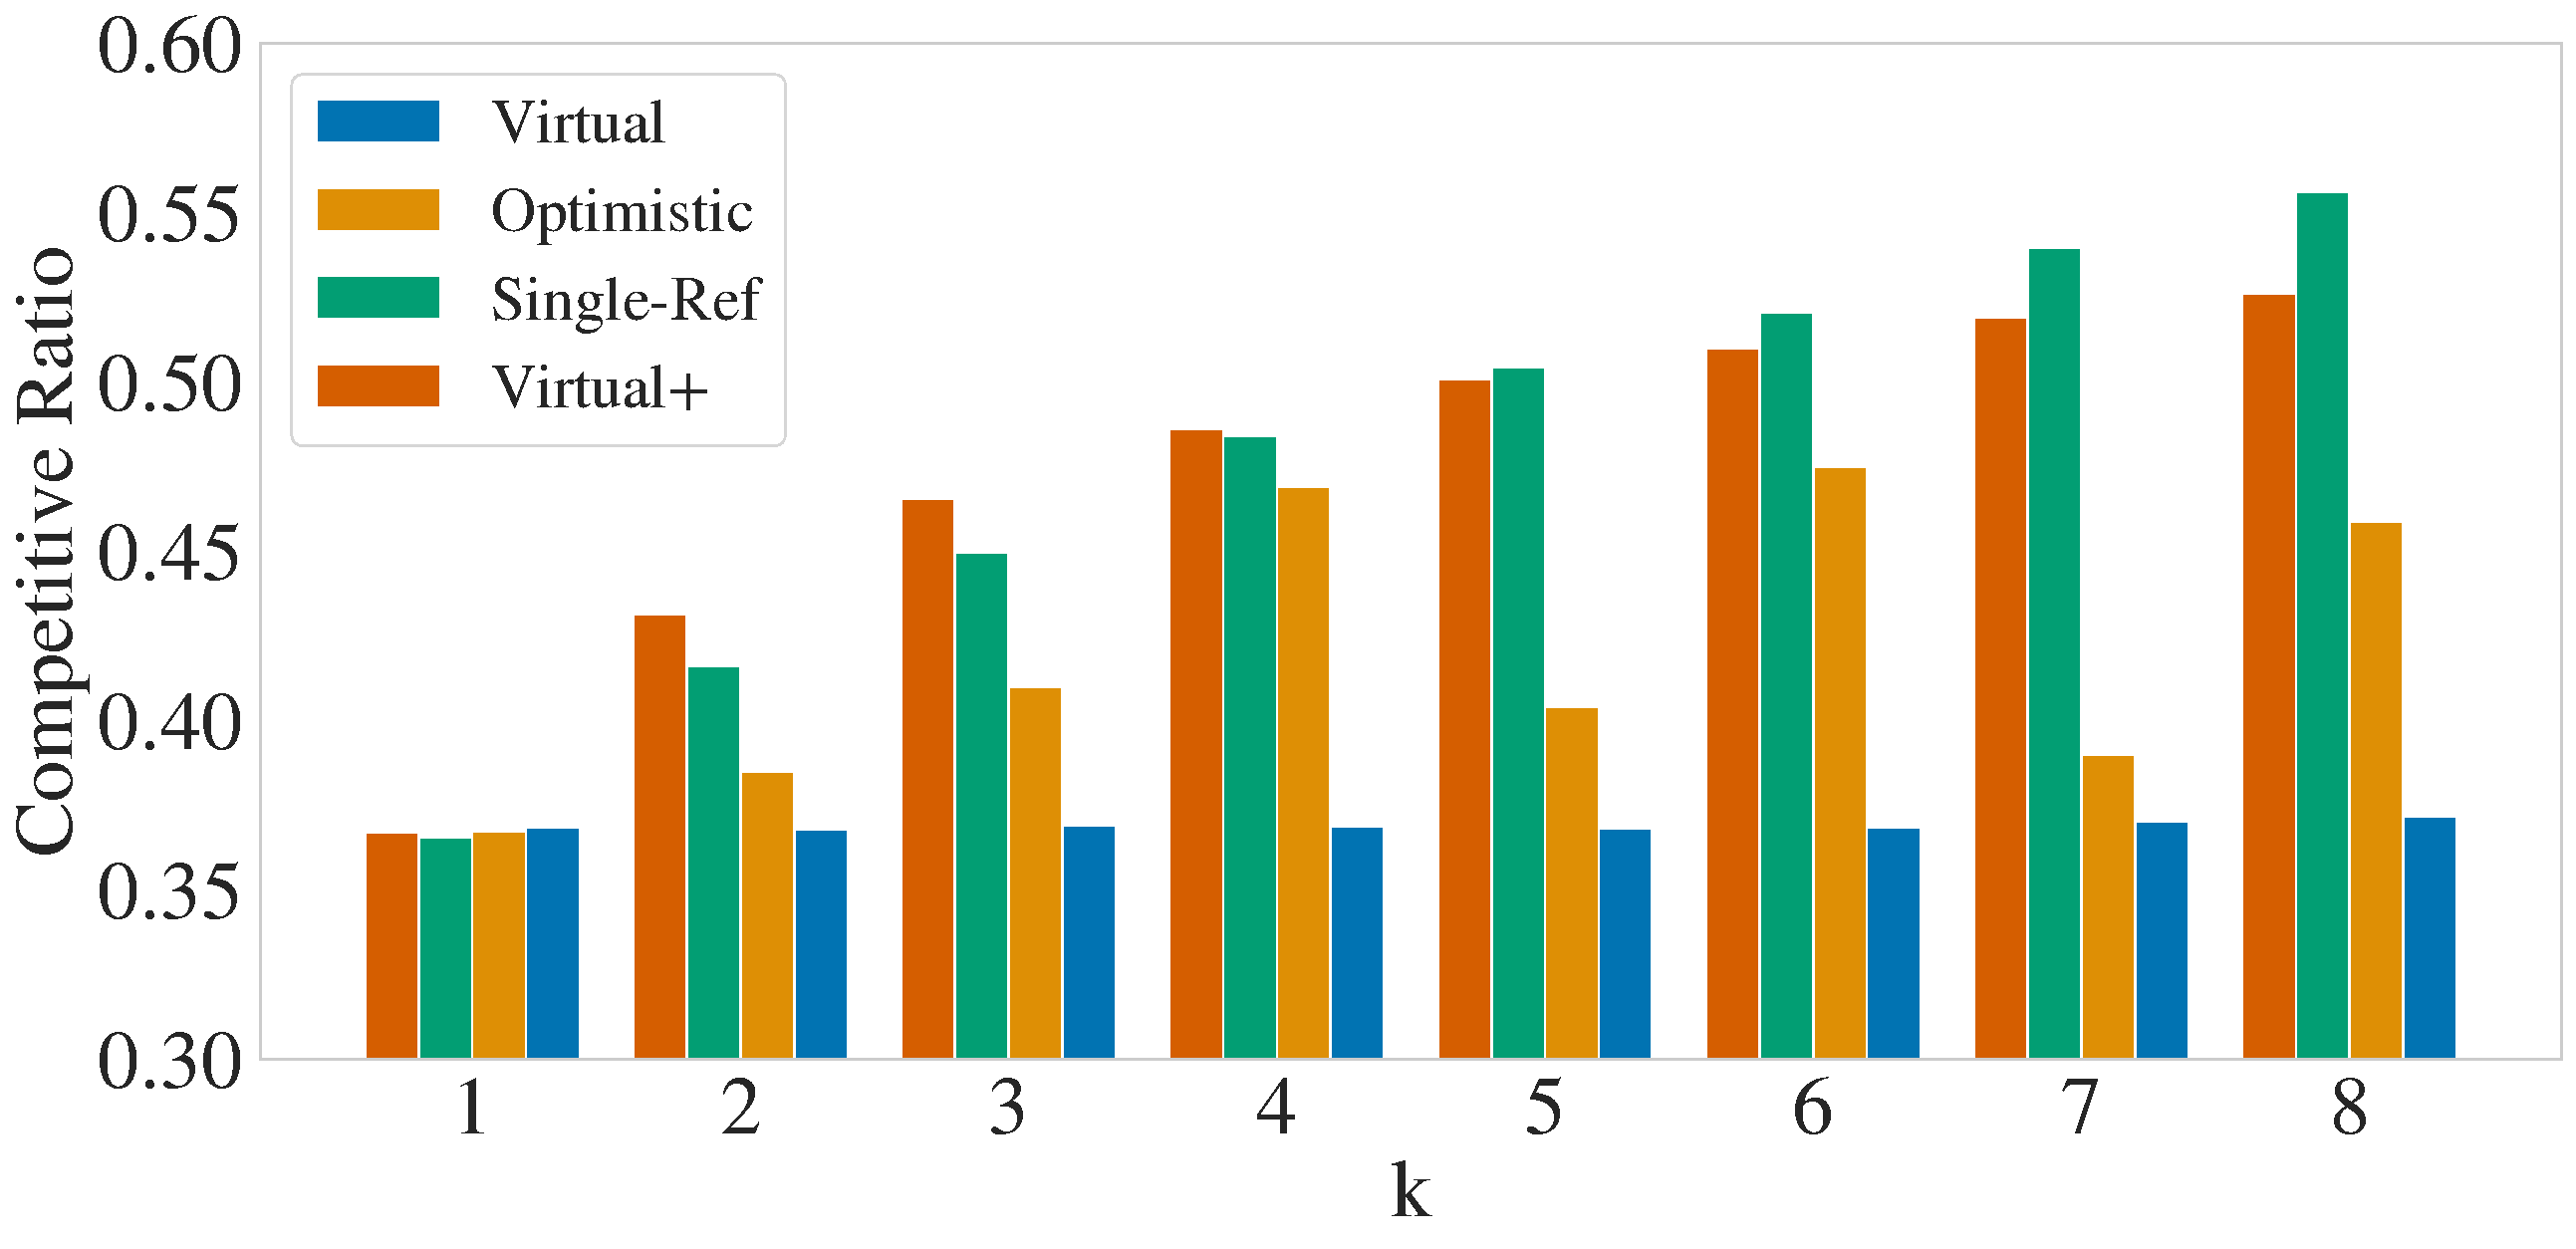
\includegraphics[width=1.01\linewidth]{Figures/Competitive_Ratio3Bar8-Var-10.pdf}
    % \vspace{-15pt}
    \caption{Estimation of the competitive ratio of online algorithms in the stochastic $k$-secretary problem with $\sigma^2=10$.}
    \label{fig:synthetic_data}
\end{figure}
\end{minipage}
\hfill
\begin{minipage}[t]{.48\textwidth}
\vspace{0pt}  
    \begin{algorithm}[H]
    \small
    \textbf{Inputs:} Permuted Datastream: $\mathcal{D}_\pi$, Online Algorithm: $\mathcal{A}$,  Surrogate classifier: $f_s$, Target classifier: $f_t$,  Attack method: \textsc{Att}, Loss: $\ell$,  Budget: $k$,  
    Online Fool rate: $F^{\mathcal{A}}_\pi=0$.
    \begin{algorithmic}[1]
    \FOR{$(x_i,y_i)$ in $\mathcal{D}_\pi$}
    \STATE $x_i' \leftarrow  \textsc{Att}(x_i)$ \hfill \COMMENT{// Compute the attack}
    \STATE $\mathcal{V}_i \leftarrow \ell(f_s(x_i'),y_i)$  \hfill \COMMENT{// Compute the estimate of $v_i$}
    \IF{$\mathcal{A}(\mathcal{V}_1,\ldots, \mathcal{V}_i,k) == \textsc{True}$}
    \STATE  $F^{\mathcal{A}}_\pi \leftarrow F^{\mathcal{A}}_\pi+\tfrac{\mathbf{1}\{f_t(x_i')\neq y_i\}}{k}$  \hfill\COMMENT{// Submit  $x_i'$ on $f_t$} 
    \ENDIF
    \ENDFOR
    \STATE \textbf{return:} $F^{\mathcal{A}}_\pi$ \hfill\COMMENT{//$\mathcal{A}$ always submits $k$ attacks} 
    \end{algorithmic}
     \caption{\small Online Adversarial Attack}
     \label{alg:online_adv_attack}
    \end{algorithm}
\end{minipage}

As illustrated for $k=1$ all algorithms roughly achieve the optimal $(1/e)$-deterministic competitive ratio in the stochastic setting. Note that the noise level, $\sigma^2$, appears to have a small impact on the performance of the algorithms (\S\ref{appendix:synthetic_additional_results}). 
This substantiates our result in Thm.~\ref{thm:stochastic_secretary} indicating that $C_n$-competitive algorithms only degrade by a small factor in the stochastic setting. For $k=2$, \algoname\ achieves the best competitive ratio validating our main result in Thm \ref{thm:K_2_theorem1}. \algoname\ continues to perform favorably for small values $k<5$ after which \textsc{Single-Ref} is superior. 
This was expected as we note that the hyperparameters in \textsc{Single-Ref}---e.g. $t$ and reference rank---are tuned offline for each value of $k$ by solving a separate combinatorial optimization problem while in \algoname\ we use the optimal $t$ for $k=2$ found in Eq.~\ref{eq:alpha_eqn}. We hypothesize that finding optimal thresholds for $k>2$ will further aid the performance of \algoname\ but leave this as future work.
\section{Experiments}
\label{section:experiments}
We investigate the feasibility of online adversarial attacks by considering an online version of the challenging NoBox setting \citep{bose2020adversarial} in which the adversary must generate attacks without any access, including queries, to the target model $f_t$. Instead, the adversary only has access to a surrogate $f_s$ which is similar to $f_t$. In particular, we pick at random a $f_t$ and $f_s$ from an ensemble of pre-trained models from various canonical architectures. We perform experiments on the MNIST \cite{lecun-mnisthandwrittendigit-2010} and CIFAR-10 \cite{krizhevsky2009learning} datasets where we simulate a $\mathcal{D}$ by generating $1000$ permutations of the test set and feeding each instantiation to Alg.~\ref{alg:online_adv_attack}. In practice, online adversaries compute the value 
%$\mathcal{V}_i$ 
$\mathcal{V}_i=\ell(f_s(x'_i),y_i)$ 
of each data point in $\mathcal{D}$ by attacking $f_s$ using their fixed attack strategy
(where $\ell$ is the cross-entropy),
but the decision to submit the attack to $f_t$ is done using an online algorithm~$\mathcal{A}$ (see Alg.~\ref{alg:online_adv_attack}). 
As representative attack strategies, we use the well-known FGSM attack \citep{goodfellow2014explaining} and a universal whitebox attack in PGD \citep{madry2017towards}. 
We are most interested in evaluating the online fool rate, which is simply the ratio of successfully executed attacks against $f_t$ out of a possible of $k$ attacks selected by $\mathcal{A}$. \cut{Attacks are conducted with respect to the $\ell_\infty$- norm with $\gamma = 0.3$ for MNIST and $\gamma = 0.03125$ for CIFAR-10.} The architectures used for $f_s$, $f_t$, and additional metrics (e.g. competitive ratios) can be found in \S\ref{appendix:additional_results}. 

% \setlength{\textfloatsep}{0pt}% Remove \textfloatsep
\cut{
\begin{minipage}[t]{.5\linewidth}
\vspace{0pt}  
    \begin{algorithm}[H]
    \small
    \textbf{Inputs:} Permuted Datastream:$\mathcal{D}_\pi$, \, Online Algorithm:$\mathcal{A}$, \, Surrogate classifier:$f_s$,\, Target classifier:$f_t$,\, Attack method:$\textsc{Att}$,\, Loss:$\ell$, \, Budget:$k$,\, 
    Fool rate: $F^{\mathcal{A}}_\pi=0$.
    \begin{algorithmic}[1]
    \FOR{$(x_i,y_i)$ in $\mathcal{D}_\pi$}
    \STATE $x_i' \leftarrow  \textsc{Att}(x_i)$ \hfill \COMMENT{// Compute the attack}
    \STATE $\mathcal{V}_i \leftarrow \ell(f_s(x_i'),y_i)$  \hfill \COMMENT{// Compute the estimate of $v_i$}
    \IF{$\mathcal{A}(\mathcal{V}_1,\ldots, \mathcal{V}_i,k) == \textsc{True}$}
    \STATE  $F^{\mathcal{A}}_\pi \leftarrow F^{\mathcal{A}}_\pi+\tfrac{\mathbf{1}\{f_t(x_i')\neq y_i\}}{k}$  \hfill\COMMENT{// Submit  $x_i'$ on $f_t$} 
    \ENDIF
    \ENDFOR
    \STATE \textbf{return:} $F^{\mathcal{A}}_\pi$ \hfill\COMMENT{// Note that $\mathcal{A}$ always submits $k$ attacks} 
    \end{algorithmic}
     \caption{\small Online Adversarial Attack}
     \label{alg:online_adv_attack}
    \end{algorithm}
\end{minipage}
}

\xhdr{Baselines} 
To evaluate the utility of picking adversarial examples using online algorithms we rely on two main baselines. First, we use a \textsc{naive} baseline--a lower bound on achievable performance--where the examples to attack are picked uniformly at random, and an upper bound with the \textsc{OPT} baseline where attacks, while crafted using $f_s$, are submitted by using the true value $v_i$ and thus utilizes $f_t$.% These baselines respectively give lower and upper bounds on the performance of an online algorithm. 
% In addition, we also use \textsc{Virtual}, \textsc{Optimistic}, and \textsc{Single-Ref} as baselines for single threshold online algorithms.
\setlength{\textfloatsep}{5pt}% Remove \textfloatsep
\begin{figure*}[t]
    \centering
    %\vspace{-2mm}
    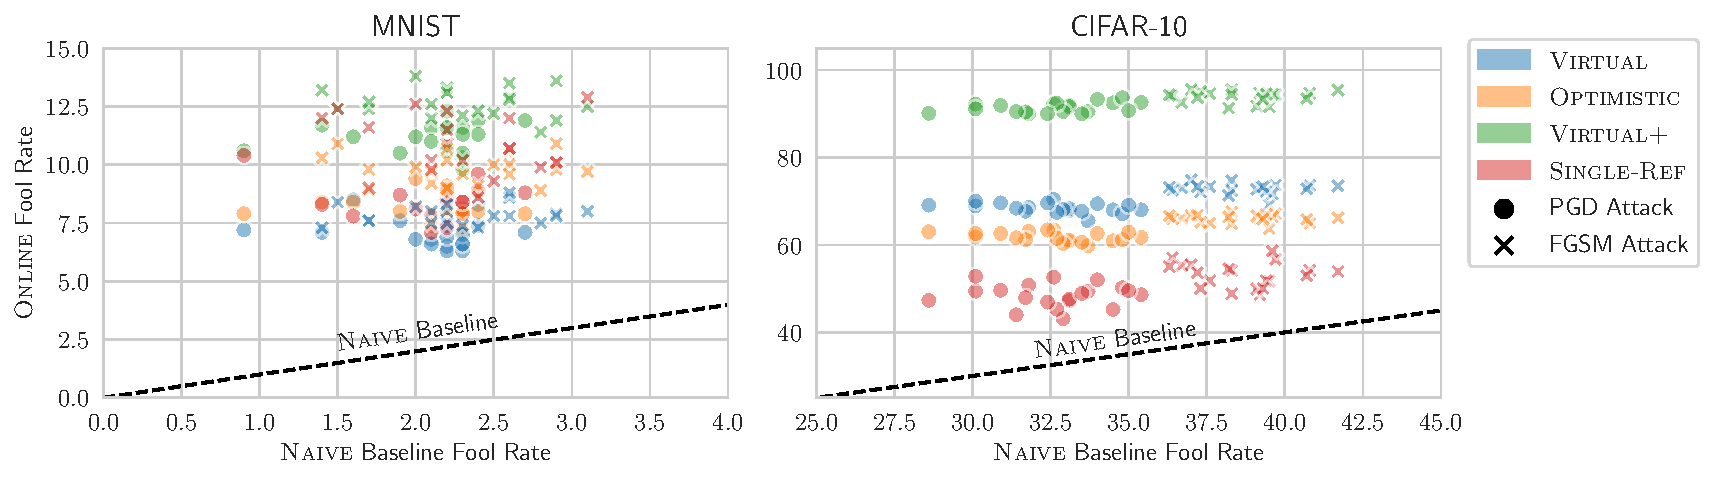
\includegraphics[width=.9\linewidth]{Figures/scatterplot_Q1.pdf}
    %\vspace{-4mm}
    \caption{ \small
    Plot of online fool rates for $k=1000$ against PGD-robust models using different online algorithms $\mathcal{A}$, attacks, datasets, and $20$ different permutations. For a given $x$-coordinate, a higher $y$-coordinate is better.} %The line $y=x$ corresponds to the \textsc{Naive} baseline.}
    \label{fig:scatter}
    %\vspace{-10pt}
\end{figure*}

\xhdr{Q1: Utility of using an online algorithm}
We first investigate the utility of using an online algorithm in selecting data points to attack in comparison to the \textsc{Naive} baseline. For a given permutation $\pi$ and an attack method (FGSM or PGD), we compute the online fool rate of the \textsc{Naive} baseline and online algorithms as $F^{\textsc{Naive}}_\pi$, $F^{\mathcal{A}}_\pi$ respectively. In Fig.~\ref{fig:scatter}, we uniformly sample $20$ permutations $\pi_i \sim \mathcal{S}_n, \, i \in [n],$ of $\mathcal{D}$ and plot a scatter graph of points with coordinates $(F^{\textsc{Naive}}_{\pi_i}, F^{\mathcal{A}}_{\pi_i})$, for different online algorithms $\mathcal{A}$, attacks with $k=1000$,\footnote{\small \url{https://github.com/MadryLab/[x]_challenge}, for $\texttt{[x]} \in \texttt{\{MNIST, CIFAR10 \}}$ .} and datasets. The line $y=x$ corresponds to the \textsc{Naive} baseline performance ---i.e. points with coordinates $(F^{\textsc{Naive}}_\pi, F^{\textsc{Naive}}_\pi)$---and each point above that line corresponds to an online algorithm that outperforms the naive baseline on a specific permutation $\pi_i$. As observed, all online algorithms significantly outperform the \textsc{Naive} baseline, on sampled $\pi_i$'s with an average aggregate improvement of 7.5\% and 34.1\% on MNIST and CIFAR-10.


\begin{table*}[ht]
%\vspace{-10pt}
%\begin{small}
\small
\caption{Online fool rate of various online algorithms on non-robust models. For a given attack and value of $k$: {\color{g1} $\mathbf{\bullet}$ } at least 97\%,
\textbf{\color{g2} $\mathbf{\bullet}$} at least 95\%, \textbf{\color{g3}$\mathbf{\bullet}$} at least 90\%, \textbf{\color{g4} $\mathbf{\bullet}$} less than 90\% of the optimal performance.}% achievable given by \textsc{Opt} in \textbf{bold}.}
\vspace{-5pt}
\label{table:non_robust_table1}
 \begin{center}\begin{tabular}{ c c c c c c c c }
 \toprule
 & & \multicolumn{3}{c}{MNIST (Online fool rate in \%)} & \multicolumn{3}{c}{CIFAR-10  (Online fool rate in \%)}\\
%  \cmidrule{3-8}
 & Algorithm & $k=10$ & $k=100$ & $k=1000$ & $k=10$ & $k=100$ & $k=1000$ \\
 \midrule
 \multirow{6}{*}{\rotatebox[origin=c]{90}{FGSM}}
 %\multirow{6}{*}{FGSM}
 & \textsc{Naive}& 64.1 $\pm$ 33 & 47.8 $\pm$ 31 & 45.7 $\pm$ 31 & 60.7 $\pm$ 17 & 59.2 $\pm$ 6.2 & 59.2 $\pm$ 4.3\\
 & \textsc{Opt}  & \textbf{87.0 $\pm$ 0.5} & \textbf{84.7 $\pm$ 0.5} &  \textbf{83.6 $\pm$ 0.4} & \textbf{86.6 $\pm$ 0.4} & \textbf{87.3 $\pm$ 0.3} &  \textbf{86.5 $\pm$ 0.2} \\
 \cmidrule{2-8}
 %\bottomrule
 %& \textsc{Best Online} & \cellcolor{g1} 76.3 $\pm$ 27.6 & 55.0 $\pm$ 28.8 & 52.9 $\pm$ 26.7\\
 %& \textsc{Worst Online} & \cellcolor{g3} 69.8 $\pm$ 31.9 & 52.6 $\pm$ 29.7 & 49.0 $\pm$ 28.7 \\
 %  \cmidrule{2-8}
 & \textsc{Optimistic} & \cellcolor{g3}79.0 $\pm$ 0.5 & \cellcolor{g3}77.6 $\pm$ 0.4 &\cellcolor{g3} 75.3 $\pm$ 0.4 &\cellcolor{g4} 75.3 $\pm$ 0.5 & \cellcolor{g4} 72.8 $\pm$ 0.2 &\cellcolor{g4} 71.9 $\pm$ 0.2\\
 & \textsc{Virtual} & \cellcolor{g3}78.6 $\pm$ 0.5 &\cellcolor{g3} 79.1 $\pm$ 0.4 &\cellcolor{g3} 77.4 $\pm$ 0.4 & \cellcolor{g4} 76.1 $\pm$ 0.5 &\cellcolor{g4} 77.1 $\pm$ 0.2 & \cellcolor{g4}75.4 $\pm$ 0.2\\
 & \textsc{Single-Ref} &\cellcolor{g2}85.1 $\pm$ 0.5 & \cellcolor{g1}83.0 $\pm$ 0.5 &\cellcolor{g4} 72.3 $\pm$ 0.5 &\cellcolor{g3} 80.4 $\pm$ 0.5 &\cellcolor{g2} 84.0 $\pm$ 0.3 & \cellcolor{g4}66.0 $\pm$ 0.2\\
 & \algoname & \cellcolor{g3}80.4 $\pm$ 0.5 &\cellcolor{g1} 82.5 $\pm$ 0.4 & \cellcolor{g1} 82.9 $\pm$ 0.4 &\cellcolor{g2} 82.9 $\pm$ 0.5 & \cellcolor{g1}86.3 $\pm$ 0.3 &  \cellcolor{g1}85.2 $\pm$ 0.2\\
 \midrule
 %\multirow{6}{*}{PGD}
  \multirow{6}{*}{\rotatebox[origin=c]{90}{PGD}}
 & \textsc{Naive} & 69.7  $\pm$ 16 & 67.2 $\pm$ 20 & 67.9 $\pm$ 18 & 72.5 $\pm$ 18 & 70.4 $\pm$ 9.4 & 68.6 $\pm$ 6.3\\
 & \textsc{Opt} & \textbf{73.6 $\pm$ 0.9} & \textbf{49.8 $\pm$ 0.8} & \textbf{49.6 $\pm$ 0.8} & \textbf{83.7 $\pm$ 0.6} & \textbf{80.6 $\pm$ 0.6} & \textbf{79.9 $\pm$ 0.5}\\
 \cmidrule{2-8}
 %\bottomrule
 & \textsc{Optimistic} & \cellcolor{g3} 66.2 $\pm$ 1.1 & \cellcolor{g2} 48.2 $\pm$ 0.8 &\cellcolor{g3} 45.1 $\pm$ 0.9 &\cellcolor{g3} 79.1 $\pm$ 0.6 & \cellcolor{g3}76.6 $\pm$ 0.4 & \cellcolor{g3}76.0 $\pm$ 0.4\\
 & \textsc{Virtual} &\cellcolor{g4} 63.4 $\pm$ 1.1 & \cellcolor{g4}46.2 $\pm$ 0.9 &\cellcolor{g2} 46.8 $\pm$ 0.8 & \cellcolor{g3}78.3 $\pm$ 0.6 &\cellcolor{g3} 77.5 $\pm$ 0.5 &\cellcolor{g3} 76.9 $\pm$ 0.4\\
 &\textsc{Single-Ref} & \cellcolor{g1} 71.5 $\pm$ 0.9 & \cellcolor{g1} 49.7 $\pm$ 0.8 & \cellcolor{g4}42.9 $\pm$ 0.9 & \cellcolor{g2}80.2 $\pm$ 0.6 &\cellcolor{g1} 79.6 $\pm$ 0.5 & \cellcolor{g4} 74.5 $\pm$ 0.4\\
 & \algoname         &\cellcolor{g2} 68.2 $\pm$ 1.0 & \cellcolor{g1}49.3 $\pm$ 0.8 & \cellcolor{g1} 49.7 $\pm$ 0.8 & \cellcolor{g1} 81.2 $\pm$ 0.6 & \cellcolor{g1} 80.1 $\pm$ 0.6 &\cellcolor{g1}79.5 $\pm$ 0.5\\
 \bottomrule
\end{tabular}\end{center} 
%\end{small}
%\vspace{-15pt}
\end{table*}


\xhdr{Q2: Online Attacks on Non-Robust Classifiers}
\cut{
While previous work on online algorithms focused largely on the theoretical contribution, we are equally interested in their performance in practical applications, where the assumptions of the theory may not necessarily hold anymore.}We now conduct experiments on non-robust MNIST and CIFAR-10 classifiers.\cut{
We thus decide to propose the first comparison of online algorithms in the context of attacking non-robust MNIST and CIFAR-10 classifiers}. We report the average performance of all online algorithms, and the optimal offline algorithm \textsc{Opt} in Tab.~\ref{table:non_robust_table1}. For MNIST, we find that the two best online algorithms are \textsc{Single-Ref} and our proposed \algoname\ which approach the upper bound provided by \textsc{Opt}. For $k=10$ and $k=100$, \textsc{Single-Ref} is slightly superior while $k=1000$ \algoname\ is the best method with an average relative improvement of $15.3\%$. This is unsurprising as \algoname\ does not have any additional hyperparameters unlike \textsc{Single-Ref} which appears more sensitive to the choice of optimal thresholds and reference ranks, both of which are unknown beyond $k=100$ and non-trivial to find in closed form (see \S\ref{appendix:additional_results_larger_datasets} for details). On CIFAR-10, we observe that \algoname\ is the best approach regardless of attack strategy and the online attack budget $k$. A notable observation is that even conventional whitebox adversaries like FGSM and PGD can be turned into strong blackbox transfer attack strategies when carefully choosing datapoints to attack using an appropriate $\mathcal{A}$.%, highlighting the importance of carefully choosing data points to attack in the online setting.  


\begin{table*}[ht]
\small
\caption{Online fool rate of various online algorithms on robust models. For a given attack and value of $k$: {\color{g1} $\mathbf{\bullet}$ } at least 90\%,
\textbf{\color{g2} $\mathbf{\bullet}$} at least 80\%, \textbf{\color{g3}$\mathbf{\bullet}$} at least 70\%, \textbf{\color{g4} $\mathbf{\bullet}$} less than 70\% of the optimal performance.}% achievable given by \textsc{Opt} in \textbf{bold}.}
\vspace{-5pt}
\label{table:madry_challenge}
 \begin{center}\begin{tabular}{ c c c c c c c c}
 \toprule
 & & \multicolumn{3}{c}{MNIST (Online fool rate in \%)} & \multicolumn{3}{c}{CIFAR-10 (Online fool rate in \%)}\\
%   \cmidrule{3-8}
 & Algorithm & $k=10$ & $k=100$ & $k=1000$ & $k=10$ & $k=100$ & $k=1000$ \\
 \midrule 
 %\multirow{6}{*}{FGSM}
 \multirow{6}{*}{\rotatebox[origin=c]{90}{FGSM}}
 & \textsc{Naive} & $2.1 \pm 4.5$ & $2.1 \pm 1.4$ & $2.1 \pm 0.4$ & 31.9 $\pm$ 14.2 & 32.6 $\pm$ 4.7 & 32.5 $\pm$ 1.5\\
 & \textsc{Opt} & \textbf{80.0 $\pm$ 0.0} & \textbf{55.0 $\pm$ 0.0} & \textbf{18.9 $\pm$ 0.0} & \textbf{100.0 $\pm$ 0.0} & \textbf{100.0 $\pm$ 0.0} & \textbf{97.2 $\pm$ 0.0}\\
 \cmidrule{2-8}
 & \textsc{Optimistic} & \cellcolor{g3}$49.7 \pm 0.6$ & \cellcolor{g4}$25.7$ $\pm$ $0.1$ &\cellcolor{g3} $9.7$ $\pm$ $0.0$ & \cellcolor{g2}72.4 $\pm$ 0.5 & \cellcolor{g3}64.6 $\pm$ 0.1 & \cellcolor{g3}61.9 $\pm$ 0.0\\
 & \textsc{Virtual} & \cellcolor{g3}49.8 $\pm$ 0.5 & \cellcolor{g3}27.8 $\pm$ 0.1 &\cellcolor{g4} 8.1 $\pm$ 0.0 & \cellcolor{g2}75.1 $\pm$ 0.5 & \cellcolor{g3}74.3 $\pm$ 0.1 & \cellcolor{g2}68.9 $\pm$ 0.0\\
 & \textsc{Single-Ref} & \cellcolor{g2}62.0 $\pm$ 0.7 & \cellcolor{g2}45.2 $\pm$ 0.2 & \cellcolor{g3}10.2 $\pm$ 0.0 & \cellcolor{g2}84.3 $\pm$ 0.6 & \cellcolor{g1}90.9 $\pm$ 0.3 &\cellcolor{g4} 48.6 $\pm$ 0.1\\
 & \algoname & \cellcolor{g2}68.2 $\pm$ 0.5 & \cellcolor{g2}42.2 $\pm$ 0.1 & \cellcolor{g3}{12.7 $\pm$ 0.0} & \cellcolor{g1}91.5 $\pm$ 0.4 & \cellcolor{g1}96.5 $\pm$ 0.1 & \cellcolor{g1}{91.7 $\pm$ 0.0}\\
 \midrule
 %\multirow{6}{*}{PGD}
 \multirow{6}{*}{\rotatebox[origin=c]{90}{PGD}}
 & \textsc{Naive} & 1.8 $\pm$ 4.1 & 1.9 $\pm$ 1.4 & 1.9 $\pm$ 0.4 & 39.1 $\pm$ 14.2 & 38.9 $\pm$ 4.4 & 38.7 $\pm$ 1.5\\
 & \textsc{Opt} & \textbf{58.9 $\pm$ 0.4} & \textbf{39.9 $\pm$ 0.1} & \textbf{16.1 $\pm$ 0.0 }& \textbf{100.0 $\pm$ 0.0} & \textbf{100.0 $\pm$ 0.0} & \textbf{98.0 $\pm$ 0.0}\\
 \cmidrule{2-8}
 & \textsc{Optimistic} & \cellcolor{g2}34.9 $\pm$ 0.5 & \cellcolor{g4}19.2 $\pm$ 0.1 &\cellcolor{g3} 8.2 $\pm$ 0.0 & \cellcolor{g2}75.4 $\pm$ 1.9 & \cellcolor{g3}68.5 $\pm$ 0.4 & \cellcolor{g3}66.0 $\pm$ 0.1\\
 & \textsc{Virtual} & \cellcolor{g2}35.4 $\pm$ 0.5 & \cellcolor{g3}21.8 $\pm$ 0.1 &\cellcolor{g4} 7.2 $\pm$ 0.0 & \cellcolor{g2}78.1 $\pm$ 1.7 &\cellcolor{g2} 77.3 $\pm$ 0.5 & \cellcolor{g2}72.8 $\pm$ 0.1\\
 & \textsc{Single-Ref} &\cellcolor{g1} 44.1 $\pm$ 0.6 & \cellcolor{g2}33.9 $\pm$ 0.2 & \cellcolor{g3}8.3 $\pm$ 0.0 & \cellcolor{g2}86.2 $\pm$ 2.2 &\cellcolor{g1} 91.9 $\pm$ 0.9 & \cellcolor{g3}53.2 $\pm$ 0.3\\
 & \algoname & \cellcolor{g1}48.3 $\pm$ 0.5 & \cellcolor{g2}32.8 $\pm$ 0.1 & \cellcolor{g3}11.1 $\pm$ 0.0 & \cellcolor{g1}92.2 $\pm$ 1.3 & \cellcolor{g1}97.1 $\pm$ 0.4 &\cellcolor{g1} 94.2 $\pm$ 0.1\\
 \bottomrule
\end{tabular}\end{center} 
%\vspace{-15pt}
\end{table*}


\xhdr{Q3: Online Attacks on Robust Classifiers}
We now test the feasibility of online attacks against classifiers robustified using adversarial training. To do so, we adapt the public Madry Challenge \citep{madry2017towards} to the online setting, by attacking a subset of the test set as it is streamed. We report the average performance of each online algorithm in Table ~\ref{table:madry_challenge}. We observe that \algoname\ is the best online algorithms, outperforming \textsc{Virtual} and \textsc{Optimistic}, in all settings except for $k=10$ on MNIST where \textsc{Single-Ref} is slightly better. 
%An interesting observation for CIFAR-10 is that attacks on robust models in comparison to non-robust models lead to higher success rates in the online setting. We reconcile this counter-intuitive fact by noting that even when $k=1000$, it corresponds to only $10\%$ of the test set while a PGD-attack can transfer with 38.7\%  efficacy on the robust model for the entire test set. Thus, the efficiency of an online attacks requires the ability to detect the optimal examples to attack than the global robustness of a model which is highly influenced by the distribution of $\mathcal{V}_i$. For instance, if the value of the examples that correspond to a successful attack cannot be distinguished from the ones that are unsuccessful, then one cannot hope to use an online algorithm---that only observe values---to always manage to pick successful attacks.
% for non-robust models, there may be many equally attackable, but potentially low-value datapoints ---i.e. the distribution of $\mathcal{V}_i$'s is flat. 
% Thus attacking these points might not result in transferable attack vectors against $f_t$. 
% On the other hand, for robust models, there are fewer attackable points and attacking via selections of an online algorithm lead to higher transfer rates on $f_t$. 
%We empirically verify that these distributions of values $\mathcal{V}_i$ for CIFAR-10 robust and non-robust models are relatively different in \S\ref{appendix:visualization_of_values_observed}.

\xhdr{Q4: Differences between the online and offline setting} The online threat model presents several interesting phenomenon that we now highlight. First we observe that a stronger attack (e.g. PGD)---in comparison to weaker ones like FGSM---in the offline setting doesn't necessarily translate to an equivalently stronger attack in the online setting. We explain this phenomenon in Fig.~\ref{fig:fgsm_vs_pgd_loss} \&~\ref{fig:fgsm_vs_pgd_ratio} by plotting the distribution of the loss values and the ratio of unsuccessful attacks to total attacks for PGD and FGSM. We observe that the PGD curve is above the FGSM curve indicating that while PGD is a stronger attacker than FGSM, it is harder for $\mathcal{A}$ to pick successful attacks using PGD. A similar initially counter-intuitive observation can be made when comparing the online fool rate on robust and non-robust classifiers. While it is natural to expect the online fool rate to be lower on robust model we empirically observe the opposite in Tab.~\ref{table:non_robust_table1} and~\ref{table:madry_challenge}. To understand this phenomena we plot the distribution of the ratio of unsuccessful attacks as a function $f_s$'s loss in Fig.~\ref{fig:histogram_Vi}. We observe that non-robust models have a distribution with a heavier tail making it harder for $\mathcal{A}$ to pick successful attacks purely based on loss (see~\S\ref{appendix:visualization_of_values_observed} for more details). 
\begin{figure}[h]
\vspace{-15pt}
    \centering
    \captionsetup[subfigure]{justification=centering}
    \begin{subfigure}[b]{0.32\columnwidth}
    \centering
    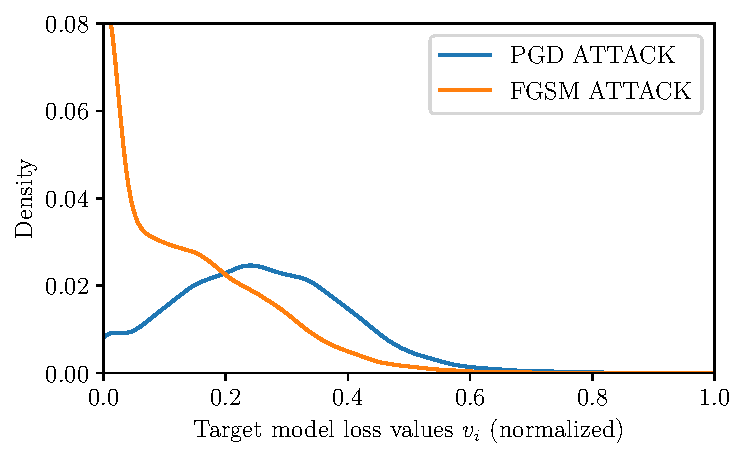
\includegraphics[width=\textwidth]{Figures/fgsm_vs_pgd_loss.pdf}
    \caption{\small Distribution of $f_t$'s loss values for PGD and FGSM}
    \label{fig:fgsm_vs_pgd_loss}
    \end{subfigure}
    \hfill
    \begin{subfigure}[b]{0.32\columnwidth}
    \centering
    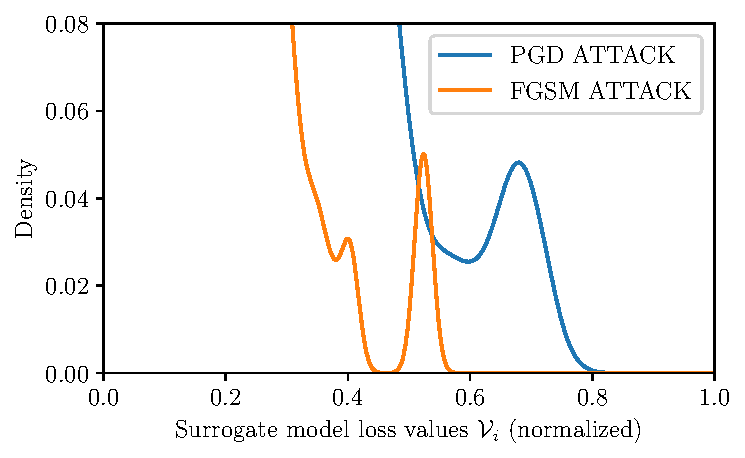
\includegraphics[width=\textwidth]{Figures/fgsm_vs_pgd_ratio.pdf}
    \caption{\small Distribution of the ratio of unsuccessful attacks}
    \label{fig:fgsm_vs_pgd_ratio}
    \end{subfigure}
    \hfill
    \begin{subfigure}[b]{0.32\columnwidth}
    \centering
    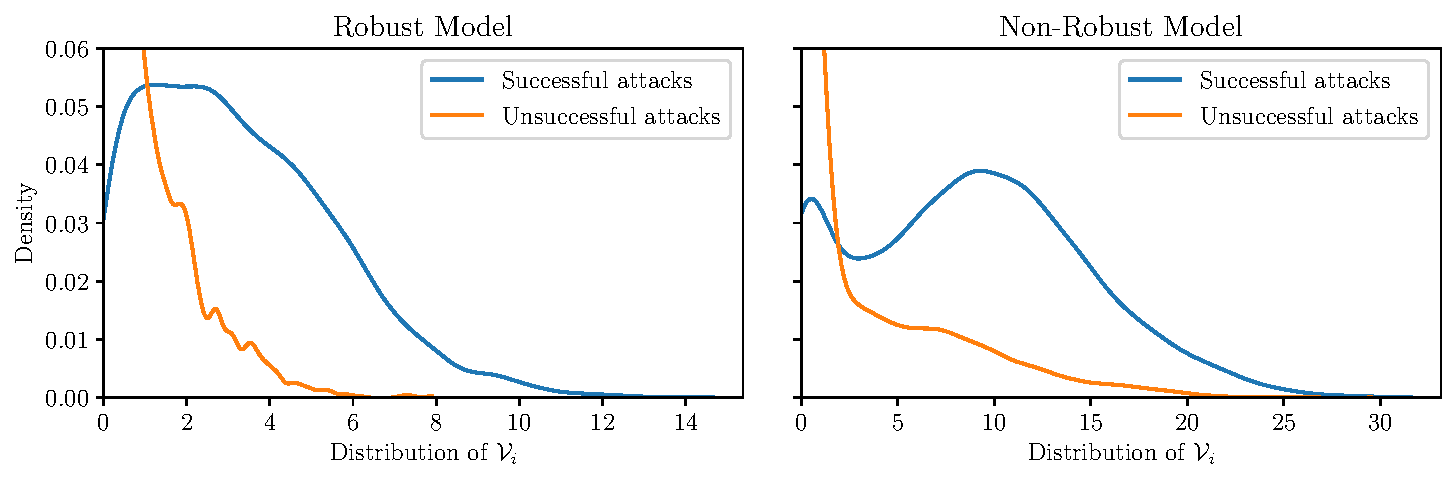
\includegraphics[width=\textwidth]{Figures/histogram_Vi.pdf}
    \caption{\small Distribution of the ratio of unsuccessful attacks}
    \label{fig:histogram_Vi}
    \end{subfigure}
    \caption{\small For every example in MNIST (or CIFAR) we compute an attack using $f_s$ and submit it to $f_t$. \textbf{Left}: The distribution of the normalized loss values of $f_t$ for all attacks where a higher loss is a stronger attack. \textbf{Middle}: The percentage of unsuccessful attacks as a function of $f_s$ normalized loss values. \textbf{Right}: The distribution of the ratio of unsuccessful attacks to total attacks as a function of the $f_s$ normalized loss values.}
    \label{fig:fgsm_vs_pgd}
\end{figure}
\vspace{-20pt}
\section{Related Work}
%Adversarial attacks against deep neural networks were first introduced in \citep{szegedy2013intriguing,goodfellow2014explaining} and since then the field has experienced an explosion of interest in both whitebox settings \cite{madry2017towards,moosavi2016deepfool,carlini2017towards} and more realistic blackbox settings \cite{chen2017zoo,ilyas2018black, jiang2019black,bose2020adversarial, bhambri2019survey,chakraborty2018adversarial}. 
\xhdr{Adversarial attacks} The idea of attacking deep neural networks was first introduced in \citep{szegedy2013intriguing,goodfellow2014explaining}, and recent years have witnessed the introduction of challenging threat models, such as blackbox attacks \cite{chen2017zoo,ilyas2018black, jiang2019black,bose2020adversarial,chakraborty2018adversarial} as well as defense strategies \cite{madry2017towards,tramer2017ensemble,Ding2020MMA}.
Closest to our setting are adversarial attacks against real-time systems \cite{gong2019real, gong2019remasc} and more broadly against deep reinforcement learning agents \cite{lin2017tactics,sun2020stealthy}. However, unlike our work, these approaches are not online algorithms and do not impose constraints of transiency and online attack budgets. 
%Finally, prevalent defence strategies against adversarial attacks include forms of adversarial training which can be interpreted as training classifiers via robust optimization \cite{madry2017towards,tramer2017ensemble,Ding2020MMA}.

\xhdr{$k$-secretary} The classical secretary problem was originally proposed by \cite{gardner1960mathematical} and later solved in \cite{dynkin1963optimum} with an $(1/e)$-optimal algorithm. \citet{kleinberg2005multiple} introduced the $k$-secretary problem and an asymptotically optimal algorithm which achieves a competitive ratio of $1 - \Theta(\sqrt{1/k})$. 
%In the small $k$-regime, \citep{babaioff2007knapsack} proposed both the \textsc{Virtual} and \textsc{Optimistic} algorithms which are $(1/e)$-competitive.\textsc{Single-Ref} \cite{albers2019improved} further improves upon this result by introducing a new hyperparameter called the reference rank and a tuned threshold. 
As outlined in \S\ref{connection_to_prior_work} for $k = 2$ an optimal algorithm exists \cite{chan2014revealing}, but requires the analysis of involved LPs that grow with the size of $\mathcal{D}$. A parallel line of work dubbed the prophet secretary problem, considers online problems where---unlike \S\ref{stochastic_secretary_algorithms_section}---some information on the distribution of values is known \textit{a priori}~\cite{azar2014prophet, azar2018prophet, esfandiari2017prophet}. Secretary problems have also been applied to machine learning, via machine-learned advice which informs the online algorithm about the inputs before execution \cite{antoniadis2020secretary,dutting2020secretaries}. 
Finally, other interesting secretary settings, in addition to the random order model, include playing with adversaries \cite{bradac2019robust, kaplan2020competitive}.




% Prophet Papers:
% -Yossi Azar, Ashish Chiplunkar, and Haim Kaplan.
% Prophet secretary: Surpassing the 1 − 1/e barrier. In Proceedings of the 2018 ACM Conference
% on Economics and Computation (EC), pages 303–co
% 318, 2018.

% -José R. Correa, Raimundo Saona, and Bruno Ziliotto.
% Prophet secretary through blind strategies. In Proceedings of the 30th Annual ACM-SIAM Symposium
% on Discrete Algorithms (SODA), pages 1946–1961,
% 2019.

% -Soheil Ehsani, MohammadTaghi Hajiaghayi, Thomas
% Kesselheim, and Sahil Singla. Prophet secretary for
% combinatorial auctions and matroids. In Proceedings of the 29th Annual ACM-SIAM Symposium on
% Discrete Algorithms (SODA), pages 700–714, 2018.

% -Hossein Esfandiari, MohammadTaghi Hajiaghayi,
% Vahid Liaghat, and Morteza Monemizadeh. Prophet
% secretary. SIAM Journal on Discrete Mathematics,
% 31(3):1685–1701, 2017.


% - Prophet inequalities for i.i.d.
% random variables from an unknown distribution. In Proceedings of the 2019 ACM Conference on
% Economics and Computation, page 3–17, 2019.


% -Paul D¨utting and Thomas Kesselheim. Posted pricing and prophet inequalities with inaccurate
% priors. In Proceedings of the 2019 ACM Conference on Economics and Computation, pages 111–
% 129, 2019.

%Maybe papers - doube check them 
%Moshe Babaioff, Michael Dinitz, Anupam Gupta, Nicole Immorlica, and Kunal Talwar. Secretary problems: weights and discounts. 
%A simple o (log log (rank))-competitive algorithm for the matroid secretary problem
%%Moshe Babaioff, Nicole Immorlica, David Kempe, and Robert Kleinberg. Matroid secretary problems.
%Strong algorithms for the ordinal matroid secretary problem
%Matroid prophet inequalities and applications to multi-dimensional mechanism design
%Optimal single-choice prophet inequalities from samples.
%Strong Algorithms for the Ordinal Matroid Secretary Problem∗
%Prophet Inequalities for Independent Random Variables from an Unknown Distribution
%Recent developments in prophet inequalities
%Prophets, secretaries, and maximizing the probability of choosing the best
%Competitive analysis with a sample and the secretary problem
%The secretary problem with independent sampling
%Prophet secretary for combinatorial auctions and matroids


\section{Conclusion}
In this paper, we formulate the online adversarial attack problem, a novel threat model to study adversarial attacks on streaming data. We propose \algoname, a simple yet practical online algorithm that enables attackers to select easy to fool data points while being theoretically the best single threshold algorithm for $k=2$. We further introduce the stochastic $k$-secretary problem and prove fundamental results on the competitive ratio of any online algorithm operating in this new setting. Our work sheds light on the tight coupling between optimally selecting data points using an online algorithm and the final attack success rate, enabling weak adversaries to perform on par with stronger ones at no additional cost. Investigating, the optimal threshold values for larger values of $k$ along with competitive analysis for the general setting is a natural direction for future work.  

\section*{Societal Impact}
\label{broader_impact}
We introduce the online threat model which aims to capture a new domain for adversarial attack research against streaming data. Such a threat model exposes several new security and privacy risks. For example, using online algorithms, adversaries may now tailor their attack strategy to attacking a small subset of streamed data but still cause significant damage to downstream models e.g. the control system of an autonomous car. On the other hand our research also highlights the need and importance of stateful defence strategies that are capable of mitigating such online attacks. On the theoretical side the development and analysis of \algoname \ has many potential applications outside of adversarial attacks broadly categorized as resource allocation problems. As a concrete example one can consider advertising auctions which provide the main source of monetization for a variety of internet services including search engines, blogs, and social networking sites. Such a scenario is amenable to being modelled as a secretary problem as an advertiser may be able to estimate accurately the bid required to win a particular auction, but may not be privy to the trade off for future auctions.


%\section*{Acknowledgements}

The authors would like to acknowledge Reyhane Askari Hemmat, Tiago Salvador and Noah Marshall for reviewing early drafts of this work.

\textbf{Funding.} This work is partially supported by the Canada CIFAR AI Chair Program (held at Mila).
Joey Bose was also supported by an IVADO PhD fellowship.
Simon Lacoste-Julien and Pascal Vincent are CIFAR Associate Fellows in the Learning in Machines \& Brains program. Finally, we thank Facebook for access to computational resources.
%\section*{Contributions}

% AM and GG formulated the online adverserial attacks setting by drawing parallels to the $k$-secretary problem, with AM leading the theoretical investigation and theoretical results. Joey Bose conceived the idea of online attacks, drove the writing of the paper and helped AM with toy results. Hugo Berard was the chief architect behind all experimental results on MNIST and CIFAR-10.  WH, SLJ and PV provided feedback and guidance over this research while GG supervised the core technical execution of the theory.


\emph{Andjela Mladenovic} and \emph{Gauthier Gidel} formulated the online adverserial attacks setting by drawing parallels to the $k$-secretary problem, with \emph{Andjela Mladenovic} leading the theoretical investigation and theoretical results. \emph{Avishek Joey Bose} conceived the idea of online attacks, drove the writing of the paper and helped \emph{Andjela Mladenovic} with experimental results on synthetic data. \emph{Hugo Berard} was the chief architect behind all experimental results on MNIST and CIFAR-10.  \emph{William L. Hamilton}, \emph{Simon Lacoste-Julien} and \emph{Pascal Vincent} provided feedback and guidance over this research while \emph{Gauthier Gidel} supervised the core technical execution of the theory.

\clearpage
\bibliography{bibliography}
\bibliographystyle{abbrvnat}
%\bibliographystyle{plain}

%%%%%%%%%%%%%%%%%%%%%%%%%%%%%%%%%%%%%%%%%%%%%%%%%%%%%%%%%%%%
\section*{Checklist}
\cut{
%%% BEGIN INSTRUCTIONS %%%
The checklist follows the references.  Please
read the checklist guidelines carefully for information on how to answer these
questions.  For each question, change the default \answerTODO{} to \answerYes{},
\answerNo{}, or \answerNA{}.  You are strongly encouraged to include a {\bf
justification to your answer}, either by referencing the appropriate section of
your paper or providing a brief inline description.  For example:
\begin{itemize}
  \item Did you include the license to the code and datasets? \answerYes{See Section~\ref{gen_inst}.}
  \item Did you include the license to the code and datasets? \answerNo{The code and the data are proprietary.}
  \item Did you include the license to the code and datasets? \answerNA{}
\end{itemize}
Please do not modify the questions and only use the provided macros for your
answers.  Note that the Checklist section does not count towards the page
limit.  In your paper, please delete this instructions block and only keep the
Checklist section heading above along with the questions/answers below.
%%% END INSTRUCTIONS %%%
}
\begin{enumerate}

\item For all authors...
\begin{enumerate}
  \item Do the main claims made in the abstract and introduction accurately reflect the paper's contributions and scope?
    \answerYes{See Sections~\ref{virtual_plus} and~\ref{stochastic_k_secretary} for our main theoretical results.}
  \item Did you describe the limitations of your work?
    \answerYes{Section~\ref{connection_to_prior_work} discusses prior work and~\ref{online_adversarial_attacks} and~\ref{results_on_synthetic_data} show that \algoname\ is optimal up to $k<5$.}
  \item Did you discuss any potential negative societal impacts of your work?
    \answerYes{See section~\ref{broader_impact} for examples of broader impact arising from both the Online Threat Model as well as \algoname.}
  \item Have you read the ethics review guidelines and ensured that your paper conforms to them?
    \answerYes{}
\end{enumerate}

\item If you are including theoretical results...
\begin{enumerate}
  \item Did you state the full set of assumptions of all theoretical results?
    \answerYes{See~\ref{stochastic_secretary_algorithms_section} for key assumptions in the stochastic $k$-secretary setting.}
	\item Did you include complete proofs of all theoretical results?
    \answerYes{See appendices~\ref{appendix:virtual_plus_proof_k_2}, ~\ref{app:general_k_proof}, and~\ref{appendix:proof_thm2} for full proofs of all theoretical results.}
\end{enumerate}

\item If you ran experiments...
\begin{enumerate}
  \item Did you include the code, data, and instructions needed to reproduce the main experimental results (either in the supplemental material or as a URL)?
    \answerYes{}
  \item Did you specify all the training details (e.g., data splits, hyperparameters, how they were chosen)?
    \answerYes{}
	\item Did you report error bars (e.g., with respect to the random seed after running experiments multiple times)?
    \answerYes{}
	\item Did you include the total amount of compute and the type of resources used (e.g., type of GPUs, internal cluster, or cloud provider)?
    \answerNo{}
\end{enumerate}

\item If you are using existing assets (e.g., code, data, models) or curating/releasing new assets...
\begin{enumerate}
  \item If your work uses existing assets, did you cite the creators?
    \answerYes{}
  \item Did you mention the license of the assets?
    \answerNo{}
  \item Did you include any new assets either in the supplemental material or as a URL?
    \answerNo{}
  \item Did you discuss whether and how consent was obtained from people whose data you're using/curating?
    \answerNA{}{}
  \item Did you discuss whether the data you are using/curating contains personally identifiable information or offensive content?
    \answerNA{}
\end{enumerate}

\item If you used crowdsourcing or conducted research with human subjects...
\begin{enumerate}
  \item Did you include the full text of instructions given to participants and screenshots, if applicable?
    \answerNA{Our experiments did not involve the participation of human subjects}
  \item Did you describe any potential participant risks, with links to Institutional Review Board (IRB) approvals, if applicable?
    \answerNA{}
  \item Did you include the estimated hourly wage paid to participants and the total amount spent on participant compensation?
    \answerNA{Our experiments did not involve the participation of human subjects}
\end{enumerate}

\end{enumerate}

%%%%%%%%%%%%%%%%%%%%%%%%%%%%%%%%%%%%%%%%%%%%%%%%%%%%%%%%%%%%

\clearpage
\appendix
\onecolumn
\section{Proof of Competitive Ratio for \algoname Algorithm}
\label{appendix:virtual_plus_proof_k_2}

As an illustrative example that aids in understanding the full general-$k$ proof for for the competitive ratio \algoname\ we now prove Theorem \ref{thm:general_k_theorem1} for $k=2$ from the main paper. 

\begin{theorem}  For $k=2$, the competitive ratio achieved by \algoname\ algorithm is equal to,
\begin{equation}
    C_n = \frac{t(t-1)}{n} \sum_{j=t}^{n-1}\frac{1}{j(j-1)} \left(1 + 2 \sum_{ p=t+1}^j \frac{1}{p-1}\right)
\end{equation}
Particularly for $t= \alpha \cdot n\,,\, \alpha \in (0,1)$ we get 
\begin{equation} \label{eq:lower_bound_alpha1}
    C_n > \alpha ( 3(1-\alpha) + 2 \alpha \ln(\alpha)) + \mathcal{O}(1/n)
\end{equation}
Thus, asymptotically  we have
\begin{equation}
    C >  \max_{\alpha \in [0,1]} \alpha ( 3(1-\alpha) + 2 \alpha \ln(\alpha)) > .4273 > 1/e \, .
\end{equation}
\end{theorem}

\begin{figure}[ht]
    \centering
    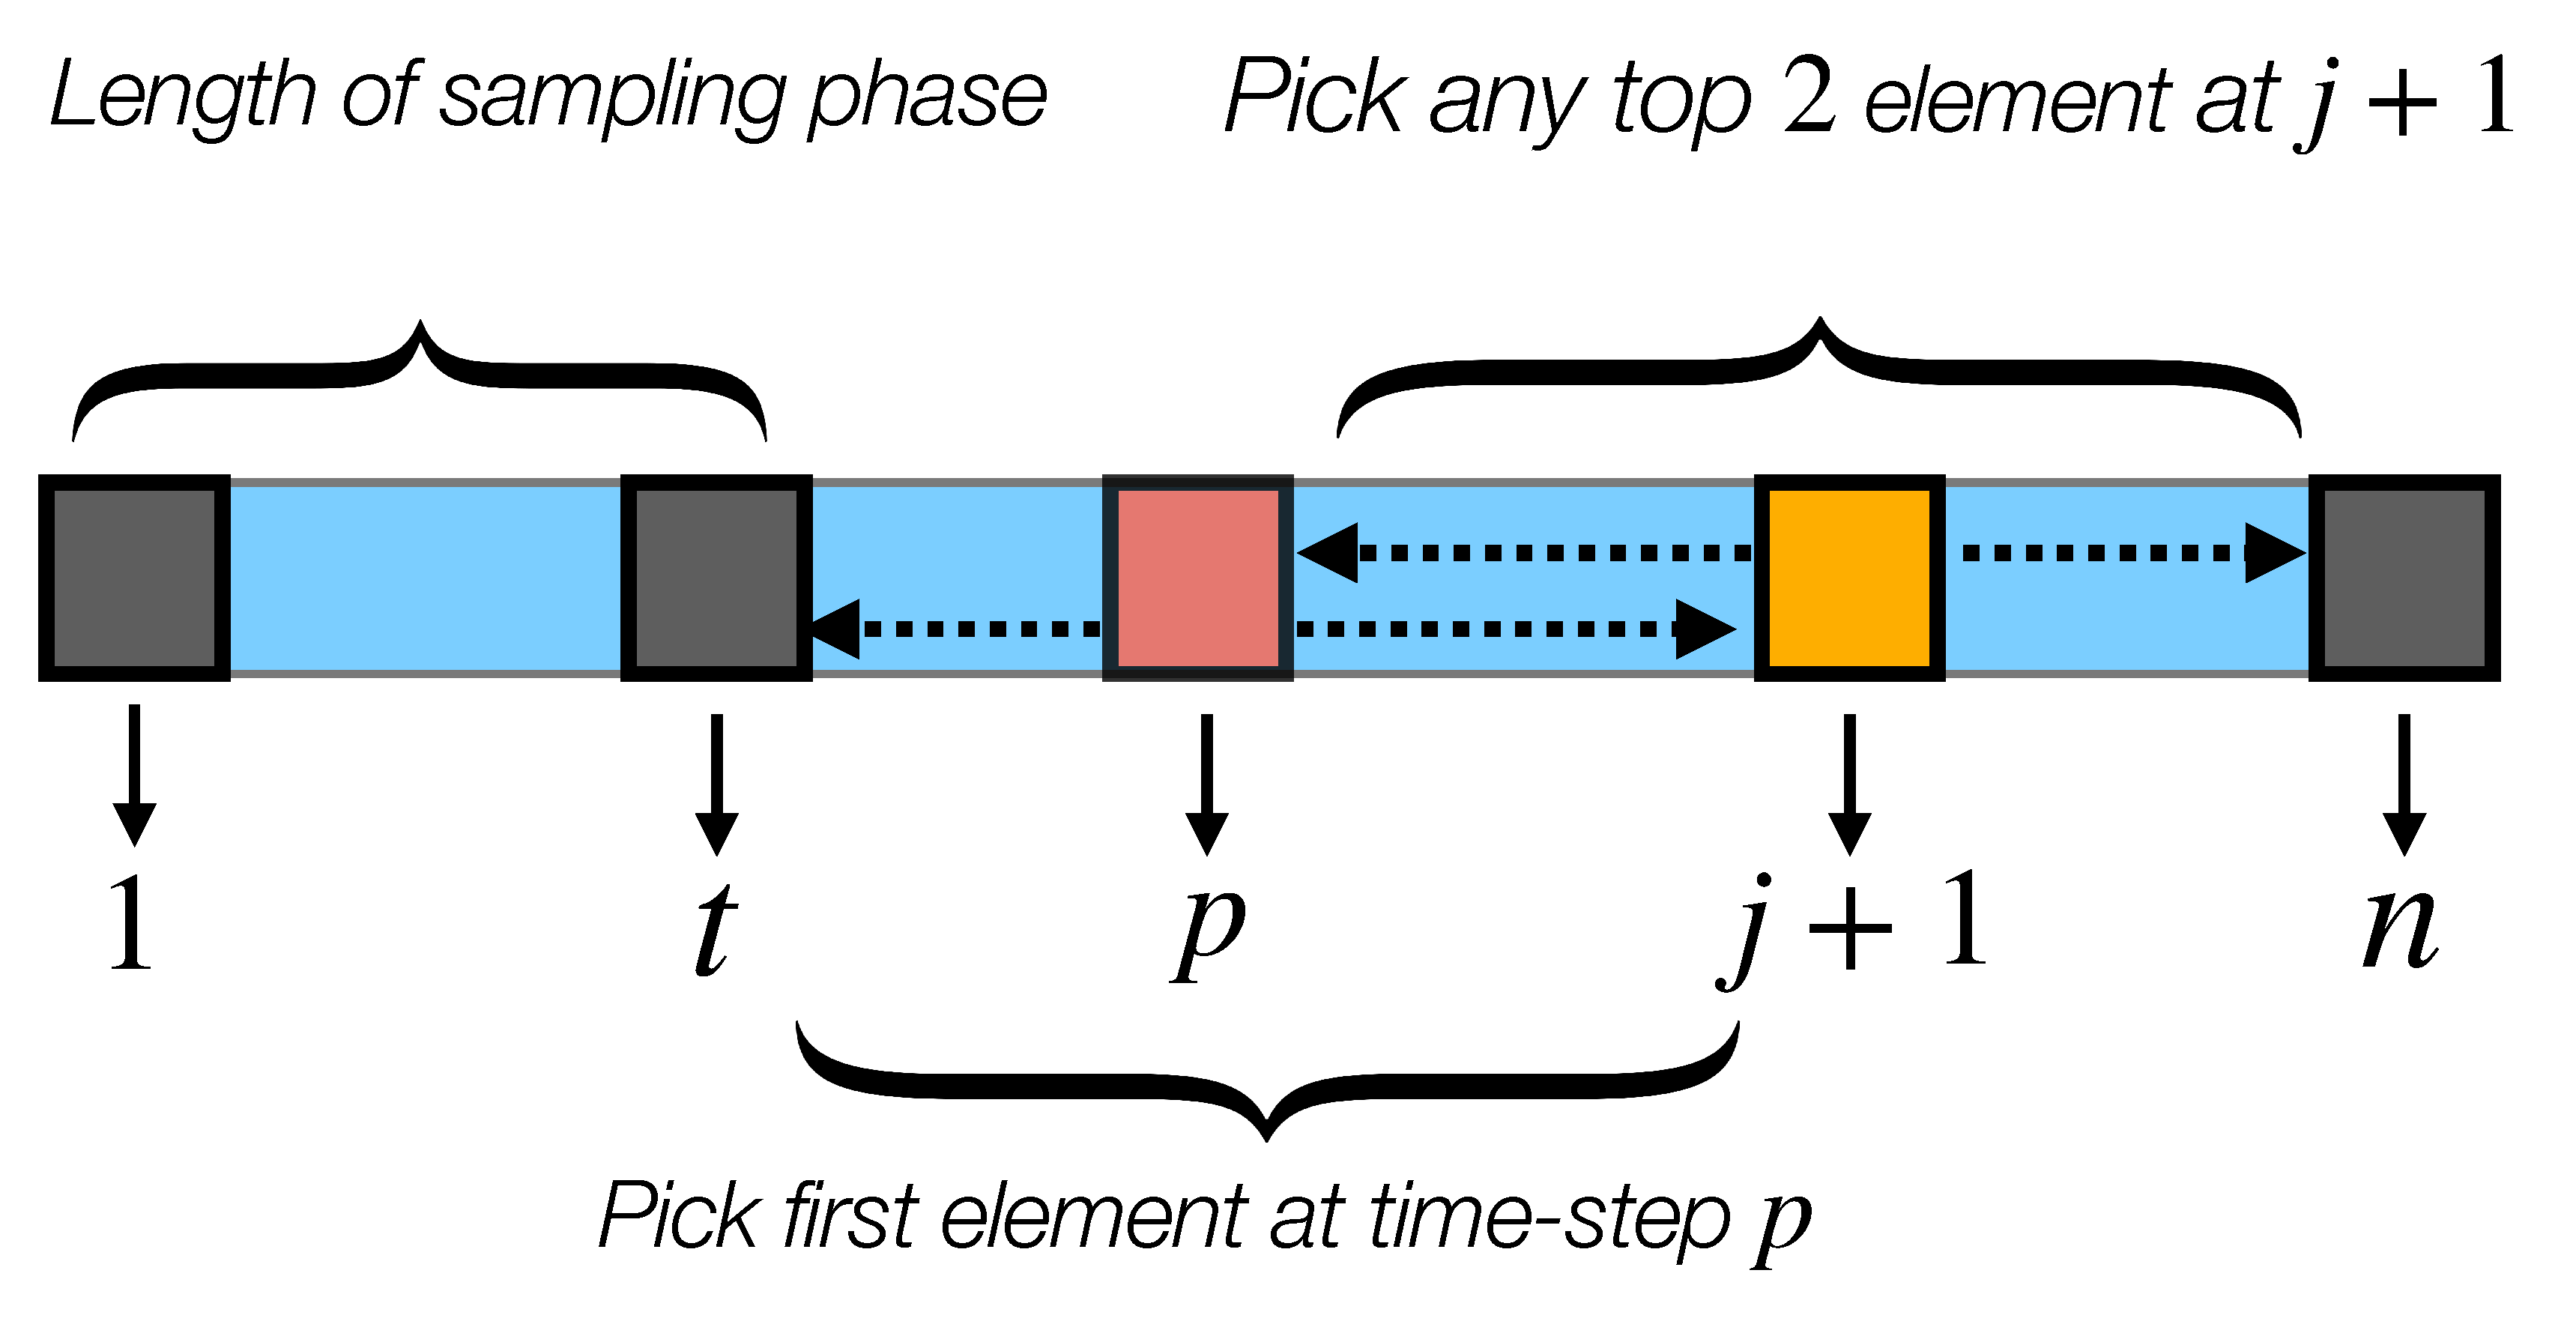
\includegraphics[width=1.0\linewidth]{Figures/virtual_plus_k_2.pdf}
    %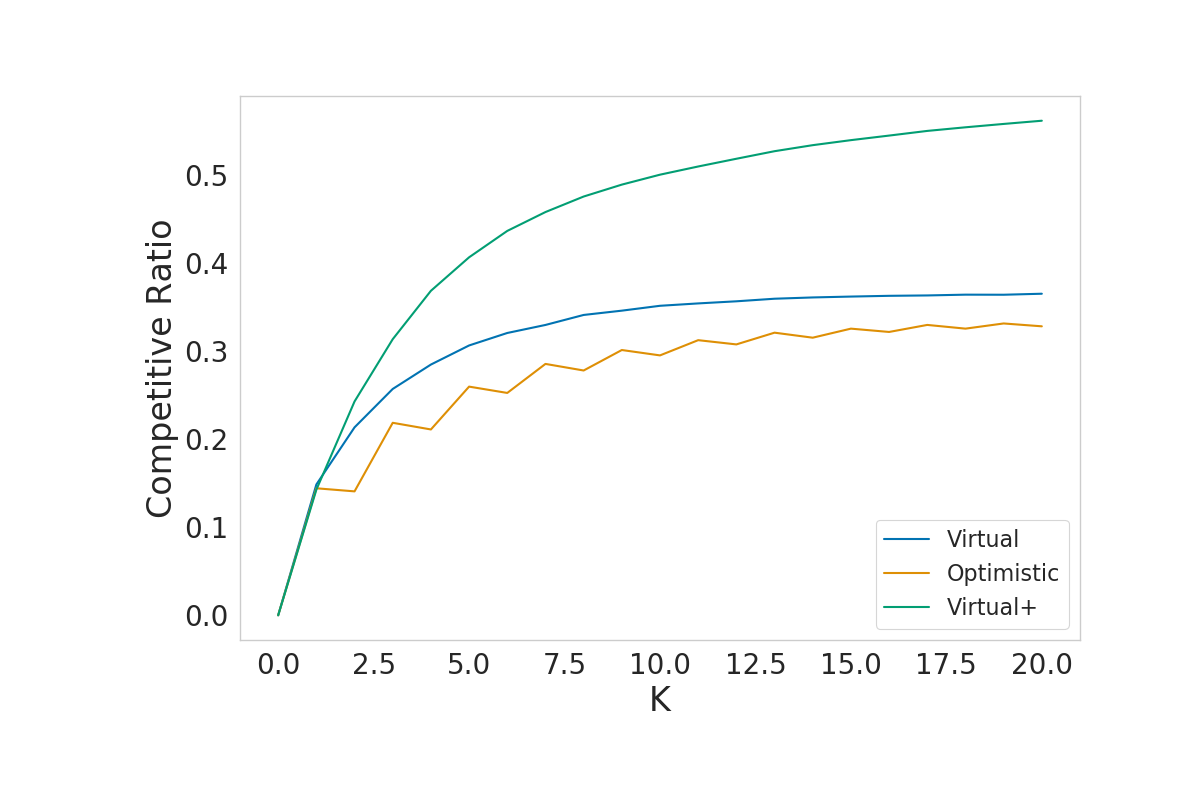
\includegraphics[width=\linewidth]{Figures/Competitive_RatioVar5.png}
    \caption{Probability of having only one element in $S_{\mathcal{A}}$ after $j$ time-steps with the \algoname\ algorithm.}
    \label{fig:k_2}
    \vspace{-15pt}
\end{figure}

\begin{proof}
First note that we can show that the competitive ratio for the $k$-secretary problem is equal to 
\begin{equation}
    C = \frac{1}{k}\sum_{a=1}^k \mathbb{P}(i_a \in S_\mathcal{A}), \label{eq:C_as_sum_prob1}
\end{equation}
where $i_a$ is the index of the $a^{th}$ secretary picked by the offline solution ---i.e. $i_a$ is a top-$k$ secretary of $\mathcal{D}$. 
Now, let us focus on the case $k=2$.
When calculating the probability of either of the top two items in $\mathcal{D}$ being picked by the \algoname\ we must first compute the probability of one of the top-2 items being picked during the selection phase (time step $t+1 \dots n$). Now notice that \algoname\ picks an item at time step $j+1$ if and only if this is a top-2 item with respect to all of $\mathcal{D}$ and $|S_{\mathcal{A}}| \leq 2$ at time-step $j+1$. Let top-$2_j$ denote the two largest elements observed by $\mathcal{A}$ up to and inclusive of time step $j$. Thus, for $a \in \{1,2\}$, we have
\begin{align}
    \mathbb{P}(i_a \in S_\mathcal{A}) 
    &= \sum_{j=t}^{n-1} \mathbb{P}(i_a \in S_\mathcal{A} \text{ at time-step }j+1) \label{p_picked_equal_not_filled} \\
    &= \frac{1}{n}\sum_{j=t}^{n-1} \mathbb{P}(|S_{\mathcal{A}}| \leq 2 \text{ at time-step } j + 1) \notag
\end{align}

Now, we compute $\mathbb{P}(|S_{\mathcal{A}}| \leq 2 \text{ at time-step } j+1)$ by decomposing this probability into the following two events: A.) $|S_{\mathcal{A}}| = 0$ where the selection set is empty and B.) the event $|S_{\mathcal{A}}| = 1$ where exactly one item has been picked. We now analyze each event in turn.

\xhdr{Event A} In order for the event $|S_{\mathcal{A}}|=0$ to occur it implies that the algorithm does not select any items in the first $j$ rounds. This means both two top-$2_j$ elements must have appeared in the sampling phase. Thus the probability for this event is exactly $\frac{t(t - 1)}{j (j - 1)}$. 

\xhdr{Event B}
The second event is when $|S_{\mathcal{A}}|=1$ ---i.e. the algorithm picks exactly one element in the first $j$ rounds. The computation of this event is illustrated in Figure~\ref{fig:k_2}. Let's say that an element is picked at time step $p$. Now to compute the probability of Event B occurring we first make the following two observations:

\begin{enumerate}[label={\bf Observation \arabic*:}, topsep=0pt, parsep=0pt, leftmargin=69pt, itemsep=2pt]
    \item  In order for exactly one element to be picked at the time step $p \leq j$, this element must be one of the top-$2_j$ elements. Furthermore, this implies the other of the top-$2_j$ element ---i.e. the one not picked at $p$ must have appeared in the sampling phase. Note that if both top-$2_j$ elements appear after the sampling phase, the condition would be satisfied twice and two elements would be selected instead of exactly one, and if they both appeared during the sampling phase we return to Event A. As a result, the probability for this condition is given by $\frac{t}{j (j - 1)}$.  
    \item By observation 1. we know that the online algorithm $\mathcal{A}$ picks one of the top-$2_j$ at time step $p$ and the fact that the event under consideration is $|S_{\mathcal{A}}|=1$ the reference list $R$ from time step $p$ to $j+1$ must contain both top-$2_j$ elements. However, for $\mathcal{A}$ to pick \emph{only} at $p$ we also need to ensure that no elements are picked prior t to $p$. Therefore, before time step $p$ the reference list must contain  top-$2_{p}$ . Again by observation 1, we know that $R$ already contains one of the top-$2_j$ elements therefore we know it contains one of the  top-$2_p$ elements. Thus the probability of ensuring that the second  top-$2_p$ elements is also within $R$ by time step $p$ is $\frac{(t - 1)}{(p - 2)}$. Finally, since there are two top elements and they may appear in any order we must count the probability of Event B occurring twice.

\end{enumerate}


Overall we get:
\begin{equation}
    \frac{t(t - 1)}{j (j - 1)} + 2 \sum_{p = t + 1}^{j}\frac{1}{j}\frac{t}{j - 1}\frac{t-1}{p-2}
\end{equation}
Total probability:
\begin{align*}
    \frac{1}{n} \sum_{j = t}^{n-1}\left(\frac{t(t - 1)}{j (j - 1)} + 2 \sum_{p = t + 1}^{j}\frac{1}{j}\frac{t}{j - 1}\frac{t-1}{p-2}\right) 
    &= 
   \frac{1}{n}\sum_{j = t}^{n-1}\left(1 + 2\sum_{p=t}^{j - 1} \frac{1}{p - 1} \right) \\
   &= 
   \frac{t(t - 1)}{n}\sum_{j=t}^{n-1}\left(\frac{1}{j(j-1)} + \frac{2}{j(j-1)}\sum_{p = t}^{j-1}\frac{1}{p-1}\right)\\
   & >
   \frac{t(t-1)}{n}\sum_{j = t}^{n - 1}\left(\frac{1}{j^2} + 2\frac{1}{j^2}\sum_{p = t + 1}^{j}\frac{1}{p-1}\right) \\
   & >
   \frac{t(t-1)}{n}\sum_{j = t}^{n - 1}\left(\frac{1}{j^2} + \frac{2}{j^2}\int_{p=t+1}^{j+1} \frac{1}{p-1}\, dp \right)\\
   & >
   \frac{t(t-1)}{n}\sum_{j = t}^{n-1}\left(\frac{1}{j^2} + \frac{2}{j^2}\ln\left(\frac{j}{t}\right)\right)
%   =\frac{t(t-1)}{n}(\sum_{j = t}^{a}(\frac{1}{j^2} + \frac{2}{j^2}\ln(\frac{j}{t})) + \sum_{j = a + 1}^{n - 1}(\frac{1}{j^2} + \frac{2}{j^2}\ln(\frac{j}{t})))\\
%   &\textgreater
%   \frac{t(t-1)}{n}(\int)
%   | \int_n^{n+1} f(t) dt - f(n)| \leq \int |f(t) - f(n)| dt \leq \int sup_{[n,t]}|f'(x)||t-n| dt
\end{align*}
Now we will use the following lemma
\begin{lemma}
For any differentiable function $f$ and any $a<b$, we have,
\begin{equation}
    \sum_{j=a}^{b} f(j) \geq \int_a^{b+1} f(t) dt - |b+1-a|\sup_{t \in [a,b+1]} |f'(t)|
\end{equation}
\end{lemma}
\begin{proof}
\begin{equation}
     | f(n) - \int_n^{n+1} f(t) dt | \leq \int_n^{n+1} |f(n)-f(t)| dt \leq \sup_{t \in [n,n+1]} |f'(t)| 
\end{equation}
Thus, 
\begin{equation}
    f(n) \geq  \int_n^{n+1} f(t) dt - \sup_{t \in [n,n+1]} |f'(t)| 
\end{equation}
and by summing for $n = a \ldots b$ we get the desired lemma. 
\end{proof}
Applying this lemma to $f(x) = \frac{1+2\ln(x/t)}{x^2}\,, a = t$ and $b=n-1$, we get 
\begin{align}
    \frac{1}{n} \sum_{j = t}^{n-1}\frac{t(t - 1)}{j (j - 1)} + 2 \sum_{p = t + 1}^{j}\frac{1}{j}\frac{t}{j - 1}\frac{t-1}{p-2} 
    & > \frac{t(t-1)}{n}\sum_{j = t}^{n-1}\left(\frac{1}{j^2} + \frac{2}{j^2}\ln\left(\frac{j}{t}\right)\right) \\
    & \geq \frac{t(t-1)}{n}\left(\int_{t}^{n}  \frac{1+2\ln(x/t)}{x^2} dx - 2(n-t) \sup_{x \in [t,n]} \left| 
    \frac{4 \ln(x/t)}{x ^3}\right| \right) \notag \\
    & \geq  \frac{t(t-1)}{n}\left(\int_{t}^{n}  \frac{1+2\ln(x/t)}{x^2} dx - 2(n-t) \left| \frac{16}{3 t^3 e^4} \right| \right) \notag \\
    & = 
    \frac{t(t -1)}{n} \left(\frac{3}{t}-\frac{2\ln(n/t) + 3}{n} - 2(n-t) \left| \frac{16}{3 t^3 e^4} \right|\right) 
\end{align}
Now for $t = \alpha n$ where $\alpha \in (0, 1)$ and as $n \xrightarrow[]{} \infty$, that lower-bound becomes 
\begin{equation}
C \geq \alpha (3 - \alpha(3 - 2\ln (\alpha))) + \mathcal{O}(1/n) \,,\quad \forall \alpha \in (0,1)
\end{equation}
The constant term of the RHS is a concave function of $\alpha$ that is maximized for $\alpha^* \approx 0.38240$. Thus, our algorithms achieves competitive ratio larger than $0.42737$.
\end{proof}


\clearpage

\section{Competitive Ratio General $k$}
\label{app:general_k_proof}
We now prove our main result for the competitive ratio of \algoname \ for $k \geq 2$. The theorem statement is reproduced here for convenience.  
\begin{reptheorem}{thm:general_k_theorem1}
The competitive ratio of \algoname\ for $k \geq 2$ and where $t = \alpha n$ can asymptotically be lower bounded by 
\begin{equation}
    C_k >  \max_{\alpha \in [0,1]}  {\alpha}^k \left(\sum_{m = 0}^{k - 1} a_m \ln^m (\alpha)\right) - \alpha a_0
    \hspace{0.15cm }where  \hspace{0.15cm }
    a_m = \left(\frac{\frac{k^k}{(k-1)^{k-m}} - k^m}{m!}\right)(-1)^{m+1}
    \, .
\end{equation}

\end{reptheorem}
\begin{figure}[ht]
    \centering
    %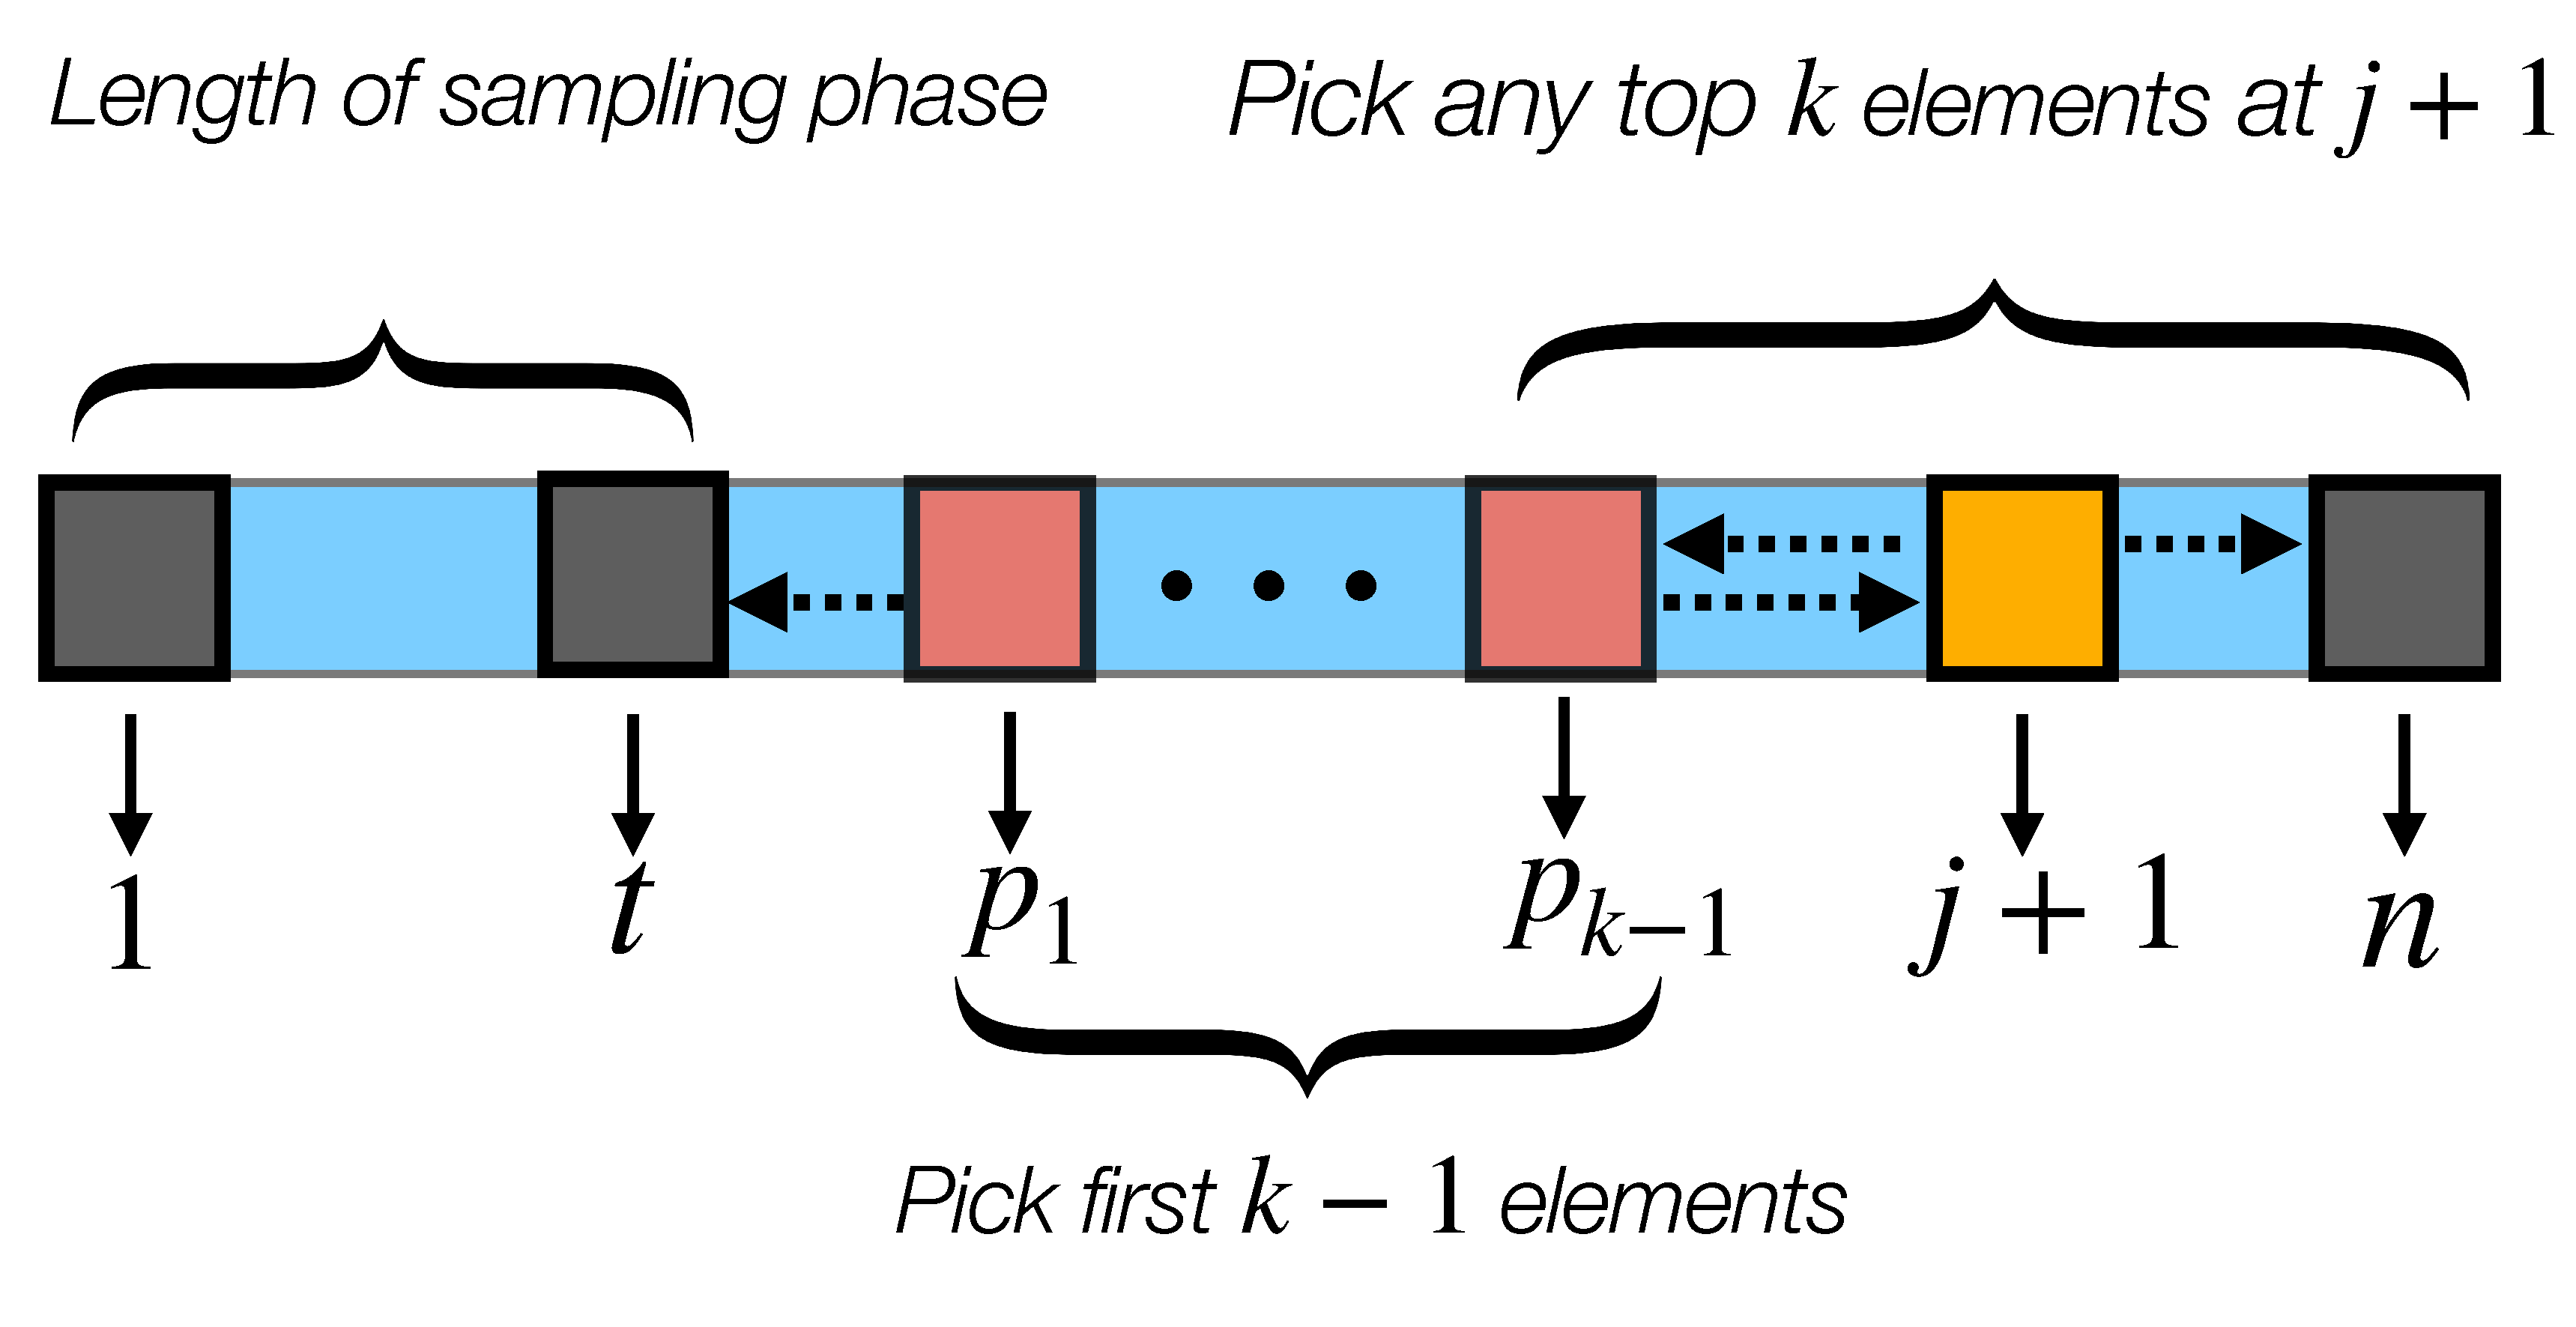
\includegraphics[width=0.50\linewidth]{Figures/virtual_plus_general_k.pdf}
    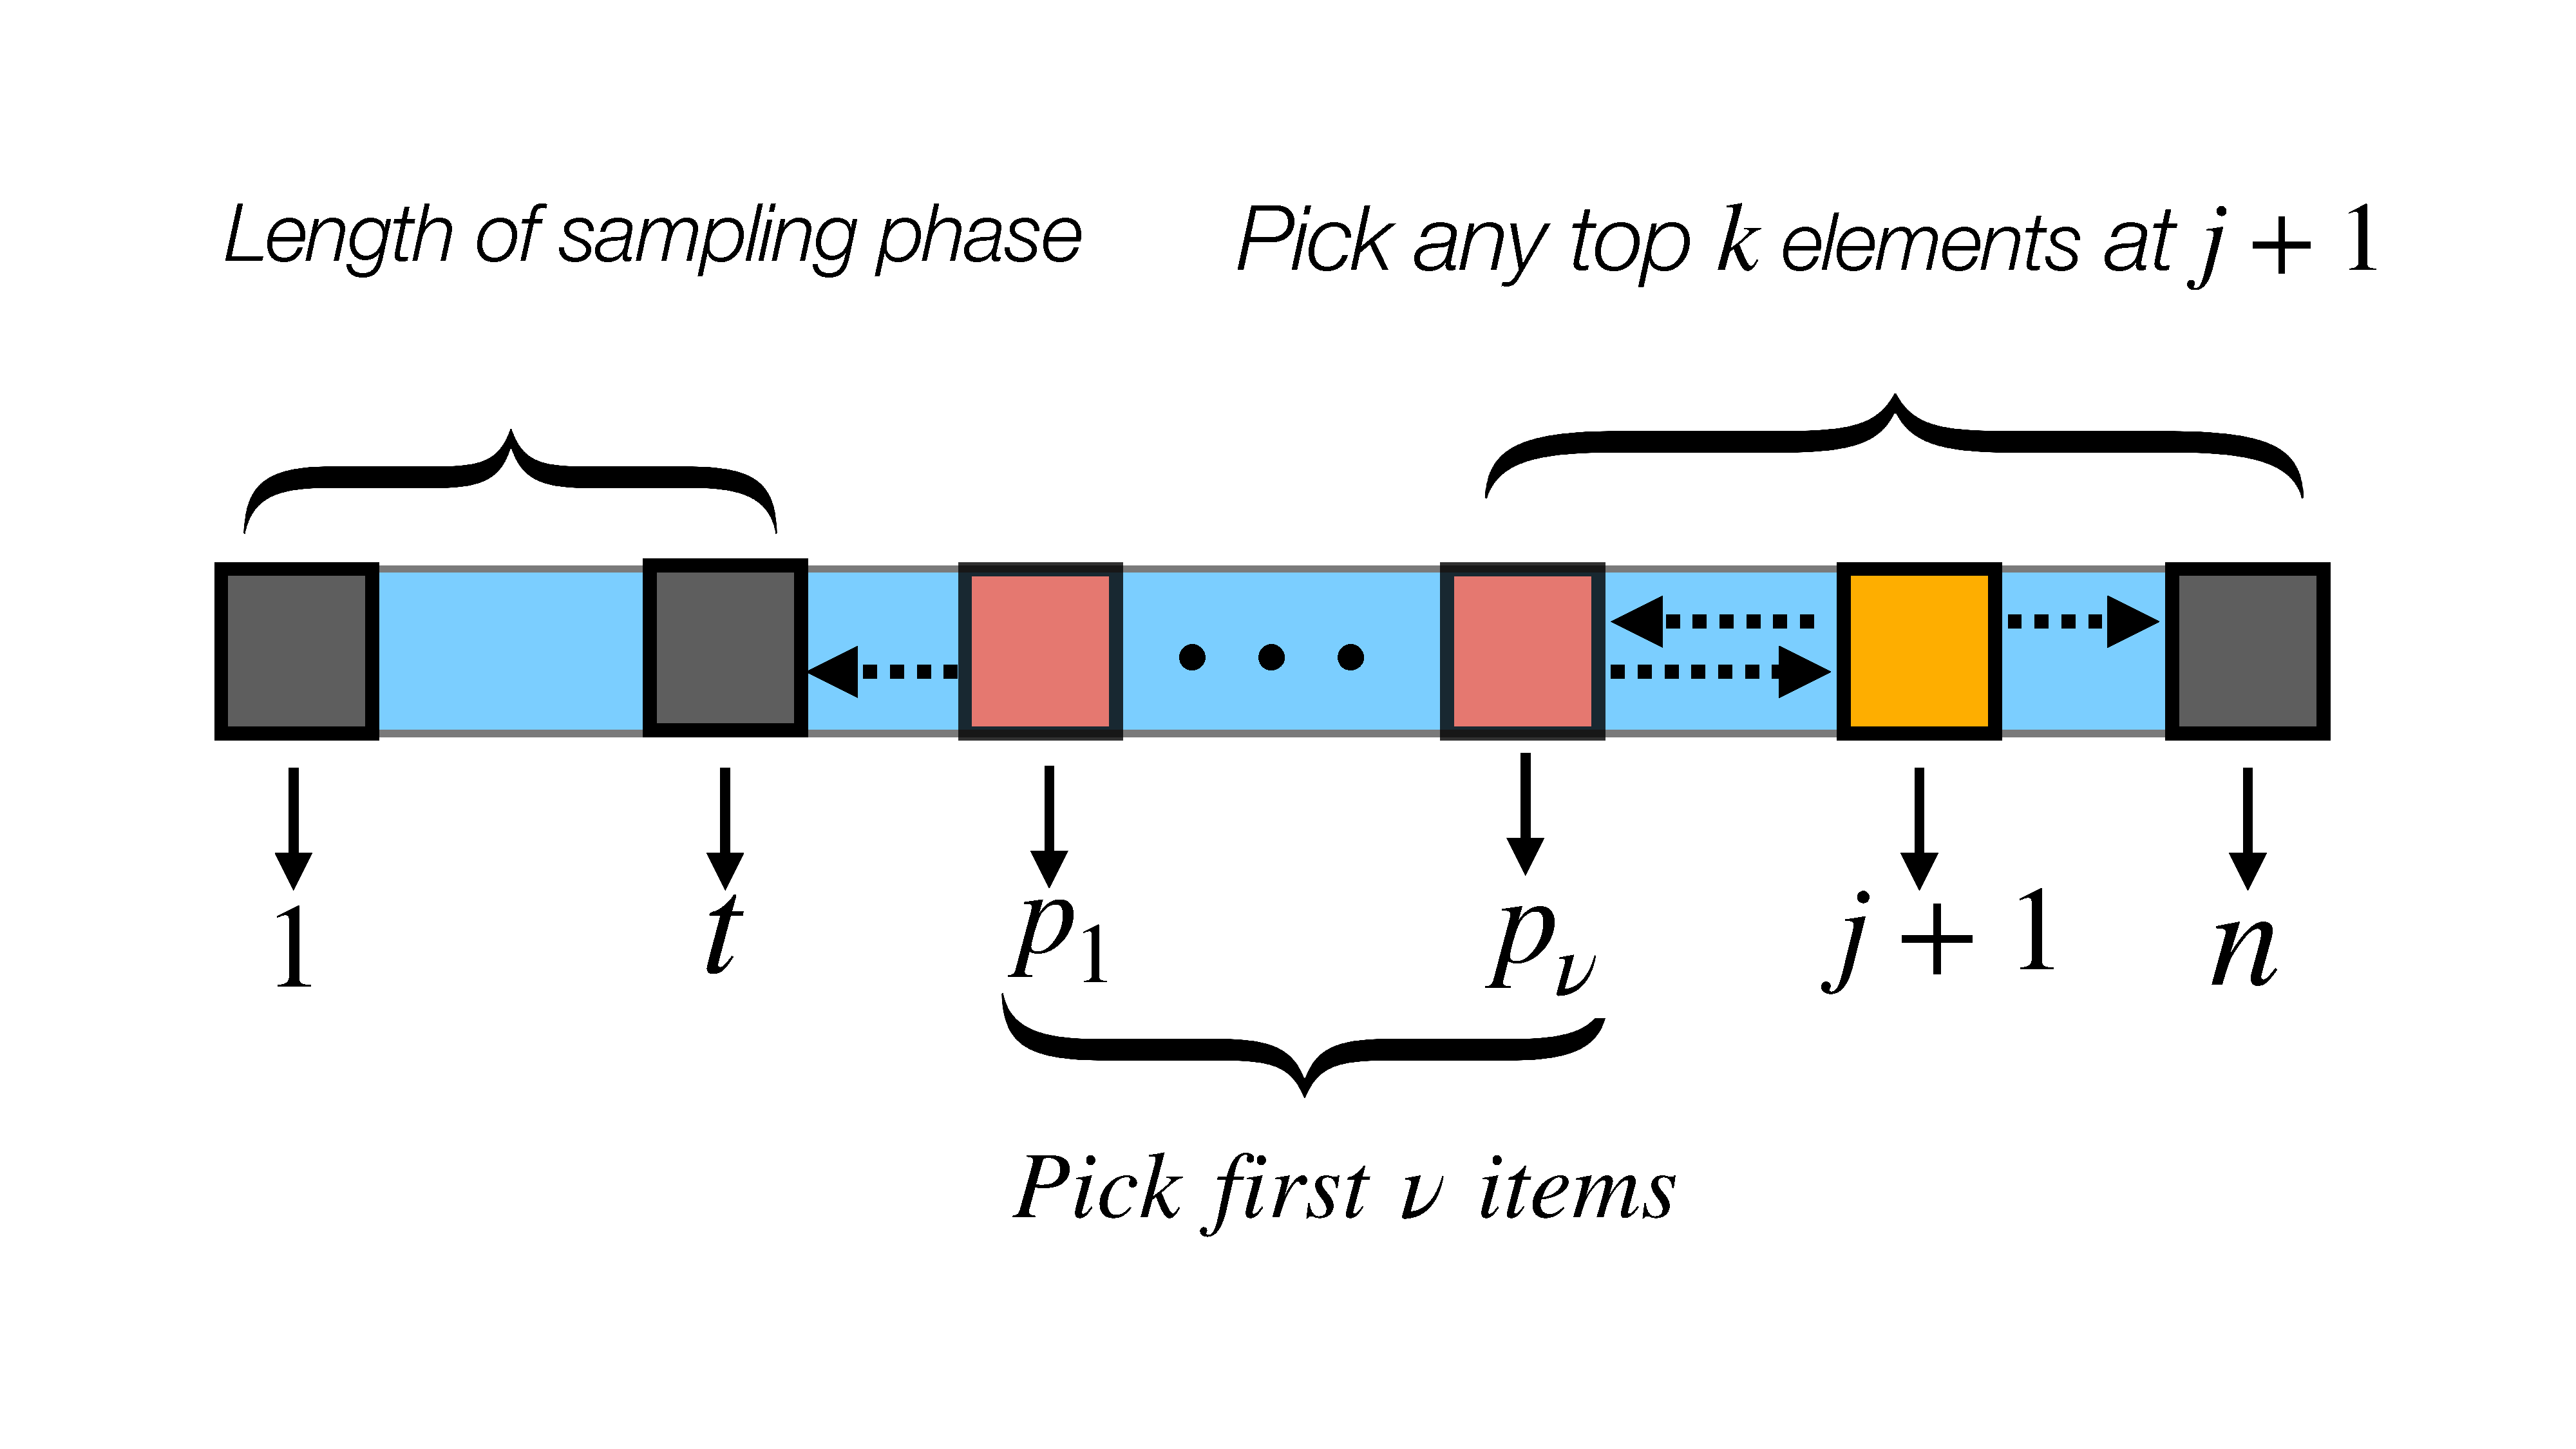
\includegraphics[width=1.0\linewidth]{Figures/general_k.pdf}
    %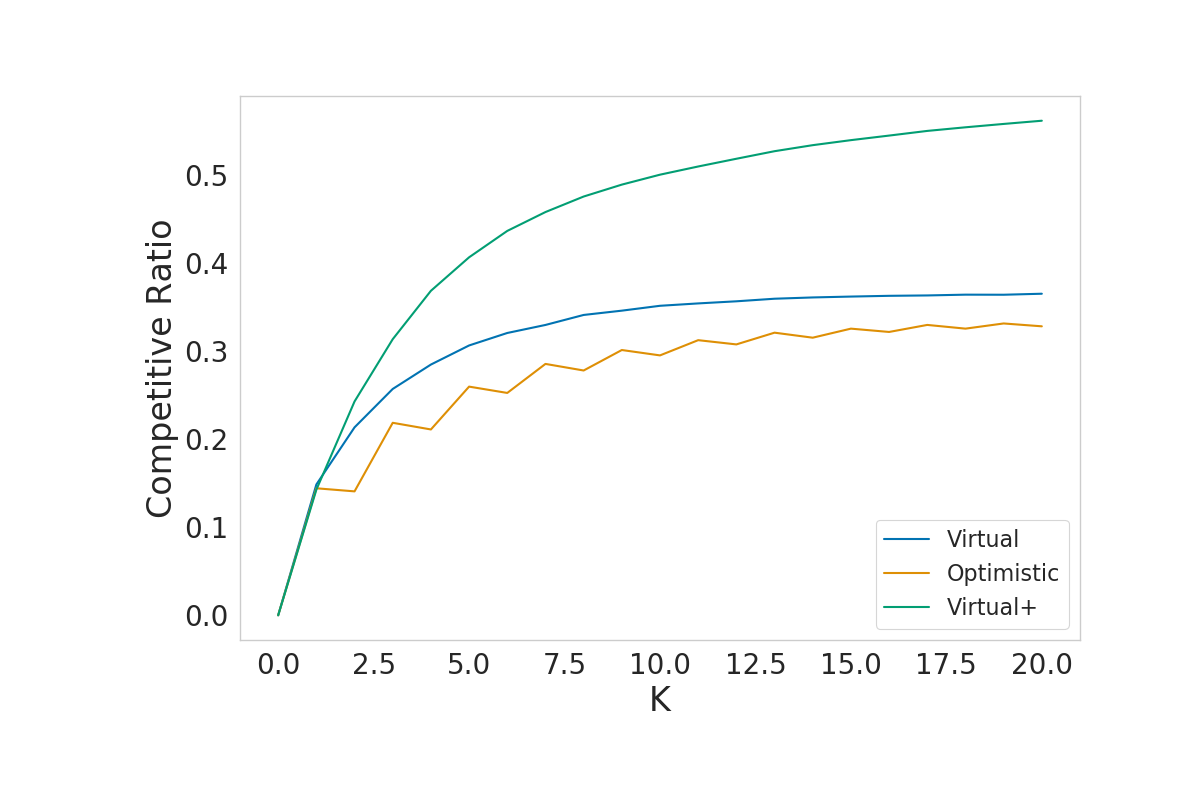
\includegraphics[width=\linewidth]{Figures/Competitive_RatioVar5.png}
    \caption{Virtual+ $k \geq 2$ proof.}
    \label{fig:general_k}
    \vspace{-15pt}
\end{figure}
\begin{proof}
First note that by \citet[Lemma 3.3]{albers2020new} we can show that the competitive ratio for the $k$-secretary problem for a monotone algorithm is equal to 
\begin{equation}
    C = \frac{1}{k}\sum_{a=1}^k \mathbb{P}(i_a \in S_\mathcal{A}), \label{eq:C_as_sum_prob1}
\end{equation}
where $i_a$ is the index of the $a^{th}$ secretary picked by the optimal offline solution ---i.e. $i_a$ is a top-$k$ secretary of $\mathcal{D}$. By Lemma \ref{lemma_monotone} \algoname \ is a monotone algorithm and we may use ~\eqref{eq:C_as_sum_prob1}.

\begin{align}
    \mathbb{P}(i_a \in S_\mathcal{A}) 
    &= \sum_{j=t}^{n-1} \mathbb{P}(i_a \in S_\mathcal{A} \text{ at time-step }j+1) \label{p_picked_equal_not_filled} \\
    &= \frac{1}{n}\sum_{j=t}^{n-1} \mathbb{P}(|S_{\mathcal{A}}| < k \text{ at time-step } j + 1) \notag
\end{align}

Now, we compute $\mathbb{P}(|S_{\mathcal{A}}| < k \text{ at time-step } j+1)$ by decomposing this probability into smaller events  $\mathbb{P}(|S_{\mathcal{A}}| = \nu \text{ at time-step } j+1)$ where $\nu \in [0,\dots,k-1]$.

We may compute the probability of $\mathbb{P}(|S_{\mathcal{A}}| = \nu \text{ at time-step } j+1)$ in the following manner. First, let us consider the scenario where $\nu$ elements are selected by \algoname\ at time steps $p_1$, $p_2, \dots, p_{\nu}$. 
Now, in order for an element to be selected at position $p_\nu$ that element must be one of the top $k$ elements up to time-step $j+1$. Therefore we have a factor $k/j$ in our equation. Now, in order to guarantee that no elements are picked after the position $p_\nu$ we additionally need to ensure that the remaining top-$k$ up to $j+1$ elements appear before $p_\nu$ which results in a factor of ${p_{\nu} - 1 \choose k - 1}/{j-1 \choose k - 1}$. 
Similarly, we may recursively calculate the corresponding factor for each position $p_{\nu-1} \dots p_1$. However, we also need to guarantee that no elements are picked within the time interval $[t+1 \dots p_1-1]$
---i.e. before $p_1$. The probability for this occurring is then ${t \choose k}/{p_1-1 \choose k}$ as this corresponds an ordering where the top-$k$ elements up to $p_1 - 1$ all appear in the sampling phase.
Thus, the probability $p_{t,j}^{k,\nu}:=\mathbb{P}(|S_{\mathcal{A}}| = \nu \text{ at time-step } j+1)$ is :
\begin{align}
    p_{t,j}^{k,\nu}
    &= \sum_{t+1 \leq p_1 < p_2 < \dots <p_{k-1} \leq j}\frac{k}{j} \frac{{p_{\nu} - 1 \choose k-1}}{{j-1 \choose k-1}}\frac{k}{p_{\nu} - 1}
    \frac{{p_{{\nu}-1} - 1 \choose k-1}}{{p_{\nu} - 2 \choose k-1}}\frac{k}{p_{\nu-1} - 1}\dots \frac{k}{p_2 - 1}\frac{{p_1 - 1 \choose k - 1}}{{p_2 - 2 \choose k-1}} \frac{{t \choose k}}{{p_1-1 \choose k}}\\
    & = \frac{t(t-1)\dots(t-k+1)}{j(j-1)\dots (j - k + 1)}\sum_{t+1 \leq p_1 < p_2 < \dots <p_{k-1} \leq j}
    \frac{k^{\nu}}{(p_\nu-k)(p_{\nu-1} - k)\dots(p_1 - k)}
\end{align}

Therefore, the probability of not exceeding $k$-selections, $p_{t,j}^k =\sum_{\nu=0}^{k-1} p_{t,j}^{k,\nu} $, to get before time step $j + 1$ is:
\begin{align}
   \notag
    & \frac{t(t - 1)...(t - k + 1)}{j (j - 1) \dots (j - k + 1)} \bigg(1 + k\hspace{-1em}\sum_{p_1 = t + 1\dots j}^{}\frac{1}{p_1 - k} + \dots
    + {k^{k - 1}}\hspace{-2em}\sum_{\substack{p_1 = t + 1 \dots p_2 - 1  \\\vdots\\ p_{k-1} = t + 1 \dots j}}\frac{1}{(p_1 - k)\dots (p_{k-1} - k)} \bigg)%%\\
    %& = 
    %\frac{t(t - 1)...(t - k + 1)}{j (j - 1) \dots (j - k + 1)} \bigg(1 + k\hspace{-0.5 em}\sum_{p_1 = t + 1}^{j}\frac{1}{p_1 - k} + 
     %\dots  +
     %{k^{k - 1}}\sum_{p_1 = t + 1}^{p_2 -1}\frac{1}{ (p_{1} - k)} \dots \sum_{p_{k-1} = t + 1}^{j}\frac{1}{ (p_{k-1} - k)} \bigg) 
\end{align}
Next, we make use of  
Lemma~\ref{lemma_three}:
\begin{align}
 p_{t,j}^{k} \geq 
     \frac{t(t - 1)\dots (t - k + 1)}{j(j - 1)\dots(j - k + 1)}\left(1 + \frac{k}{1!}\ln \Big(\frac{j - k}{t}\Big) +  \dots + \frac{k^{k - 1}}{(k-1)!}\ln^{k - 1}\Big(\frac{j - k}{t}\Big)\right)
\end{align}
Then we get that the total competitive ratio is: 
\begin{align}
     & \frac{1}{n}\sum_{j = t}^{n - 1}
     \frac{t(t - 1)\dots (t - k + 1)}{j(j - 1)\dots(j - k + 1)}\bigg(1 + \frac{k}{1!}\ln \Big(\frac{j - k}{t}\Big) +  \dots + \frac{k^{k - 1}}{(k-1)!}\ln^{k - 1}\Big(\frac{j - k}{t}\Big)\bigg)\\
     & \geq
     \frac{1}{n}\int_{j = t}^{n}
     \frac{t(t - 1)\dots (t - k + 1)}{j(j - 1)\dots(j - k + 1)}\bigg(1 + \frac{k}{1!}\ln \Big(\frac{j - k}{t}\Big) + \dots + \frac{k^{k - 1}}{(k-1)!}\ln^{k - 1}\Big(\frac{j - k}{t}\Big)\bigg)\\
     & \geq
     \frac{1}{n}\int_{j = t}^{n}
     \frac{t(t - 1)\dots (t - k + 1)}{j^k}\bigg(1 + \frac{k}{1!}\ln \Big(\frac{j - k}{t}\Big) + \dots + \frac{k^{k - 1}}{(k-1)!}\ln^{k - 1}\Big(\frac{j - k}{t}\Big)\bigg)
\end{align}
Now notice that:
\begin{equation}
    \label{identity_two}
    \int\frac{1}{a!} \frac{\ln^a(x)}{x^k} dx = - \frac{1}{x^{k - 1}}\sum_{m = 0}^{a}\frac{1}{m!}(k -1)^{m - 1 -a }\ln^m(x)
\end{equation}
Using the identity in ~\eqref{identity_two} we compute the competitive ratio as:
\begin{align}
     & \geq\frac{t(t - 1)\dots (t - k + 1)}{n}
     \bigg(\sum_{a = 0}^{k - 1}- \frac{1}{j^{k - 1}}{ k ^ a }\sum_{m = 0}^{a}\frac{1}{m!}(k -1)^{m - 1 -a }\ln^m\Big(\frac{j - k}{t}\Big) \bigg) \Big|_{j = t}^{n}\\
     & =
     \frac{t(t - 1)\dots (t - k + 1)}{n}\bigg(- \frac{1}{j^{k - 1}}\sum_{m = 0}^{k - 1}\frac{1}{m!}\Big(\sum_{a = m}^{k - 1}{k ^ a}(k - 1)^{m - a - 1}\Big)\ln^m{\Big(\frac{j - k}{t}\Big)}\bigg)\Big|_{j = t}^{n}
\end{align}
For threshold $t = \alpha n $ where $\alpha \in (0,1)$ and as $n \xrightarrow{}\infty$ our competitive rate becomes:
\begin{align}
    & \alpha \bigg(\sum_{a = 0}^{k - 1}{ k ^ a }{(k - 1)}^{-1 - a}\Big) - \alpha^k\Big(\sum_{m=0}^{k - 1}\frac{1}{m!}\Big(\sum_{a = m}^{k - 1}{ k ^ a }(k - 1)^{m - a - 1}\Big)\ln^m\Big(\frac{1}{\alpha}\Big)\bigg)\\
    & = \alpha\left({\left(\frac{k}{k-1}\right)}^{k} - 1\right) - \alpha^k\left(\sum_{m-0}^{k-1}\left(\frac{\frac{k^k}{(k-1)^{k-m}} - k^m}{m!}\right)(-1)^{m+1}\ln^m(\alpha)\right)
\end{align}
\end{proof}
\begin{definition}
\label{monotone_defn}
An algorithm is called monotone if the probabilities of selecting items $i$ and $j$ satisfy $p_i \geq p_j$ whenever the item values $v_i > v_j$ holds for any two items.
\end{definition}

\begin{lemma}
\label{lemma_monotone}
\algoname \ is a monotone algorithm. 
\end{lemma}
\begin{proof}
    In order to prove that \algoname \ is monotone as defined in Definition \ref{monotone_defn} we must prove that $p_i \geq p_j$ (where $p_i$ is the probability of picking the item $i$) for any two items where $v_i > v_j$. Without loss of generality let us consider a decreasing ordering of $n$-elements based on their values ---i.e. $v_1 > v_{2} > \dots > v_n$. 
    
    
    
    We prove that $p_i \geq p_{i+1}$ for all $i \in [1, \dots, n-1]$ by showing that for each input sequence where $v_{i+1}$ is accepted, there exists a unique input sequence where $v_i$ is accepted. Let us consider a permutation $\pi$ where $v_{i+1}$ appeared and was accepted at time step $a$ while $v_i$ appeared at time step $b$. By swapping $v_i$ and $v_{i+1}$ we obtain a new permutation $\pi'$ where $v_i$ now appears at $a$ and $v_{i+1}$ at $b$. We now study the two following cases.
    
    \xhdr{Case 1: $a < b$}
    
    If $a < b$ notice that the reference set, $R$, and the selected set $S_{\mathcal{A}}$, are exactly the same at time step $a$ for both permutations $\pi$ and $\pi'$. Therefore, if $v_{i+1}$ was accepted at time step $a$ in permutation $\pi$ then $v_i$ will also be accepted at time step $a$ in permutation $\pi'$ since $v_i > v_{i+1}$.   

    \xhdr{Case 2: $a > b$}
    
    If $a > b$ notice that $R$---by definition of \algoname---at time step $a$ contains top-$k$ elements observed in the first $a-1$ time steps. 
    Now the $k$-th element in $R$ at time-step $a$ must satisfy,
    \begin{equation*}
        R^a_{\pi}[k] \geq R^a_{\pi'}[k],
    \end{equation*}
    where $R^a_{[\cdot]}[k]$ corresponds to the $k$-element in the reference set for a specific permutation at time step $a$. Hence, we know that $v_{i} > v_{i+1} \geq R^a_{\pi}[k] \geq R^a_{\pi'}[k]$ as $v_{i+1}$ was assumed to be picked.
    
    
    Furthermore, the $S_{\mathcal{A}}$ and $R$ is the same for permutations $\pi$ and $\pi'$ at time-step $b$. Now by our primary assumption that $v_{i+1}$ is picked at time-step $a>b$ in $\pi$ this means that $v_i$ must be  $v_i \geq R^b_{\pi}[k]$ since $v_i > v_{i+1}$. However, observe that $v_i$ and $R^b_{\pi}[k]$ cannot be consecutive in value as $v_{i+1}$ appears at time-step $a > b$ in permutation $\pi$. This implies that $v_{i+1}$ must also be selected at time step $b$ in permutation $\pi'$ since $v_i$ and $v_{i+1}$ are consecutive in value. By a similar argument based on consecutive order of values between time steps $a$ and $b$ precisely the same elements will be selected in both $\pi$ and $\pi'$. The argument that   $v_{i} > v_{i+1} \geq R^a_{\pi}[k] \geq R^a_{\pi'}[k]$ implies that if $v_{i+1}$ is selected in permutation $\pi$, $v_i$ will also be selected in permutation $\pi'$. The claim then follows by applying the inequality $p_i \geq p_{i+1}$ in an iterative fashion.
\end{proof}
\begin{lemma} 
\label{lemma_three}
Let $f_i \,, \,i = 1 \ldots k$ be decreasing positive functions then we have 
\begin{equation}
    \sum_{p_1=a_1}^{b_1} \ldots \sum_{p_k=a_k}^{p_{k-1}} f_1(p_1) \ldots f_k(p_k)
    \geq \int_{x_1=a_1}^{b_1+1} \ldots \int_{x_k = a_k}^{x_{k-1}+1}  f_1(x_1) \ldots f_k(x_k) dx_1\dots dx_k
\end{equation}
\end{lemma}
\begin{proof}
    The main proof step involves in first noticing that since the functions $f_i \,, \,i = 1 \ldots k$ are decreasing and are positive we have, 
    \begin{equation}
        f_1(p_1) \ldots f_k(p_k) \geq  f_1(p_1) \ldots  f_{k-1}(p_{k-1})\int_{x_k = p_k}^{p_k+1} f_k(x_k) dx_k
    \end{equation}
    Thus, by summing this inequality for $p_k= a_k \ldots p_{k-1}$, we get
    \begin{equation}
    \sum_{p_k=a_k}^{p_{k-1}} f_1(p_1) \ldots f_k(p_k)
    \geq  f_1(p_1) \ldots  f_{k-1}(p_{k-1})  \int_{x_k = a_k}^{p_{k-1}+1} f_k(x_k) dx_k
    \end{equation}
    Now, because the functions $f_i \,, \,i = 1 \ldots k$ are decreasing and positive we have, 
     \begin{align}
    \mathcal{S} 
    &= \sum_{p_k=a_k}^{p_{k-1}} f_1(p_1) \ldots f_k(p_k)\\
    &\geq  f_1(p_1) \ldots  f_{k-2}(p_{k-2})  \int_{x_{k-1} = p_{k-1}}^{p_{k-1}+1} f_{k-1}(x_{k-1})  \int_{x_k = a_k}^{p_{k-1}+1} f_k(x_k) dx_{k-1}dx_k \\
    &\geq f_1(p_1) \ldots  f_{k-2}(p_{k-2})  \int_{x_{k-1} = p_{k-1}}^{p_{k-1}+1} f_{k-1}(x_{k-1})  \int_{x_k = a_k}^{x_{k-1}} f_k(x_k) dx_{k-1}dx_k 
    \end{align}
    where for the last inequality we used the fact that $x_{k-1} \in [p_{k-1}, p_{k-1}+1]$.
    Finally, by summing for $p_{k-1} = a_{k-1} \ldots p_{k-2}$, we get,
    \begin{align}
    \sum_{p_{k-1}=a_{k-1}}^{p_{k-2}}\mathcal{S} &= \sum_{p_{k-1}=a_{k-1}}^{p_{k-2}} \sum_{p_k=a_k}^{p_{k-1}} f_1(p_1) \ldots f_k(p_k)\\
    &\geq f_1(p_1) \ldots  f_{k-2}(p_{k-2})  \int_{x_{k-1} = p_{k-1}}^{p_{k-1}+1} f_{k-1}(x_{k-1})  \int_{x_k = a_k}^{x_{k-1}} f_k(x_k) dx_{k-1}dx_k
    \end{align}
    Using a recursive argument we finally get,
    \begin{equation}
    \sum_{p_1=a_1}^{b_1} \ldots \sum_{p_k=a_k}^{p_{k-1}} f_1(p_1) \ldots f_k(p_k)
    \geq \int_{x_1=a_1}^{b_1+1} \ldots \int_{x_k = a_k}^{x_{k-1}+1}  f_1(x_1) \ldots f_k(x_k) dx_1\dots dx_k
\end{equation}
\end{proof}


\clearpage
\subsection{Analytic computation of $C_k$ for \algoname}

\begin{table}[ht!]
    \centering
    \caption{Values of the Competitive ratio $C_k$ and the associated optimal $\alpha_k$ needed to compute the threshold for \algoname. Note that for $5\leq k\leq 100$ the competitive ratio of \textsc{Single-Ref} provided by~\citet{albers2020new} outperforms \algoname's competitive ratio. However, our analysis provides a tractable way to scale the analytic computation of the competitive ratio with $k$ as the function to optimize (and its gradients) in Theorem~\ref{thm:general_k_theorem1} is $\mathcal{O}(k)$.}
    \vspace{2pt}
    \begin{tabular}{ccccccccccc}
     \toprule
          $k$ & 2 &3 & 4 & 5 & 100 & 200 &300 &400 & 500 & 600\\
         \midrule
        $C_k$ & .4273&.4575&.4769&.4906&.5959&.6062&.6108&.6136&.6156&.6170 \\
        $\alpha_k$ & .3824 &.3867&.3884&.3890&.3781 &.3755 &.3743&.3735&.3729&.3726 \\
        \bottomrule
    \end{tabular}
    \label{tab:C_k}
\end{table}

\section{Proof of Theorem~\ref{thm:stochastic_secretary}}
\label{appendix:proof_thm2}
We now prove Theorem \ref{thm:stochastic_secretary} in detail, reproduced here for convenience. 

\begin{reptheorem}{thm:stochastic_secretary}
Let us consider a secretary algorithm, $\mathcal{A}$, that is $C_n$-competitive when given access to the true values $v_i, \,i \in [n]$. When having access to independent random variables $\mathcal{V}_{i},\, i\in [n]$ such that Eq.~\ref{eq:concentration} holds, $\mathcal{A}$ has a stochastic competitive ratio of at least:  
\begin{equation}
    C_n \left( 1-e^{- \frac{\Delta}{2 \sigma^2}} \right)^{\frac{-2 \exp(- \frac{\Delta}{2 \sigma^2})}{1 -  \exp(\frac{-\Delta}{\sigma^2})}}
\end{equation}
\end{reptheorem}

\begin{proof}
In this analysis, we will refer to a deterministic online algorithm as $\mathcal{A}$. Please note, the following statement of results holds for \textit{any} online algorithm, therefore when introducing certain lemmas we will use algorithm $\mathcal{A}$ for the name. Furthermore, we will denote the stochastic versions of $\mathcal{A}$ as $\mathcal{A}^{s}$.
Let $v_1^*, v_2^*, \dots v_k^*$ be the values of top $k$ elements and let $i_1^*, i_2^* \dots i_k^*$ be their appropriate indices. Therefore, the optimal offline solutions selects set 
$S^* = \{i_1^*, i_2^*, \dots i_k^*\}$, while a deterministic online algorithm $\mathcal{A}$ chooses set $S$, and our online algorithm $\mathcal{A}^{s}$ chooses set $S^{(s)}$. Our goal is to provide a lower bound of the kind
\begin{equation}
     \frac{\mathbb E[|S^{(s)} \cap S^*|]}{k} \geq c\frac{\mathbb E[|S \cap S^*|]}{k}
\end{equation}
where $c>0$ is a constant that depends on the randomness of the estimates $\mathcal{V}_i\,,i=1,\ldots,n.$ 
Assuming that $\mathcal{A}$ is $C_n$-optimal, this lower bound will provide us a competitive ratio for the stochastic algorithm $\mathcal{A}^{s}$.

% 
% Note that for any two random variable $X_i$ and $X_j$ for which we know that $\omega_i > \omega_j$ holds:
% \begin{align*}
% \sP(X_i < X_j)  & = 
% \sP((X_i - \omega_i) - (X_j - \omega_j) < \omega_j - \omega_i)  \\ & =   \sP (\epsilon_i - \epsilon_j < -\Delta) \leq e^{\frac{-\Delta}{{2\sigma}^2}}
% \end{align*}
%  therefore
%  \begin{equation}\label{equ:eight}
%  \sP(X_i > X_j) \geq (1 -  e^{\frac{-\Delta}{{2\sigma}^2}})
% \end{equation}


Now, by definition, the algorithm $\mathcal{A}^{s}$, is the algorithm $\mathcal{A}$ but operating on the random variables $\mathcal{V}_1, \mathcal{V}_2, ...\mathcal{V}_n$ (instead of $v_1,\ldots, v_n$. Thus, is we call $i_a^{(s)}$ the index of the $a$ largest value among  $\mathcal{V}_1, \mathcal{V}_2, ...\mathcal{V}_n$ (note that $i_a^{(s)}$ is a random variable) we have that 
\begin{equation}
   \sP[i_a^* \in S] = \sP[i_a^{(s)} \in S^{(s)}|\mathcal{V}_1, \dots,\mathcal{V}_n]
\end{equation}
and thus, by summing over $a$ and taking expectation on all permutations and noting $\{i_1^{(s)},\ldots,i_k^{(s)}\} := S^*_s$
\begin{equation}
    \sE[|S^* \cap S|] = \sE[|S^*_s \cap S^{(s)}|  \; | \mathcal{V}_1, \ldots,\mathcal{V}_n]
\end{equation}
Now let us note that 
we have that the expected number indices in $S^*$ picked by $\mathcal{A}^{s}$ is larger than the expected number of indices in $S^*_s\cup S^*$, formally,
\begin{align}
    \sE[|S^* \cap S^{(s)}|]  \notag
    &\geq \sE[|S^* \cap S^{(s)} \cap S^*_s|] \notag \\
    &\geq \sE [ \mathbf{1}\{S^* = S^*_s\} \sE[|S^* \cap S^*_s|\,| \mathcal{V}_1, \ldots,\mathcal{V}_n]] \notag\\
    &= \sP(S^*=S^*_s) \sE[|S^* \cap S|]
\end{align}
% \begin{equation}
%      \sum_{a=1}^k \sP[i_a^* \in S^{(s)}]
%      \geq \sum
%      _{a=1}^k \sP[i_a^{(s)} \in S^{(s)} \text{ and } i_a^{(s)} \in S^*]
% \end{equation}
Now, notice that without loss of generality we can consider that $v_1 \geq \dots \geq v_n$. Let us call, $\bar v:= \frac{v_k + v_{k+1}}{2}$, if we have $\mathcal{V}_{i_a^*} \geq \bar v \geq \mathcal{V}_{i_b^*}$ for $1 \leq a \leq k < b \leq n$ then we will have $S^*=S^*_s$. Let us formally bound this probability,
\begin{align*}
    \sP(S^*=S^*_s) 
    &\geq \sP(\mathcal{V}_{i_1^*}, \ldots, \mathcal{V}_{i_k^*} \geq \ldots \geq \mathcal{V}_{i_{k+1}^*} , \ldots, \mathcal{V}_{i_n^*})  \\
     & \geq \sP(\mathcal{V}_{i_a^*} \geq \bar v \geq \mathcal{V}_{i_b^*}\,,\,1 \leq a \leq k < b \leq n) \\
    & \geq \sP(\mathcal{V}_{i_a^*} \geq v_a - (2(k-a)+1)\Delta\,,\,   v_b + (2(b-k)-1) \Delta \geq  \mathcal{V}_{i_b^*}\,,\,1 \leq a \leq k < b \leq n) \\
\end{align*}
where is the last inequality we used that because $\Delta = \tfrac{1}{2}\min_{1\leq i \neq j \leq  n } \{\mid v_i - v_j \mid \}
$ we have
\begin{equation}
    v_a - (2(k-a)+1)\Delta \geq \bar v \geq  v_b + (2(b-k)-1) \Delta \,, \quad \forall \, 1 \leq a \leq k < b \leq n \,.
\end{equation}
Finally, using that the random variable $\mathcal{V}_i$ are independents we have,
\begin{align*}
    \sP(S^*=S^*_s)      
    & \geq \sP(|\mathcal{V}_{i_a^*} - v_a| \leq  2|k+1/2-a|\Delta, \,a \in [n]) \\
    & = \prod_{a=1}^n \sP(|\mathcal{V}_{i_a^*} - v_a| \leq  2|k+1/2-a|\Delta) \\
    & \geq \prod_{i=1}^n  (1 - e^{\frac{-2|k+1/2-i|\Delta}{2\sigma^2}})
\end{align*}
Where for the last inequality we used the assumption that 
\begin{equation}
    \sP( |\mathcal{V}_i-v_i| \geq \epsilon) \leq e^{\frac{-\epsilon^2}{2\sigma^2}} \,,\,\forall i \in [n]\,.
\end{equation}

Finally, we will lower-bound $\sum_{i=1}^n\log (1 - e^{\frac{-2|k+1/2-i|\Delta}{2\sigma^2}})$ by using the fact that for any $x$ such that $0<x<a<1$, we have by concavity of the $\log$,
\begin{equation}
    \log(1-x) \geq \log(1-a) x \,.
\end{equation}
Thus,
\begin{align}
    \sum_{l=1}^n\log (1 - e^{\frac{-2|k+1/2-l|\Delta}{2\sigma^2}}) 
    & \geq \log(1-e^{- \frac{\Delta}{2 \sigma^2}}) \sum_{l=1}^n e^{\frac{-2|k+1/2-l|\Delta}{2\sigma^2}} \\
    & \geq -2\log(1-e^{- \frac{\Delta}{2 \sigma^2}}) e^{- \frac{\Delta}{2 \sigma^2}} \sum_{l=1}^{\infty} e^{\frac{-l\Delta}{\sigma^2}} \\
    & \geq -2\log(1-e^{- \frac{\Delta}{2 \sigma^2}}) \frac{e^{- \frac{\Delta}{2 \sigma^2}} }{1 -  e^{\frac{-\Delta}{\sigma^2}}}
\end{align}
Which finally gives us,
\begin{equation}
     \sP(S^*=S^*_s)    \geq \left( 1-e^{- \frac{\Delta}{2 \sigma^2}} \right)^{\frac{-2 \exp(- \frac{\Delta}{2 \sigma^2})}{1 -  \exp(\frac{-\Delta}{\sigma^2})}}
\end{equation}



Note that we could refine this bound by considering individual gaps $\Delta_i$ and constants $\sigma_i$ and consider $\frac{\Delta}{\sigma^2} = \min_{i \in [n]} \frac{\Delta_i}{\sigma_i}$.

\end{proof}


\clearpage


\section{Classical Online Algorithms for Secretary Problems}
\label{appendix:classical_online_algorithms}

All single threshold online algorithm described in this paper include: \textsc{Virtual}, \textsc{Optimistic} and \textsc{Single-Ref}. Each online algorithm consists of two phases ---\textbf{sampling phase} followed by \textbf{selection phase}--- and an optimal stopping point $t$ which is used by the algorithm to transition between the phases. We now briefly summarize these two phases for the aforementioned online algorithms. 

\xhdr{Sampling Phase - \textsc{Virtual}, \textsc{Optimistic} and \textsc{Single-Ref}}
In the sampling phase, the algorithms passively observe all data points up to a pre-specified time index $t$, but also maintains a sorted reference list $R$ consisting of the $k$ elements with the largest values $\mathcal{V}(i)$ seen. Thus the $R$ contains a list of elements sorted by decreasing value. That is $R[k]$ is the index of the $k$-th largest element in $R$ and $\mathcal{V}(R[k])$ is its corresponding value. The elements in $R$ are kept for comparison but are crucially \textit{not} selected in the sampling phase.

\subsection{\textsc{Virtual} Algorithm}

\xhdr{Selection Phase - \textsc{Virtual} algorithm}
Subsequently, in the selection phase, $i > t$, when an item with value $\mathcal{V}(i)$ is observed an irrevocable decision is made of whether the algorithm should select $i$ into $S$. To do so, the Virtual algorithm simply checks if the value of the $k$-th smallest element in $R$, $\mathcal{V}(R[k])$, is smaller than $\mathcal{V}(i)$ in addition to possibly updating the set $R$. The full Virtual algorithm is presented in Algorithm 1.

\begin{algorithm}[ht]
\textbf{Inputs:} $t\in[k\dots n-k]$, $R = \emptyset$, $S_{\mathcal{A}} = \emptyset$
\newline
\textbf{Sampling phase:} Observe the first $t$ data points and construct a list $R$ with the indices of the top $k$ data points seen.  $\texttt{sort}$ ensures: $ \mathcal{V}(R[1]) \geq \mathcal{V}(R[2]) \dots \geq \mathcal{V}(R[k]).$

\textbf{Selection phase (at time $i>t$):}

\begin{algorithmic}[1]
\IF {$ \mathcal{V}(i) \geq  \mathcal{V}(R[k])$
and $R[k] > t$} 
        \STATE $R$ = $\texttt{sort}\{R \cup \{i\} \setminus \{R[k]\}\}$ \hfill\COMMENT{// Update $R$ with element $i$ and also take out $R[k]$}
\ELSIF{ $ \mathcal{V}(i) \geq  \mathcal{V}(R[k])$
and $R[k] \leq t$}
        \STATE $R$ = $\texttt{sort}\{R \cup \{i\} \setminus \{R[k]\}\}$ \hfill\COMMENT{// Update $R$ with element $i$ and also take out $R[k]$}
        \STATE $S_\mathcal{A} = \{ S_\mathcal{A} \cup \{i \}\}$ \hfill\COMMENT{// Select element $i$}
\ENDIF 
\STATE
$i\gets i + 1$
\end{algorithmic}
 \caption{\textsc{Virtual Algorithm}}
\end{algorithm}


\subsection{\textsc{Optimistic} Algorithm}

\xhdr{Selection Phase - \textsc{Optimistic} algorithm}
In the optimistic algorithm, i is selected if and only if $\mathcal{V}(i) \geq \mathcal{V}(R[last])$. Whenever $i$ is selected, $R[last]$
is removed from the list
$R$, but no new elements are ever added to $R$. Thus, intuitively, elements are selected when they beat one of the remaining reference
points from $R$.
We call this algorithm “optimistic” because it removes the reference
point $R[last]$ even if $ \mathcal{V}(i)$ exceeds, say, $ \mathcal{V}(R[1])$. Thus, it implicitly assumes
that it will see additional very valuable elements in the future, which
will be added when their values exceed those of the remaining, more
valuable, $R[a]\,,\,a \in [k]$.


\begin{algorithm}[ht]
\textbf{Inputs:} $t\in[k\dots n-k]$, $R = \emptyset$, $S_{\mathcal{A}} = \emptyset$.

\textbf{Sampling phase (up to time $t$):} Observe the first $t$ data points and construct a list $R$ with the indices of the top $k$ data points seen. $\texttt{sort}$ ensures: $ \mathcal{V}(R[1]) \geq \mathcal{V}(R[2]) \dots \geq\mathcal{V}(R[k]).$
Set $last = k$, to be the index of the last element in $R$.

\textbf{Selection phase (at time $i>t$):}

\begin{algorithmic}[1]
\IF {$\mathcal{V}(i) \geq \mathcal{V}(R[last])$} 
        \STATE $R$ = $\{R \setminus \{R[last]\}\}$ \hfill\COMMENT{// Update $R$ by taking out $R[k]$}
        \STATE $S_\mathcal{A} = \{ S_\mathcal{A} \cup \{i \}\}$ \hfill\COMMENT{// Select element $i$}
        \STATE $last = last - 1$
\ENDIF 
$i\gets i + 1$
\end{algorithmic}
 \caption{\textsc{Optimistic Algorithm}}
\end{algorithm}

\subsection{\textsc{Single-Ref} Algorithm}
\xhdr{Selection Phase - \textsc{Single-Ref} algorithm}
In the \textsc{Single-Ref} algorithm, $i$ is selected if and only if $\mathcal{V}(i) \geq \mathcal{V}(R[r])$ and we haven't already selected $k$ elements. 
We call this algorithm single reference algorithm because we always compare incoming elements to one single reference element, that was determined in the sampling phase.

\begin{algorithm}[ht]
\textbf{Inputs:} $t\in[k\dots n-k]$, $R = \emptyset$, $S_{\mathcal{A}} = \emptyset$, $r \in [k]$ (reference rank)

 \textbf{Sampling phase (up to time $t$):} Observe the first $t$ data points and construct a list $R$ with the indices of the top $k$ data points seen. Let $s_r = R[r]$ be the $r$-th best item from the sampling phase.

\textbf{Selection phase (at time $i>t$):} 
\begin{algorithmic}[1]
\IF {$\mathcal{V}(i) \geq s_r$ and $ |S_{\mathcal{A}}| \leq  k$} 
        \STATE $S_\mathcal{A} = \{ S_\mathcal{A} \cup \{i \}\}$ \hfill\COMMENT{// Choose the first $k$ items better than $s_r$}

\ENDIF 

$i\gets i + 1$
\end{algorithmic}
 \caption{\textsc{Single-Ref Algorithm}}
\end{algorithm}

\clearpage
\section{Additional Experimental Results}
\label{appendix:additional_results}

\subsection{Additional Results on Synthetic Data}
\label{appendix:synthetic_additional_results}
We now provide additional results on Synthetic Data with varying levels of noise added to each item in $\mathcal{D}$. In particular, we investigate in figure \ref{fig:additional_results_synthetic_data} online algorithms in the face of no noise ---i.e. $\sigma^2 = 0$, $\sigma^2 = 1$, and $\sigma^2 = 5$ in addition to $\sigma^2 = 10$ reported in figure \ref{fig:synthetic_data}. The deterministic setting corresponds to $\sigma^2 = 0$ while $\sigma^2=1$ and $\sigma^2=1$ correspond to the stochastic setting as introduced in section \ref{stochastic_k_secretary}.

\begin{figure}[ht]
    \centering
    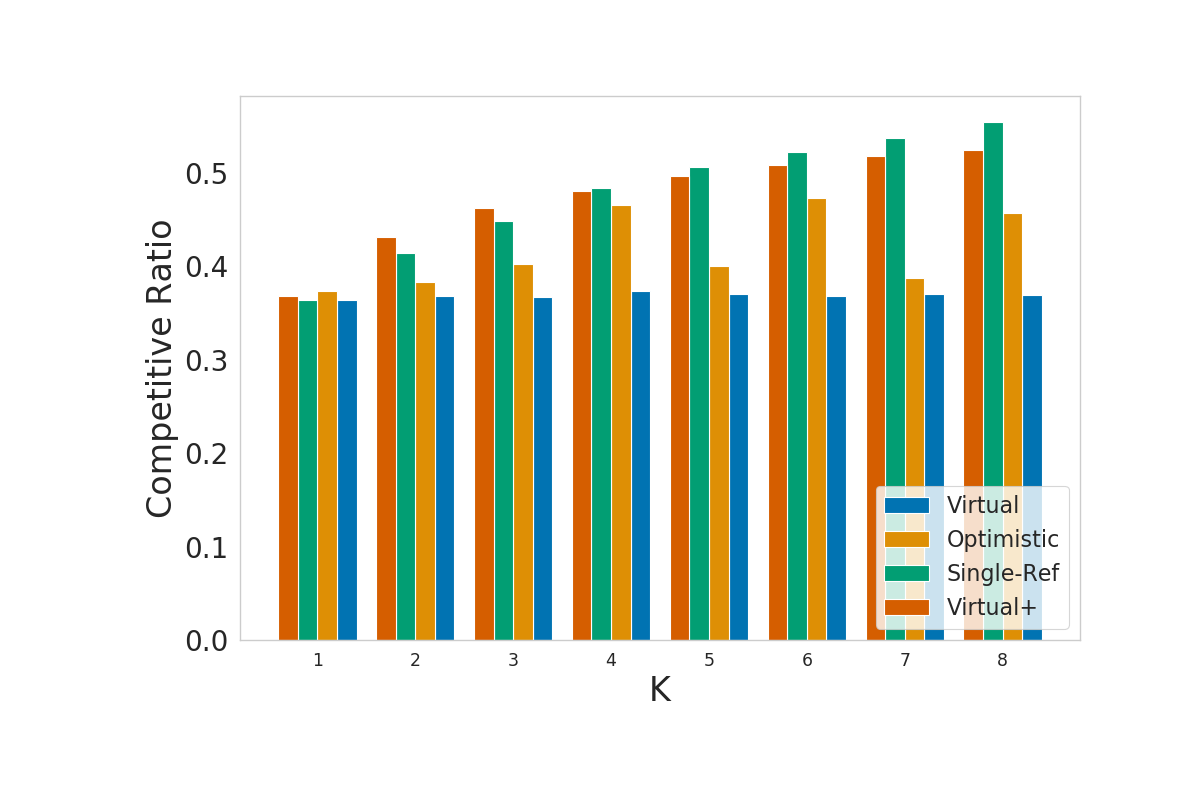
\includegraphics[width=0.32\linewidth]{Figures/Competitive_RatioBar8-Deterministic.png}
    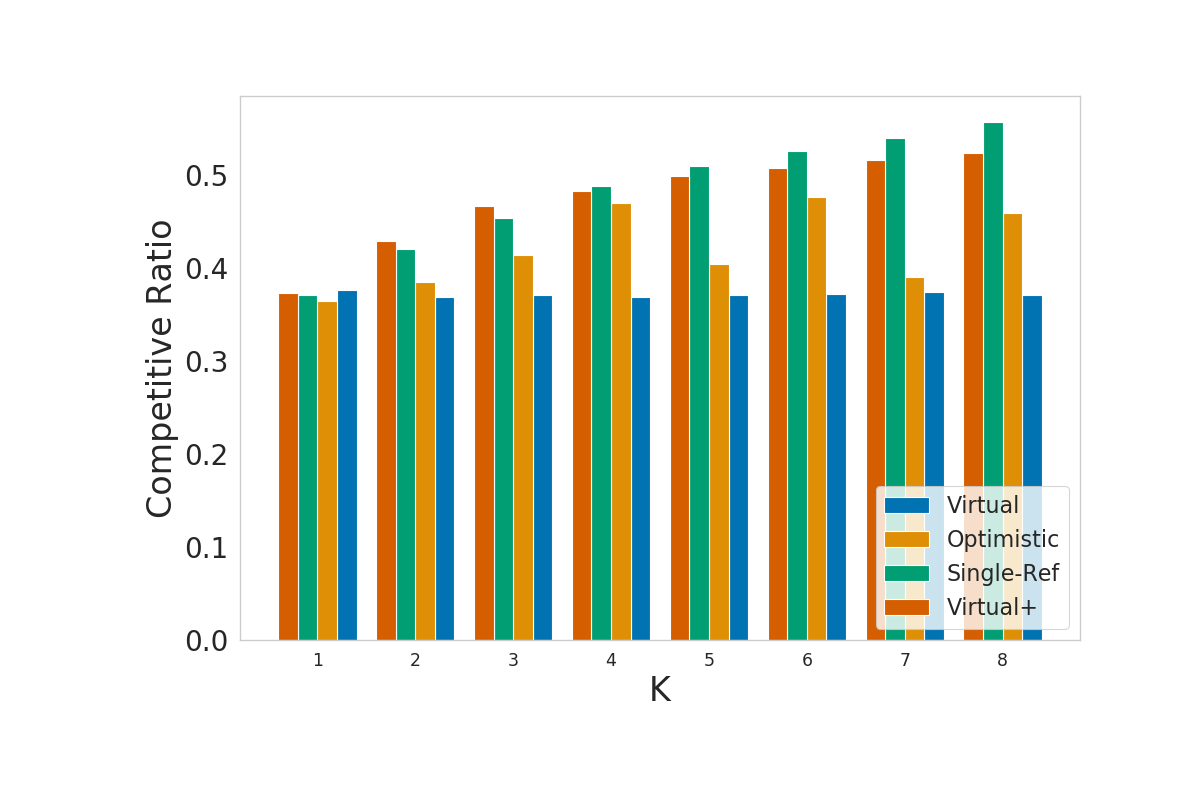
\includegraphics[width=0.32\linewidth]{Figures/Competitive_RatioBar8-Var-1.png}
    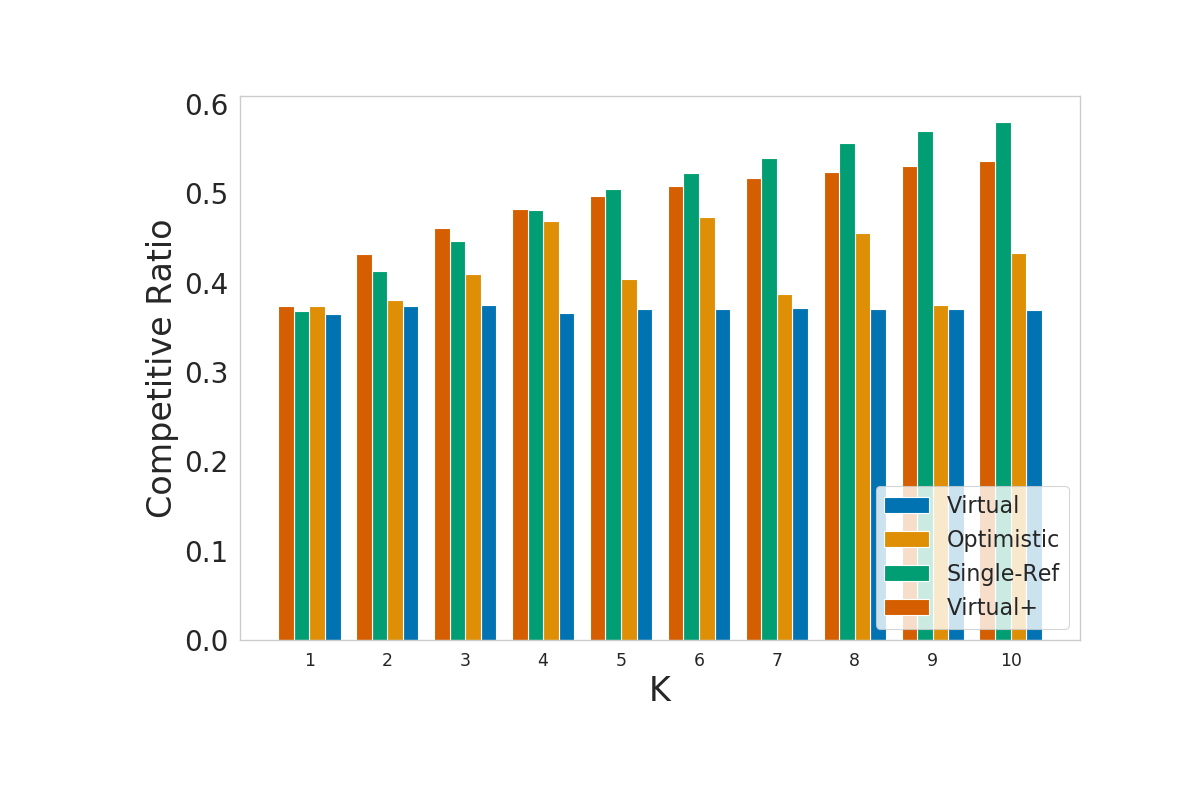
\includegraphics[width=0.32\linewidth]{Figures/Competitive_RatioBar-Var-5.png}
    \caption{Estimation of the competitive ratio of online algorithms under various noise levels. \textbf{Left:} Deterministic setting with $\sigma^2=0$. \textbf{Middle:} Stochastic setting with $\sigma^2 = 1$. \textbf{Right:} Stochastic setting with $\sigma^2 = 5$.}
    \label{fig:additional_results_synthetic_data}
\end{figure}




\subsection{Experimental Details}
\label{appendix:additional_results_larger_datasets}
We provide more details about the experiments presented in section~\ref{section:experiments}. For further details we also invite the reader to look at the code provided with the supplementary materials.

\paragraph{Attack strategies} We use two different attack strategies the Fast Gradient Sign Method (FGSM) \citep{goodfellow2014explaining} and 40 iterations of the PGD attack \citep{madry2017towards} with $l_\infty$.

\paragraph{Hyper-parameters of online algorithms} All the online algorithms except \textsc{Single-Ref} have a single hyper-parameters to choose which is the length of the sampling phase $t$. For \textsc{Virtual} and \textsc{Optimistic} we use $t=\floor{ \frac{t}{e}}$ which is the value suggested by theory in \citet{babaioff2007knapsack}. For \textsc{\algoname} we use $t=\alpha n$ as in Eq.~\ref{eq:alpha_eqn} which is the value suggested by Theorem~\ref{thm:K_2_theorem1}. \textsc{Single-Ref} has two hyper-parameters to choose the threshold $t$ ($c$ in the original paper) and reference rank $r$. For $k=1...100$ the values are given in \citet{albers2020new} and are numerical solutions to combinatorial optimization problems. However, for $k = 1000$ no values are specified and we choose $c=0.13$ and $r=40$ through grid search. Indeed, these values may not be optimal ones but we leave the choice of better values as future work.

\paragraph{MNIST model architectures} For table~\ref{table:non_robust_table1}, $f_s$ and $f_t$ are chosen randomly from an ensemble of trained classifiers. The ensemble is composed of five different architectures described in table~\ref{appendix:mnist_ens_adv_training_table}, with 5 trained models per architecture.

\begin{table}[h]
    \centering
          
            \begin{tabular}{ccccc}
            \toprule
                   &  A  & B  & C & D \\
                    \midrule
                   & Conv(64, 5, 5) + Relu & Dropout(0.2) & Conv(128, 3, 3) + Tanh & \multirow{2}{*}{\shortstack{FC(300) + Relu \\ Dropout(0.5)}}\\
                   & Conv(64, 5, 5) + Relu &  Conv(64, 8, 8) + Relu &  MaxPool(2,2) & \\
                   & Dropout(0.25) & Conv(128, 6, 6) + Relu  & Conv(64, 3, 3) + Tanh & \multirow{2}{*}{\shortstack{FC(300) + Relu \\ Dropout(0.5)}} \\
                   & FC(128) + Relu & Conv(128, 6, 6) + Relu & MaxPool(2,2) & \\
                   & Dropout(0.5) &  Dropout(0.5)  &  FC(128) + Relu &  \multirow{2}{*}{\shortstack{FC(300) + Relu \\ Dropout(0.5)}}\\
                   & FC + Softmax &  FC + Softmax &  FC + Softmax & \\
                   & & & & \multirow{2}{*}{\shortstack{FC(300) + Relu \\ Dropout(0.5)}} \\
                   & & & & \\
                   & & & & FC + Softmax \\
            \bottomrule
            \end{tabular}
            \caption{The different MNIST Architectures used for $f_s$ and $f_t$}
            \label{appendix:mnist_ens_adv_training_table}
    \end{table}

\paragraph{CIFAR model architectures} For table~\ref{table:non_robust_table1}, $f_s$ and $f_t$ are chosen randomly from an ensemble of trained classifiers. The ensemble is composed of five different architectures: VGG-16 \citep{simonyan2014very}, ResNet-18 (RN-18) \citep{he2016deep}, Wide ResNet (WR) \citep{zagoruyko2016wide}, DenseNet-121 (DN-121) \citep{huang2017densely} and Inception-V3 architectures (Inc-V3) \citep{szegedy2016rethinking}, with 5 trained models per architecture.

\subsection{Additional metrics}
In addition to the results provided in table~\ref{table:non_robust_table1}, we also provide two other metrics here: the stochastic competitive ratio in table~\ref{appendix:comp_ratio_non_robust} and the knapsack ratio table~\ref{appendix:knap_ratio_non_robust}. Where the knapsack ratio is defined as the sum value of $S_{\mathcal{A}}$ ---i.e. the sum of total loss, as selected by the online algorithm divided by the value of $S^*$ selected by the optimal offline algorithm.
We observe that the competitive ratio is not always a good metric to compare the actual performance of the different algorithms, since sometimes the online algorithm with the best competitive ratio is not the algorithm with the best fool rate. The knapsack ratio on the other hand seems to be a much better proxy for the actual performance of the algorithms, this is due to the fact that we're interested in picking elements that have have a good chance to fool the target classifier but are not necessarily the best possible attack.

\begin{table*}[ht]
\begin{small}
\caption{Competitive ratio on non-robust models using FGSM and PGD attacker and various online algorithms.}
\label{appendix:comp_ratio_non_robust}
 \begin{center}\begin{tabular}{ c c c c c c c c }
 \toprule
 & & \multicolumn{3}{c}{MNIST (competitive ratio)} & \multicolumn{3}{c}{CIFAR-10 (competitive ratio)}\\
 & Algorithm & $k=10$ & $k=100$ & $k=1000$ & $k=10$ & $k=100$ & $k=1000$ \\
 \midrule
 \multirow{6}{*}{FGSM}
 & \textsc{Naive} (Lower-bound) & .006 $\pm$ .001 & .010 $\pm$ .000 & .098 $\pm$ .000 & .002 $\pm$ .000 & .010 $\pm$ .000 & .100 $\pm$ .000\\
 \cmidrule{2-8}
 & \textsc{Optimistic} & .063 $\pm$ .004 & .083 $\pm$ .003 & .197 $\pm$ .003 & .035 $\pm$ .002 & .064 $\pm$ .001 & .203 $\pm$ .001\\
 & \textsc{Virtual} & .048 $\pm$ .003 & .079 $\pm$ .003 & .201 $\pm$ .003 & .030 $\pm$ .002 & .073 $\pm$ .001 & .212 $\pm$ .001\\
 & \textsc{Single-Ref} & .070 $\pm$ .004 & .135 $\pm$ .006 & .181 $\pm$ .003 & .045 $\pm$ .002 & .109 $\pm$ .002 & .174 $\pm$ .001\\
 & \algoname & .072 $\pm$ .004 & .124 $\pm$ .005 & .270 $\pm$ .005 & .043 $\pm$ .002 & .107 $\pm$ .002 & .287 $\pm$ .002\\
 \midrule
 \multirow{6}{*}{PGD}
 & \textsc{Naive} (lower bound) & .005 $\pm$ .001 & .010 $\pm$ .000 & .098 $\pm$ .000 & .001 $\pm$ .000 & .010 $\pm$ .000 & .100 $\pm$ .000\\
 \cmidrule{2-8}
 & \textsc{Optimistic} & .023 $\pm$ .002 & .036 $\pm$ .001 & .156 $\pm$ .001 & .033 $\pm$ .002 & .052 $\pm$ .002 & .157 $\pm$ .002\\
 & \textsc{Virtual} & .011 $\pm$ .001 & .049 $\pm$ .001 & .173 $\pm$ .001 & .028 $\pm$ .002 & .056 $\pm$ .002 & .160 $\pm$ .002\\
 &\textsc{Single-Ref} & .032 $\pm$ .002 & .067 $\pm$ .002 & .135 $\pm$ .001 & .042 $\pm$ .003 & .087 $\pm$ .003 & .145 $\pm$ .001\\
 & \algoname & .023 $\pm$ .002 & .059 $\pm$ .002 & .215 $\pm$ .002 & .040 $\pm$ .002 & .081 $\pm$ .003 & .200 $\pm$ .003\\
 \bottomrule
\end{tabular}\end{center} 
\end{small}
\end{table*}

\begin{table*}[ht]
\begin{small}
\caption{Knapsack ratio on non-robust models using FGSM and PGD attacker and various online algorithms.}
\label{appendix:knap_ratio_non_robust}
 \begin{center}\begin{tabular}{ c c c c c c c c }
 \toprule
 & & \multicolumn{3}{c}{MNIST (knapscak ratio in \%)} & \multicolumn{3}{c}{CIFAR-10 (knapsack ratio in \%)}\\
 & Algorithm & $k=10$ & $k=100$ & $k=1000$ & $k=10$ & $k=100$ & $k=1000$ \\
 \midrule
 \multirow{6}{*}{FGSM}
 & \textsc{Naive} (Lower-bound) & 19.0 $\pm$ 0.3 & 19.5 $\pm$ 0.2 & 29.9 $\pm$ 0.2 & 16.8 $\pm$ 0.2 & 20.3 $\pm$ 0.1 & 28.7 $\pm$ 0.1\\
 \cmidrule{2-8}
 & \textsc{Optimistic} & 33.0 $\pm$ 0.6 & 33.1 $\pm$ 0.3 & 42.1 $\pm$ 0.3 & 32.7 $\pm$ 0.4 & 34.1 $\pm$ 0.2 & 42.8 $\pm$ 0.2\\
 & \textsc{Virtual} & 30.8 $\pm$ 0.5 & 34.2 $\pm$ 0.3 & 42.9 $\pm$ 0.3 & 32.9 $\pm$ 0.4 & 37.8 $\pm$ 0.2 & 45.0 $\pm$ 0.2\\
 & \textsc{Single-Ref} & 39.7 $\pm$ 0.6 & 41.5 $\pm$ 0.6 & 40.2 $\pm$ 0.3 & 37.5 $\pm$ 0.5 & 45.7 $\pm$ 0.4 & 37.9 $\pm$ 0.1\\
 & \algoname & 36.2 $\pm$ 0.6 & 41.1 $\pm$ 0.6 & 51.4 $\pm$ 0.5 & 39.4 $\pm$ 0.5 & 47.1 $\pm$ 0.4 & 55.5 $\pm$ 0.3\\
 \midrule
 \multirow{6}{*}{PGD}
 & \textsc{Naive} (lower bound) & 27.2 $\pm$ 0.6 & 15.5 $\pm$ 0.3 & 25.9 $\pm$ 0.3 & 22.5 $\pm$ 0.3 & 26.8 $\pm$ 0.2 & 36.3 $\pm$ 0.2\\
 \cmidrule{2-8}
 & \textsc{Optimistic} & 37.2 $\pm$ 0.9 & 24.2 $\pm$ 0.5 & 35.8 $\pm$ 0.4 & 35.3 $\pm$ 0.6 & 35.6 $\pm$ 0.4 & 43.1 $\pm$ 0.4\\
 & \textsc{Virtual} & 35.6 $\pm$ 0.9 & 27.5 $\pm$ 0.6 & 38.8 $\pm$ 0.4 & 35.5 $\pm$ 0.6 & 37.2 $\pm$ 0.5 & 43.9 $\pm$ 0.4\\
 &\textsc{Single-Ref} & 46.9 $\pm$ 1.1 & 34.3 $\pm$ 0.8 & 32.3 $\pm$ 0.5 & 39.0 $\pm$ 0.7 & 42.6 $\pm$ 0.6 & 41.2 $\pm$ 0.3\\
 & \algoname & 41.5 $\pm$ 1.1 & 32.3 $\pm$ 0.8 & 46.5 $\pm$ 0.6 & 40.9 $\pm$ 0.7 & 42.9 $\pm$ 0.6 & 48.8 $\pm$ 0.5\\
 \bottomrule
\end{tabular}\end{center} 
\end{small}
\end{table*}

\begin{table*}[ht]
\begin{small}
\caption{Competitive ratio on robust models using FGSM and PGD attacker and various online algorithms.}
\label{appendix:comp_ratio_robust}
 \begin{center}\begin{tabular}{ c c c c c c c c }
 \toprule
 & & \multicolumn{3}{c}{MNIST (competitive ratio)} & \multicolumn{3}{c}{CIFAR-10 (comptetitive ratio}\\
 & Algorithm & $k=10$ & $k=100$ & $k=1000$ & $k=10$ & $k=100$ & $k=1000$ \\
 \midrule
 \multirow{6}{*}{FGSM}
 & \textsc{Naive} (Lower-bound) & 0.00 $\pm$ 0.00 & 0.01 $\pm$ 0.00 & 0.10 $\pm$ 0.00 & 0.00 $\pm$ 0.00 & 0.01 $\pm$ 0.00 & 0.10 $\pm$ 0.00\\
 \cmidrule{2-8}
 & \textsc{Optimistic} & 0.24 $\pm$ 0.00 & 0.17 $\pm$ 0.00 & 0.33 $\pm$ 0.00 & 0.05 $\pm$ 0.00 & 0.21 $\pm$ 0.00 & 0.33 $\pm$ 0.00\\
 & \textsc{Virtual} & 0.18 $\pm$ 0.00 & 0.17 $\pm$ 0.00 & 0.33 $\pm$ 0.00 & 0.09 $\pm$ 0.00 & 0.22 $\pm$ 0.00 & 0.33 $\pm$ 0.00\\
 & \textsc{Single-Ref} & 0.27 $\pm$ 0.00 & 0.31 $\pm$ 0.00 & 0.28 $\pm$ 0.00 & 0.07 $\pm$ 0.00 & 0.39 $\pm$ 0.00 & 0.28 $\pm$ 0.00\\
 & \algoname & 0.25 $\pm$ 0.00 & 0.27 $\pm$ 0.00 & 0.49 $\pm$ 0.00 & 0.11 $\pm$ 0.00 & 0.35 $\pm$ 0.00 & 0.49 $\pm$ 0.00\\
 \midrule
 \multirow{6}{*}{PGD}
& \textsc{Naive} (Lower-bound) & 0.00 $\pm$ 0.00 & 0.01 $\pm$ 0.00 & 0.10 $\pm$ 0.00 & 0.00 $\pm$ 0.00 & 0.01 $\pm$ 0.00 & 0.10 $\pm$ 0.00\\
 \cmidrule{2-8}
 & \textsc{Optimistic} & 0.10 $\pm$ 0.00 & 0.13 $\pm$ 0.00 & 0.32 $\pm$ 0.00 & 0.01 $\pm$ 0.00 & 0.15 $\pm$ 0.00 & 0.31 $\pm$ 0.00\\
 & \textsc{Virtual} & 0.09 $\pm$ 0.00 & 0.14 $\pm$ 0.00 & 0.32 $\pm$ 0.00 & 0.02 $\pm$ 0.00 & 0.16 $\pm$ 0.00 & 0.32 $\pm$ 0.00\\
 & \textsc{Single-Ref} & 0.12 $\pm$ 0.00 & 0.23 $\pm$ 0.00 & 0.27 $\pm$ 0.00 & 0.01 $\pm$ 0.00 & 0.25 $\pm$ 0.00 & 0.27 $\pm$ 0.00\\
 & \algoname & 0.13 $\pm$ 0.00 & 0.21 $\pm$ 0.00 & 0.48 $\pm$ 0.00 & 0.02 $\pm$ 0.00 & 0.25 $\pm$ 0.00 & 0.47 $\pm$ 0.00\\
 \bottomrule
\end{tabular}\end{center} 
\end{small}
\end{table*}

\begin{table*}[ht]
\begin{small}
\caption{Knapsack ratio on robust models using FGSM and PGD attacker and various online algorithms.}
\label{appendix:knap_ratio_robust}
 \begin{center}\begin{tabular}{ c c c c c c c c }
 \toprule
 & & \multicolumn{3}{c}{MNIST (knapscak ratio in \%)} & \multicolumn{3}{c}{CIFAR-10 (knapsack ratio in \%)}\\
 & Algorithm & $k=10$ & $k=100$ & $k=1000$ & $k=10$ & $k=100$ & $k=1000$ \\
 \midrule
 \multirow{6}{*}{FGSM}
  & \textsc{Naive} (lower bound) & 1.2 $\pm$ 0.1 & 2.2 $\pm$ 0.0 & 10.5 $\pm$ 0.1 & 9.9 $\pm$ 0.2 & 12.5 $\pm$ 0.1 & 19.7 $\pm$ 0.0\\
 \cmidrule{2-8}
 & \textsc{Optimistic} & 38.0 $\pm$ 0.5 & 26.5 $\pm$ 0.1 & 44.6 $\pm$ 0.1 & 48.8 $\pm$ 0.5 & 45.2 $\pm$ 0.1 & 48.3 $\pm$ 0.0\\
 & \textsc{Virtual} & 35.6 $\pm$ 0.4 & 27.0 $\pm$ 0.1 & 38.0 $\pm$ 0.1 & 50.9 $\pm$ 0.3 & 52.5 $\pm$ 0.1 & 50.0 $\pm$ 0.0\\
 &\textsc{Single-Ref} & 46.9 $\pm$ 0.5 & 45.2 $\pm$ 0.2 & 46.4 $\pm$ 0.1 & 59.7 $\pm$ 0.6 & 73.1 $\pm$ 0.3 & 41.3 $\pm$ 0.1\\
 & \algoname & 49.2 $\pm$ 0.4 & 41.2 $\pm$ 0.1 & 58.6 $\pm$ 0.1 & 66.2 $\pm$ 0.4 & 74.5 $\pm$ 0.1 & 70.5 $\pm$ 0.0\\
 \midrule
 \multirow{6}{*}{PGD}
 & \textsc{Naive} (lower bound) & 1.3 $\pm$ 0.1 & 2.4 $\pm$ 0.0 & 10.7 $\pm$ 0.1 & 11.9 $\pm$ 0.6 & 14.6 $\pm$ 0.2 & 21.8 $\pm$ 0.1\\
 \cmidrule{2-8}
 & \textsc{Optimistic} & 31.1 $\pm$ 0.5 & 24.4 $\pm$ 0.1 & 42.7 $\pm$ 0.1 & 46.0 $\pm$ 1.4 & 45.3 $\pm$ 0.3 & 49.2 $\pm$ 0.1\\
 & \textsc{Virtual} & 29.9 $\pm$ 0.4 & 26.3 $\pm$ 0.1 & 37.9 $\pm$ 0.1 & 49.4 $\pm$ 1.2 & 52.4 $\pm$ 0.3 & 51.6 $\pm$ 0.1\\
 &\textsc{Single-Ref} & 39.5 $\pm$ 0.5 & 41.8 $\pm$ 0.2 & 43.3 $\pm$ 0.1 & 56.1 $\pm$ 2.1 & 69.5 $\pm$ 0.9 & 42.0 $\pm$ 0.4\\
 & \algoname & 41.3 $\pm$ 0.4 & 39.7 $\pm$ 0.1 & 57.9 $\pm$ 0.1 & 63.4 $\pm$ 1.2 & 72.7 $\pm$ 0.3 & 71.2 $\pm$ 0.1\\
 \bottomrule
\end{tabular}\end{center} 
\end{small}
\end{table*}

\clearpage
\subsection{Additional results}

\paragraph{Same architecture} In addition to table~\ref{table:non_robust_table1} we also provide some results on MNIST where $f_s$ and $f_t$ always have the same architecture but have different weights. This is a slightly less challenging setting as shown in \citet{bose2020adversarial}, we also observe that in this setting the adversaries are very effective against the target model.

\begin{table*}[ht]
\begin{small}
\caption{Fool rate on non-robust models, where $f_s$ and $f_t$ have the same architecture, using FGSM and PGD attacker and various online algorithms.}
\label{appendix:comp_ratio_same_arch}
 \begin{center}\begin{tabular}{ c c c c c }
 \toprule
 & & \multicolumn{3}{c}{MNIST (Fool rate in \%)}\\
 & Algorithm & $k=10$ & $k=100$ & $k=1000$ \\
 \midrule
 \multirow{6}{*}{FGSM}
  & \textsc{Naive} (lower bound) & 73.5 $\pm$ 0.5 & 72.3 $\pm$ 0.4 & 72.6 $\pm$ 0.4\\
  & \textsc{Opt} (Upper-bound) & 100.0 $\pm$ 0.0 & 99.7 $\pm$ 0.0 & 98.6 $\pm$ 0.1\\
 \cmidrule{2-5}
 & \textsc{Optimistic} & 89.8 $\pm$ 0.4 & 86.0 $\pm$ 0.2 & 84.9 $\pm$ 0.2\\
 & \textsc{Virtual} & 90.3 $\pm$ 0.3 & 90.0 $\pm$ 0.2 & 88.1 $\pm$ 0.2\\
 &\textsc{Single-Ref} & 94.0 $\pm$ 0.3 & 96.3 $\pm$ 0.2 & 79.3 $\pm$ 0.3\\
 & \algoname & 96.9 $\pm$ 0.2 & 98.6 $\pm$ 0.1 & 97.5 $\pm$ 0.1\\
 \midrule
 \multirow{6}{*}{PGD}
 & \textsc{Naive} (lower bound) & 91.1 $\pm$ 0.5 & 90.2 $\pm$ 0.4 & 90.0 $\pm$ 0.3\\
 & \textsc{Opt} (Upper-bound) & 98.5 $\pm$ 0.2 & 98.0 $\pm$ 0.1 & 97.4 $\pm$ 0.1\\
 \cmidrule{2-5}
 & \textsc{Optimistic} & 95.3 $\pm$ 0.3 & 93.8 $\pm$ 0.2 & 93.5 $\pm$ 0.2\\
 & \textsc{Virtual} & 95.5 $\pm$ 0.3 & 95.2 $\pm$ 0.2 & 94.4 $\pm$ 0.2\\
 &\textsc{Single-Ref} & 96.7 $\pm$ 0.3 & 96.9 $\pm$ 0.2 & 92.0 $\pm$ 0.3\\
 & \algoname & 97.1 $\pm$ 0.3 & 97.6 $\pm$ 0.1 & 97.0 $\pm$ 0.1\\
 \bottomrule
\end{tabular}\end{center} 
\end{small}
\end{table*}


\clearpage

\section{Distribution of Values Observed By Online Algorithms}
\label{appendix:visualization_of_values_observed} 
In this section we further investigate performance disparity of online algorithms against robust and non-robust models for CIFAR-10 as observed in Tables \ref{table:non_robust_table1} and \ref{table:madry_challenge}. We hypothesize that one possible explanation can be found through analyzing the ratio distribution of values $\mathcal{V}_i$'s for unsuccessful and successful attacks as observed by the online algorithm when attacking each model type. However, note that eventhough an online adversary may employ a fixed attack strategy to craft an attack $x'=\textsc{ATT}(x)$ the scale of values in each setting are not strictly comparable as the attack is performed on different model types.
In other words, given an $\textsc{ATT}$ it is significantly more difficult to attack a robust model and thus we can expect a lower $\mathcal{V}_i$ when compared to attacking a non-robust model. Thus to investigate the difference in efficacy of online attacks we pursue a distributional argument. %
%More precisely, we focus on the ratio distribution of values for unsuccessful and successful attacks of the entire data stream. 

Indeed, distributions of $\mathcal{V}_i$'s observed, for a specific permutation of $\mathcal{D}$, may drastically affect the performance of the online algorithms. Consider for instance, if the $\mathcal{V}_i$'s that correspond to successful attacks cannot be distinguished from the ones that are unsuccessful. In such a case one cannot hope to use an online algorithm---that only observes $\mathcal{V}_i$'s---to always correctly pick successful attacks. In Figure \ref{fig:distrib_values} we visualize the distribution of $\mathcal{V}_i$'s of unsuccessful and successful attacks as a density ratio for CIFAR-10 robust and non-robust models. We plot the distribution of $\mathcal{V}_i$'s (x-axis) with respect to the density ratio of unsuccessful versus successful attack vectors (y-axis) as provided by a kernel density estimator. As observed, the tail of the distribution in the non-robust case is heavier than in the robust case which indicates that there are many data points with high values that lead to unsuccessful attacks. Furthermore, this also suggests one explanation for the higher efficacy of online algorithms against robust models: fewer attacks are successful but they are easier to differentiate from unsuccessful ones. Importantly, this implies that given an online attack budget $k \ll n$ higher online fool rates can be achieved against robust models as the selected data points turn adversarial with higher probability when compared to non-robust models. 


%As observed, the tail of the distribution for unsuccessful attacks is heavier in the non-robust case than in the robust case indicating even when $\mathcal{A}$ observes high values a fraction of selected data points still lead to unsuccessful attack vectors. 

\begin{figure}[H]
\centering
    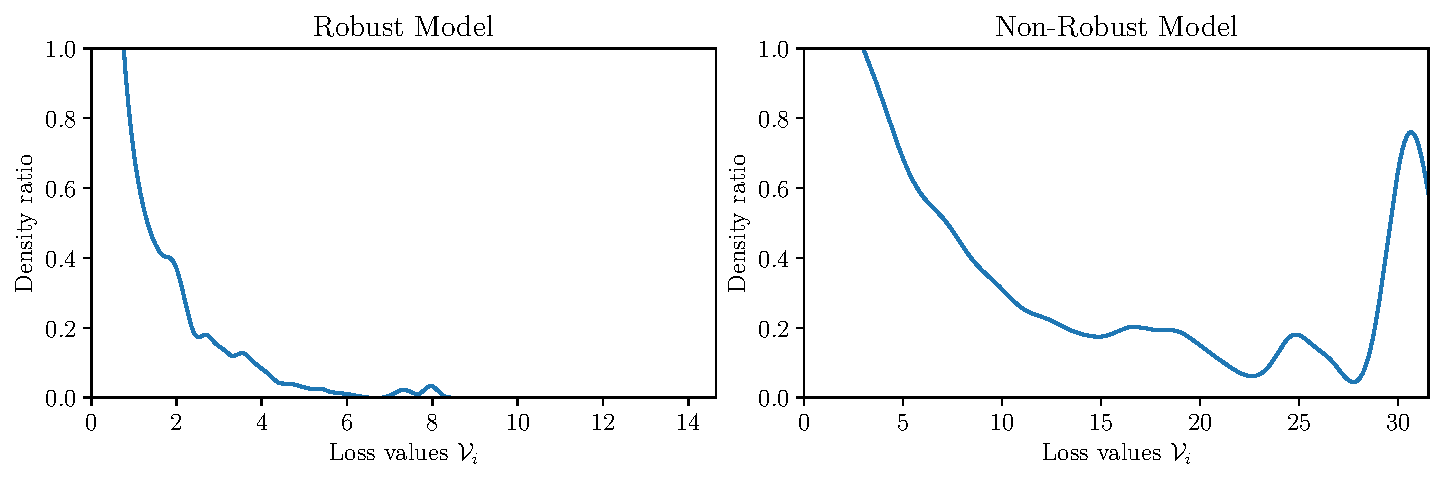
\includegraphics[width=\textwidth]{Figures/density_ratio.pdf}
    \caption{Distribution of the values for robust and non-robust models. We use a gaussian kernel density estimator to estimate the density.}
\label{fig:distrib_values}
\end{figure}

\section*{Societal Impact}
\label{broader_impact}
We introduce the online threat model which aims to capture a new domain for adversarial attack research against streaming data. Such a threat model exposes several new security and privacy risks. For example, using online algorithms, adversaries may now tailor their attack strategy to attacking a small subset of streamed data but still cause significant damage to downstream models e.g. the control system of an autonomous car. On the other hand our research also highlights the need and importance of stateful defence strategies that are capable of mitigating such online attacks. On the theoretical side the development and analysis of \algoname \ has many potential applications outside of adversarial attacks broadly categorized as resource allocation problems. As a concrete example one can consider advertising auctions which provide the main source of monetization for a variety of internet services including search engines, blogs, and social networking sites. Such a scenario is amenable to being modelled as a secretary problem as an advertiser may be able to estimate accurately the bid required to win a particular auction, but may not be privy to the trade off for future auctions.




\end{document}